\documentclass[11pt]{article}
\usepackage{debulletin,times,epsfig,subfigure,wrapfig,algorithmic,color,boxedminipage,graphicx,url}

% this is the template for an issue of the Data Engineering Bulletin

% all packages used by any paper must be listed here
\usepackage{subfig}
\usepackage{listings}
\usepackage{caption}
\usepackage{microtype}
\usepackage{listings}
\usepackage{booktabs}
\usepackage{listings}
\usepackage{xargs}
%\PassOptionsToPackage{hyphens}{url}
%\usepackage{hyperref}
\usepackage{multirow}
\usepackage{tabularx}
\usepackage{makecell}
\usepackage{arydshln}
\usepackage{xspace}
\usepackage{tcolorbox}
\usepackage{xpatch}
\usepackage{amsmath}
\usepackage{tikz}
\usepackage{soul}
\usepackage[lined,boxed,vlined,ruled,linesnumbered]{algorithm2e}
\usepackage[square, numbers]{natbib}




\newcommand{\Hypercallback}{Hyperupcall\xspace{}}
\newcommand{\hypercallback}{hyperupcall\xspace{}}
\newcommand{\hide}[1]{}


\begin{document}


% please enter real date, vol no, issue no
\bulletindate{September 2020}
\bulletinvolume{43}
\bulletinnumber{3}
\bulletinyear{2020}

% these are files that I have- but your part of the issue can be done without
% them
\IEEElogo{cs.pdf}
\insidefrontcover{incvA19.pdf}
%\insidebackcover[ICDE Conference]{./calls/icde-new-a.ps}

\begin{bulletin}

% the above samples assume the issue is generated from a directory structure of the following sort
% major directory name is month and year of issue
% there are sub-directorys for
% letters: directory name is "letters"
% technical articles: a directory per paper, named for an "author"
% news articles: directory name is "news"
% calls: directory name is "calls

%
%  Editor letters section.  Use the lettersection environment.
%  Each letter is contained in a letter environment, where the two required
%  options to \begin{letter} are the author and the address of the author.
%

\begin{lettersection}
% there will be other letters- and a blank page will appear in your document
% but the special issue part will be fine
\begin{letter}{Letter from the Editor-in-Chief}
{Haixun Wang}{WeWork Corporation}
\documentclass[11pt]{article} 

\usepackage{deauthor,times,graphicx}
%\usepackage{url}
\usepackage{hyperref}

\begin{document}
Around the time we published our last issue in March, the nation went
into a lockdown. Life in the last 3 months has been unprecedented in
many ways. As governments around the world scrambled to fight
coronavirus, people in the scientific community, especially those on
the frontline -- doctors, healthcare professionals, medical staff and
researchers -- made heroic efforts and sacrifices to curb the pandemic
and save lives. The data management and data science communities also
sprang to action immediately. Globally, it is the first time that data
driven approaches are being used at such a large scale toward solving
a common problem. Under this backdrop, in this special issue of the
Data Engineering Bulletin edited by Joseph Gonzalez, we feature 8
papers on the topic of {\it digital contact tracing}, a technique that
may prove crucial in the fight against Covid-19.

This issue also features two opinion pieces. Divyakant Agrawal and Amr
El Abbadi's wake-up call on managing data in an untrusted environment
takes us to the fascinating world of cryptocurrencies and
blockchains. It shows what the database community, which was
responsible for creating and perfecting transaction management and
distributed systems, can learn from the blockchain approach when it
comes to handling untrusted behaviours from the underlying
infrastructure. The second opinion piece, written by Jeffrey
D. Ullman, addresses a question on the mind of every data management
person: What is our role in the machine learning and AI revolution?
Have we missed the boat again and become irrelevant? Ullman's
perspective, illustrated by his remake of the well known Conway Venn
Diagram that illustrates the relationship between computer science,
mathematics \& statistics, and domain knowledge is incisive,
thought-provoking, and entertaining at the same time.
\end{document}


\end{letter}
%
\newpage
%
%% your introductory letter goes here
%
\begin{letter}{Letter from the Special Issue Editor}
%{Sihem Amer-Yahia}{CNRS, Univ. Grenoble Alpes}
{Lei Chen}{Hong Kong University of Science and Technology}
\documentclass[11pt]{article} 

\usepackage{deauthor,times,graphicx}
%\usepackage{url}
\usepackage{hyperref}



\begin{document}


Databases have played a very important role in many applications and been widely deployed in many fields. However, traditional database design is still based on empirical methodologies and specifications,  and require heavy human involvement to tune and maintain the databases.   Recently there are many attempts that use AI techniques to optimize database, e.g., learned index, learned cost estimation, learned optimizer, and learning-based database knob tuning. In this issue, we discuss (1) how to adopt AI techniques to optimize databases and (2) how to utilize database techniques to benefit AI and provide in-database capabilities. 

The first paper integrates data preparation into data analysis and adapts data preparation to each workload which can minimize response times.

The second paper discusses how to provide machine learning capabilities inside a database, which is an FPGA-enabled database engine incorporating FPGA-based machine learning operators into a main memory, columnar DBMS. 


The third paper presents two engineering approaches for integrating machine learning agents in a DBMS. The first is to build an external tuning controller that treats the DBMS as a black-box. The second is to integrate the machine learning  agents natively in the DBMS architecture.  

The fourth paper proposes the construction of an engine, a Data Alchemist, which learns how to blend fine-grained data structure design principles to automatically synthesize brand new data structures.

The fifth paper discusses the AutoML problem and proposes MILE, an environment where humans and machines together drive the search for desired ML solutions. 

The last paper proposes an AI-native database. On one hand, it integrates AI techniques into databases to provide self-configuring, self-optimizing, self-monitoring, self-healing, self-diagnosis, self-security and self-assembling capabilities for databases. On the other hand, it can enable databases to provide AI capabilities using declarative languages, in order to lower the barrier of using AI.  



I would like to thank all the authors for their insightful contributions. I hope you enjoy reading the papers. 


\vspace{1em}

\end{document}



\end{letter}

\end{lettersection}

% put the name of your special issue below

\begin{opinionsection}
\begin{opinion}{Resurrecting Middle-Tier Distributed Transactions}
{Philip A. Bernstein}{Microsoft Research, Redmond, WA 98052}
\documentclass[11pt]{article} 
\usepackage{deauthor,times,graphicx,hyperref} 

\begin{document}
\title{Resurrecting Middle-Tier Distributed Transactions}
\author{Philip A. Bernstein\\Microsoft Research\\philbe@microsoft.com}


%\maketitle

\section{Introduction}
Over the years, platforms and application requirements change. As they do, technologies come, go, and return again as the preferred solution to certain system problems. In each of its incarnations, the technology's details change but the principles remain the same. One such technology is distributed transactions on middle-tier servers. Here, we argue that after a 15-year decline, they need to return to the mainstream. 

In the 1980's, Transaction Processing (TP) monitors were a popular category of middleware product that enabled customers to build scalable distributed systems to run transactions. Example products were CICS (IBM), Tuxedo (AT\&T for Unix), ACMS (DEC for VAX/VMS), and Pathway (Tandem for Guardian) \cite{4}. Their main features were multithreaded processes (not supported natively by most operating systems), inter-process communication (usually a crude form of remote procedure call), and a forms manager (for end users to submit transaction requests). The TP monitor ran on middle-tier servers that received transaction requests from front-end processors that communicated with end-user devices, such as terminals and PC's, and with back end database servers. The top-level application code executed on the middle-tier and invoked stored procedures on the database server.  
 
In those days, database management systems (DBMS's) supported ACID transactions, but hardly any of them supported distributed transactions. The TP monitor vendors saw this as a business opportunity and worked on adding a transaction manager feature that implemented the two-phase commit protocol (2PC). Such a feature required DBMS's to expose Start, Prepare, Commit, and Abort as operations that could be invoked by the TP monitor. Unfortunately, most of them didn't support Prepare, and even if they did, they didn't expose it to applications. They were willing to do so, but they didn't want to implement a different protocol for each TP monitor product. Thus, the XA standard was born, which defined TP monitor and DBMS interfaces (including Prepare) and protocols that allowed a TP monitor to run a distributed transaction across DBMS servers \cite{18}. 
 
This middle-tier architecture for distributed transactions was popular for about 20 years, into the late 1990s. Then TP monitors were replaced by Application Servers, which integrated a TP monitor with web servers, so it could receive transaction requests over HTTP, rather than receiving them from devices connected by a local area or terminal network. Examples include Microsoft Transaction Server, later renamed COM+, and Java Enterprise Edition (JEE), implemented by IBM's WebSphere Application Server, Oracle's WebLogic Application Server, and Red Hat's JBoss Application Server \cite{12}. The back end architecture was the same as before. Each transaction started executing on a middle-tier server and invoked stored procedures to read and write the database. 
 
Although this execution model is still widely used, starting in the early 2000's it fell out of favor for new application development, especially for applications targeted for cloud computing. More database vendors offered built-in support for distributed transactions, so there was less need to control the distributed transaction from the middle tier. A larger part of database applications executed on data that was cached in the middle tier. And the NoSQL movement argued that distributed transactions were too slow, that they limited scalability, and that customers rarely needed them anyway \cite{11}. Eventual consistency became all the rage \cite{19}. 
 
The critics of distributed transactions had some good points. But in the end, developers found that mainstream programmers really did need ACID transactions to make their applications reliable in the face of concurrent access to shared data and despite server failures. Thus, some NoSQL (key-value) stores added transaction support (e.g., CosmosDB \cite{2}, DynamoDB \cite{8}). Google, which had initially avoided support for multi-row distributed transactions in Bigtable \cite{5}, later introduced them in Spanner \cite{6}. There are now many cloud storage services and database products that support distributed transactions. 
 
Like product developers, database researchers have also focused on distributed transactions for back-end database systems. Almost universally, they assume that transactions execute as stored procedures and that middle-tier applications invoke those stored procedures but do not execute the transaction logic themselves. 
 
\section{Stateful Middle-Tier Applications}
This focus on stored procedures is well justified by the needs of traditional TP applications. However, stored procedures are not a good way of encapsulating application logic for a growing fraction of stateful applications that run on the middle tier. These include multi-player games, datacenter telemetry, Internet of Things, and social and mobile applications. Objects are a natural model for the entities in these applications, such as games, players, datacenter hardware, sensors, cameras, customers, and smart phones. Such applications have a large number of long-lived stateful objects that are spread over many servers and communicate via message passing. Like most new applications, these applications are usually developed to run on cloud computing platforms.  
 
These applications typically execute on middle-tier servers, rather than as stored procedures in database servers. They do this for many reasons. They need large main memory for the state of long-lived objects. They often have heavy computation needs, such as rendering images or computing over large graphs. They use a lot of computation for message passing between objects so they can scale out. And they need computation to be elastic, independent of storage requirements. These needs are satisfied by compute servers that are cheaper than database servers because they have less storage. Hence, these apps run on compute servers in the middle tier.  

\subsection{Requirements for Mid-Tier Cloud Transactions}
Some middle-tier applications need transactions because they have functions that read and write the state of two or more stateful objects. For example, a game may allow users to buy and sell virtual game objects, such as weapons, shields, and vehicles. A telemetry application may need to process an event exactly once by removing it from a queue and updating telemetry objects based on that event. A social application may need to add a user to a group and modify the user's state to indicate membership in that group. Each of these cases needs an ACID transaction over two or more objects, which may be distributed on different servers. Since these applications are usually developed to run on cloud computing platforms, distributed transaction support must be built into the cloud platform, a capability that is rarely supported today for cloud computing. 
 
Distributed transactions for middle-tier applications on a cloud computing platform have four requirements that differ from those supported by the late-1990's products that run transactions on the middle-tier. First, like all previous transaction mechanisms, they need to offer excellent performance. But unlike previous mechanisms, it's essential that they be able to scale out to a large number of servers, leading to the first requirement: The system must have high throughput and low transaction latency, at least when transactions have low contention, and in addition must scale out to many servers.  

To scale computation independently of storage, these applications typically save their state in cloud storage. The developers' choice of cloud storage service depends on their application's requirements (e.g., records, documents, blobs, SQL), their platform provider's offerings (e.g., AWS, Azure, Google), their employer's storage standards, and their developers' expertise. Thus, we have this second requirement: The transaction mechanism must support applications that use any cloud storage service.  

The transaction mechanism needs persistent storage to track transaction state: started, prepared, committed, or aborted. Like the apps themselves, it needs to use cloud storage for this purpose, which is the third requirement: The transaction mechanism must be able to use any of the cloud storage services used by applications. 

The traditional data structure for storing transaction state is a log. The transaction manager relies on the order of records in the log to understand the order in which transactions executed. Although cloud vendors implement logs to support their database services, they do not expose database-style logging as a service for customers, leading to a fourth requirement: The transaction mechanism cannot rely on a shared log, unless it implements the log itself, in which case the log must run on a wide variety of storage services. 
 
Due to the latency of cloud storage, requirements (2)-(4) create challenges in satisfying requirement (1). 

The above requirements are a first cut, based on today's applications and platforms. It is also worth targeting variations. For example, requirement (1) could include cost/performance, which might require a tradeoff against scalability. And (4) might go away entirely if cloud platforms offer high-performance logging as a service. 

\section{An Implementation in the Orleans Framework}
The rest of this paper sketches a distributed transaction mechanism that satisfies the above requirements \cite{9}. Our group built it for Microsoft's actor-oriented programming framework, called Orleans, which is open source and runs on both Windows and Linux \cite{16}. The distributed transaction project is part of a longer-term effort to enrich Orleans with other database features to evolve it into an actor-oriented database system that supports geo-distribution, stream processing, indexing, and other database features \cite{3}. 
\subsection{Two-Phase Commit and Locking}
For ACID semantics, Orleans transactions use two-phase commit (2PC) and two-phase locking (2PL). Our first challenge was to obtain high throughput and scalability despite the requirement to use cloud storage. In our runs, a write to cloud storage within a datacenter takes ~20 ms and has high variance. With 2PC, a transaction does two synchronous writes to storage. Therefore, if 2PL is used, a transaction holds locks for ~40ms, which limits throughput to 25 transactions/second (TPS). Low-latency SSD-based cloud storage is faster, but still incurs over 10 ms latency, plus higher cost. 
To avoid this problem, we extended early lock release to 2PC \cite{1,7,10,13,14,15}. After a transaction T1 terminates, it releases locks before writing to storage in phase one of 2PC. This allows a later transaction T2 to read/update T1's updated objects. Thus, while T1 is writing to storage, a sequence of later transactions can update an object, terminate, and then unlock the object. To avoid inconsistency, the system delays committing transactions that directly or indirectly read or overwrite T1's writeset until after T1 commits. And if T1 aborts, then those later dependent transactions abort too. Using this mechanism, we have seen transaction throughput up to 20x that of strict 2PL/2PC. 
\subsection{Logging}
Our initial implementation used a centralized transaction manager (TM) per server cluster \cite{9}. It ran on an independent server and was multithreaded. Since message-passing is a potential bottleneck, it batched its messages to transaction servers. It worked well with throughput up to 100K TPS. However, it had three disadvantages: it was an obvious bottleneck for higher transaction rates; a minimum configuration required two servers (i.e., primary and backup TM) in addition to servers that execute the application; and it added configuration complexity since TM servers did not run Orleans and thus had to be deployed separately from application servers.  

These disadvantages led us to redesign the system to avoid a centralized TM. Instead, we embed a TM in each application object. Each TM's log is piggybacked on its object's storage. This TM-per-object design avoids the above disadvantages and improves transaction latency by avoiding roundtrips to a centralized TM. However, it doesn't work for objects that have no updatable storage. For example, an object that performs a money transfer calls two stateful objects, the source and target of the transfer, but it has no state itself. We allow such an object to participate in a transaction by delegating its TM function to a stateful participant in the transaction, that is, one that has updatable storage.  

Orleans transactions write object state to a log to enable undo when a transaction aborts. This is impractical for large objects and is a poor fit for concurrency control that exploits operation commutativity. We therefore developed a prototype that logs operations.  
\section{Summary}
Many new cloud applications run their logic on the middle tier, not as stored procedures. They need distributed transactions. Thus, cloud computing platforms can and should offer scalable distributed transactions.  
\section{Acknowledgments}
I'm grateful to the team that built the initial and final implementations of Orleans transactions: Jason Bragg, Sebastian Burckhardt, Tamer Eldeeb, Reuben Bond, Sergey Bykov, Christopher Meiklejohn, Alejandro Tomsic, and Xiao Zeng. I also thank Bailu Ding and Dave Lomet for suggesting many improvements to this paper. 
 
 
\vspace{-.1cm}
\bibliographystyle{ACM-Reference-Format}
\begin{thebibliography}{10}
\begin{small}
\itemsep=-.5pt
\bibitem{1}
Athanassoulis, Manos ; Johnson, Ryan ; Ailamaki, Anastasia ; Stoica, Radu, Improving OLTP Concurrency through Early Lock Release, EPFL-REPORT-152158, https://infoscience.epfl.ch/record/152158?ln=en, 2009. 

\bibitem{2}
Azure CosmosDB, https://azure.microsoft.com/en-us/services/cosmos-db/ 

\bibitem{3}
Bernstein, P.A., M., T. Kiefer, D. Maier: Indexing in an Actor-Oriented Database. CIDR 2017  

\bibitem{4}
Bernstein, P. A., E. Newcomer: Chapter 10: Transactional Middleware Products and Standards, in Principles of Transaction Processing, Morgan Kaufmann, 2nd ed., 2009. 

\bibitem{5}
Chang, F., J. Dean, S. Ghemawat, W.C. Hsieh, D.A. Wallach, M. Burrows, T. Chandra, A. Fikes, R.E. Gruber: Bigtable: A Distributed Storage System for Structured Data. ACM Trans. Comput. Syst. 26(2): 4:1-4:26 (2008) 


\bibitem{6}
%Corbett, J.C., J. Dean, M. Epstein, A. Fikes, C. Frost, J.J. Furman, S. Ghemawat, A. Gubarev, C. Heiser, P. Hochschild, W.C. Hsieh, S. Kanthak, E. Kogan, H. Li, A. Lloyd, S. Melnik, D. Mwaura, D. Nagle, S. Quinlan, R. Rao, L. Rolig, Y. Saito, M. Szymaniak, C. Taylor, R. Wang, D. Woodford: Spanner: Google's Globally Distributed Database. ACM Trans. Comput. Syst. 31(3): 8:1-8:22 (2013) 
Corbett, J.C. et al: Spanner: Google's Globally Distributed Database. ACM Trans. Comput. Syst. 31(3): 8:1-8:22 (2013) 
\bibitem{7}
DeWitt, D.J., R.H. Katz, F. Olken, L.D. Shapiro, M. Stonebraker, D.A. Wood: Implementation Techniques for Main Memory Database Systems. SIGMOD 1984: 1-8 

\bibitem{8}
DynamoDB, https://aws.amazon.com/dynamodb/ 

\bibitem{9}
Eldeeb, T. and P. Bernstein: Transactions for Distributed Actors in the Cloud. Microsoft Research Tech Report MSR-TR-2016-1001. 

\bibitem{10}
Graefe, G., M. Lillibridge, H. A. Kuno, J. Tucek, A.C. Veitch: Controlled lock violation. SIGMOD 2013: 85-96 

\bibitem{11}
Helland, P., Life beyond Distributed Transactions: an Apostate's Opinion. CIDR 2007: 132-141 

\bibitem{12}
Java EE documentation, http://www.oracle.com/technetwork/?java/javaee/documentation/index.html  

\bibitem{13}
Larson, P-A, et al.: High-Perf. Concurrency Control Mechanisms for Main-Memory Databases. PVLDB 5(4): 298-309 (2011) 
\bibitem{14}

Levandoski, L.J., D.B. Lomet, S. Sengupta, R. Stutsman, R. Wang: High Performance Transactions in Deuteronomy. CIDR 2015 

\bibitem{15}
David B. Lomet: Using Timestamping to Optimize Two Phase Commit. PDIS 1993: 48-55 

\bibitem{16}
Orleans, http://dotnet.github.io/orleans 

\bibitem{18}
The Open Group, Distributed Transaction Processing: The XA Specification, http://pubs.opengroup.org/onlinepubs/009680699/toc.pdf. 

\bibitem{19}
Vogels W., Eventually Consistent. ACM Queue 6(6): 14-19 (2008) \end{small}
\end{thebibliography}

\end{document}

\end{opinion}
\end{opinionsection}

\begin{articlesection}{Human Powered AI Systems}

\begin{article}
	{Computational Division of Labor with Human and AI Workers}
	{Atsuyuki Morishima}
	\pdfminorversion=5
\documentclass[11pt]{article}
\usepackage{deauthor,times,graphicx,caption,microtype}
\usepackage{hyperref}
\usepackage{listings}
\usepackage{booktabs}

\begin{document}

\title{Optimistic Lock Coupling: A Scalable and Efficient General-Purpose Synchronization Method}

\author{Viktor Leis, Michael Haubenschild\raisebox{0.9ex}{$\ast$}, Thomas Neumann\\ Technische Universit{\"a}t M{\"u}nchen \hspace{0.7cm} Tableau Software\raisebox{0.9ex}{$\ast$} \\ {\{leis,neumann\}{@}in.tum.de} \hspace{0.7cm} {mhaubenschild{@}tableau.com\raisebox{0.9ex}{$\ast$}}}

\maketitle

\begin{abstract}
As the number of cores on commodity processors continues to increase, scalability becomes more and more crucial for overall performance.
Scalable and efficient concurrent data structures are particularly important, as these are often the building blocks of parallel algorithms.
Unfortunately, traditional synchronization techniques based on fine-grained locking have been shown to be unscalable on modern multi-core CPUs.
Lock-free data structures, on the other hand, are extremely difficult to design and often incur significant overhead.

In this work, we make the case for Optimistic Lock Coupling as a practical alternative to both traditional locking and the lock-free approach.
We show that Optimistic Lock Coupling is highly scalable and almost as simple to implement as traditional lock coupling.
Another important advantage is that it is easily applicable to most tree-like data structures.
We therefore argue that Optimistic Lock Coupling, rather than a complex and error-prone custom synchronization protocol, should be the default choice for performance-critical data structures.
\end{abstract}

\section{Introduction}

% more and more cores
Today, Intel's commodity server processors have up to 28 cores and its upcoming microarchitecture will have up to 48 cores per socket~\cite{intel}.
Similarly, AMD currently stands at 32 cores and this number is expected to double in the next generation~\cite{amd}.
Since both platforms support simultaneous multithreading (also known as hyperthreading), affordable commodity servers (with up to two sockets) will soon routinely have between 100 and 200 hardware threads.

% data structure scalability is important
With such a high degree of hardware parallelism, efficient data processing crucially depends on how well concurrent data structures scale.
Internally, database systems use a plethora of data structures like table heaps, internal work queues, and, most importantly, index structures.
Any of these can easily become a scalability (and therefore overall performance) bottleneck on many-core CPUs.

% traditional synchronization: fine-grained locks, slow, cache invalidation
Traditionally, database systems synchronize internal data structures using fine-grained reader/writer locks\footnote{In this work, we focus on data structure synchronization rather than high-level transaction semantics and therefore use the term {\em lock} for what would typically be called {\em latch} in the database literature. We thus follow common computer science (rather than database) terminology.}.
Unfortunately, while fine-grained locking makes lock contention unlikely, it still results in bad scalability because lock acquisition and release require writing to shared memory.
Due to the way cache coherency is implemented on modern multi-core CPUs, these writes cause additional cache misses\footnote{The cache coherency protocol ensures that all copies of a cache line on other cores are invalidated before the write can proceed.} and the cache line containing the lock's internal data becomes a point of physical contention.
As a result, any frequently-accessed lock (e.g., the lock of the root node of a B-tree) severely limits scalability.

% lock-free bw-tree: no more latches, but indirections, extremely complex
Lock-free data structures like the Bw-tree~\cite{DBLP:conf/icde/LevandoskiLS13a} (a lock-free B-tree variant) or the Split-Ordered List~\cite{DBLP:journals/jacm/ShalevS06} (a lock-free hash table) do not acquire any locks and therefore generally scale much better than locking-based approaches (in particular for read-mostly workloads).
However, lock-free synchronization has other downsides:
First, it is very difficult and results in extremely complex and error-prone code (when compared to locking).
Second, because the functionality of atomic primitives provided by the hardware (e.g., atomically compare-and-swap 8 bytes) is limited, complex operations require additional indirections within the data structure.
For example, the Bw-tree requires an indirection table and the Split-Ordered List requires ``dummy nodes'', resulting in overhead due to additional cache misses.

% OLC for the win
In this paper we make the case for {\em Optimistic Lock Coupling (OLC)}, a synchronization method that combines some of the best properties of lock-based and lock-free synchronization.
OLC utilizes a special lock type that can be used in two modes:
The first mode is similar to a traditional mutex and excludes other threads by physically acquiring the underlying lock.
In the second mode, reads can proceed optimistically by validating a version counter that is embedded in the lock (similar to optimistic concurrency control).
The first mode is typically used by writers and the second mode by readers.
Besides this special lock type, OLC is based on the observation that optimistic lock validations can be interleaved/coupled---similar to the pair-wise interleaved lock acquisition of traditional lock coupling.
Hence, the name Optimistic Lock Coupling.

OLC has a number of desirable features:
\begin{itemize}
\item By reducing the number of writes to shared memory locations and thereby avoiding cache invalidations, it {\bf scales well} for most workloads.
\item In comparison to unsynchronized code, it requires few additional CPU instructions making it {\bf efficient}.
\item OLC is {\bf widely applicable} to different data structures. It has already been successfully used for synchronizing binary search trees~\cite{DBLP:conf/ppopp/BronsonCCO10}, tries~\cite{artsync}, trie/B-tree hybrids~\cite{DBLP:dblp_conf/eurosys/MaoKM12}, and B-trees~\cite{buzzword}.
\item In comparison to the lock-free paradigm, it is also {\bf easy to use} and requires few modifications to existing, single-threaded data structures.
\end{itemize}
Despite these positive features and its simplicity, OLC is not yet widely known.
The goal of this paper is therefore to popularize this simple idea and to make a case for it.
We argue that OLC deserves to be widely known.
It is a good default synchronization paradigm---more complex, data structure-specific protocols are seldom beneficial.

The rest of the paper is organized as follows.
Section~\ref{sec:related} discusses related work, tracing the history of OLC and its underlying ideas in the literature.
The core of the paper is Section~\ref{sec:olc}, which describes the ideas behind OLC and how it can be used to synchronize complex data structures.
In Section~\ref{sec:evaluation} we experimentally show that OLC has low overhead and scales well when used to synchronize an in-memory B-tree.
We summarize the paper in Section~\ref{sec:conc}.

\newpage
\section{Related Work}\label{sec:related}

Lock coupling has been proposed as a method for allowing concurrent operations on B-trees in 1977~\cite{DBLP:journals/acta/BayerS77}.
This traditional and still widely-used method, described in detail in Graefe's B-tree survey~\cite{DBLP:journals/ftdb/Graefe11}, is also called ``latch coupling'', ``hand-over-hand locking'', and ``crabbing''.
Because at most two locks are held at-a-time during tree traversal, this technique seemingly allows for a high degree of parallelism---in particular if read/write locks are used to enable inner nodes to be locked in shared mode.
However, as we show in Section~\ref{sec:evaluation}, on modern hardware lock acquisition (even in shared mode) results in suboptimal scalability.

An early alternative from 1981 is a B-tree variant called B-link tree~\cite{DBLP:journals/tods/LehmanY81}, which only holds a single lock at a time.
It is based on the observation that between the release of the parent lock and the acquisition of the child lock, the only ``dangerous'' thing that could have happened is the split of a child node (assuming one does not implement merge operations).
Thus, when a split happens, the key being searched might end up on a neighboring node to the right of the current child node.
A B-link tree traversal therefore detects this condition and, if needed, transparently proceeds to the neighboring node.
Releasing the parent lock early is highly beneficial when the child node needs to be fetched from disk.
For in-memory workloads, however, the B-link tree has the same scalability issues as lock coupling (it acquires just as many locks).

The next major advance, Optimistic Latch-Free Index Traversal (OLFIT)~\cite{DBLP:conf/vldb/ChaHKK01}, was proposed in 2001.
OLFIT introduced the idea of a combined lock/update counter, which we call {\em optimistic lock}. % , for lack of a better name,
Based on these per-node optimistic locks and the synchronization protocol of the B-link tree, OLFIT finally achieves good scalability on parallel processors.
The OLFIT protocol is fairly complex, as it requires both the non-trivial B-link protocol and optimistic locks.
Furthermore, like the B-link tree protocol, it does not support merging nodes, and is specific to B-trees (cannot easily be applied to other data structures).

In the following two decades, the growth of main-memory capacity led to much research into other data structures besides the venerable B-tree.
Particularly relevant for our discussion is Bronson et al.'s~\cite{DBLP:conf/ppopp/BronsonCCO10} concurrent binary search tree, which is based on optimistic version validation and has a sophisticated, data structure-specific synchronization protocol.
To the best of our knowledge, this 2010 paper is the first that, as part of its protocol, interleaves version validation across nodes---rather than validating each node separately like OLFIT.
In that paper, this idea is called ``hand-over-hand, optimistic validation'', while we prefer the term Optimistic Lock Coupling to highlight the close resemblance to traditional lock coupling.
Similarly, Mao et al.'s~\cite{DBLP:dblp_conf/eurosys/MaoKM12} Masstree (a concurrent hybrid trie/B-tree) is also based on the same ideas, but again uses them as part of a more complex protocol.

The Adaptive Radix Tree (ART)~\cite{art} is another recent in-memory data structure, which we proposed in 2013.
In contrast to the two data structures just mentioned, it was originally designed with single-threaded performance in mind without supporting concurrency.
To add support for concurrency, we initially started designing a custom protocol called Read-Optimized Write Exclusion (ROWEX)~\cite{artsync}, which turned out to be non-trivial and requires modifications of the underlying data structure\footnote{Note that ROWEX is already easier to apply to existing data structures than the lock-free approach. The difficulty depends on the data structure. Applying ROWEX is hard for B-trees with sorted keys and fairly easy for copy-on-write data structures like the Height Optimized Trie~\cite{hot}---with ART being somewhere in the middle.}.
However, fairly late in the project, we also realized, that OLC {\em alone} (rather than as part of a more complex protocol) is sufficient to synchronize ART.
No other changes to the data structure were necessary.
Both approaches were published and experimentally evaluated in a followup paper~\cite{artsync}, which shows that, despite its simplicity, OLC is efficient, scalable, and generally outperforms ROWEX.

Similar results were recently published regarding B-trees~\cite{buzzword}.
In this experimental study a simple OLC-based synchronization outperformed the Bw-tree~\cite{DBLP:conf/icde/LevandoskiLS13a}, a complex lock-free synchronization approach.
Another recent paper shows that for write-intensive workloads, locking often performs better than lock-free synchronization~\cite{DBLP:conf/cidr/FaleiroA17}.
These experiences indicate that OLC is a general-purpose synchronization paradigm and motivate the current paper.

%foster b-tree\cite{DBLP:journals/tods/GraefeKK12}
%Shasha theory~\cite{DBLP:journals/tods/ShashaG88}

\section{Optimistic Lock Coupling}\label{sec:olc}

% locks suck
The standard technique for inter-thread synchronization is mutual exclusion using fine-grained locks.
In a B-tree, for example, every node usually has its own associated lock, which is acquired before accessing that node.
The problem of locking on modern multi- and many-core processors is that lock acquisition and release require writing to the shared memory location that implements the lock.
This write causes exclusive ownership of the underlying cache line and invalidates copies of it on all other processor cores.
For hierarchical, tree-like data structures, the lock of the root node becomes a point of physical contention---even in read-only workloads and even when read/write locks are used.
Depending on the specific data structure, number of cores, cache coherency protocol implementation, cache topology, whether Non-Uniform Memory Access (NUMA) is used, locking can even result in multi-threaded performance that is worse than single-threaded execution.

% in b-trees this happens very much
The inherent pessimism of locking is particularly unfortunate for B-trees:
Despite the fact that logical modifications of the root node are very infrequent, every B-tree operation must lock the root node during tree traversal\footnote{To a lesser extent this obviously applies to all inner nodes, not just the root.}.
Even the vast majority of update operations (with the exception of splits and merges), only modify a single leaf node.
These observations indicate that a more optimistic approach, which does not require locking inner nodes, would be very beneficial for B-trees.

\subsection{Optimistic Locks}

% optimism to the rescue
As the name indicates, optimistic locks try to solve the scalability issues of traditional locks using an optimistic approach.
Instead of always physically acquiring locks, even for nodes that are unlikely to be modified simultaneously, after-the-fact validation is used to detect conflicts.
This is done by augmenting each lock with a version/update counter that is incremented on every modification.
Using this version counter, readers can optimistically proceed before validating that the version did not change to ensure that the read was safe.
If validation fails, the operation is restarted.

% details on opt locks
Using optimistic locks, a read-only node access (i.e., the majority of all operations in a B-tree) does not acquire the lock and does not increment the version counter.
Instead, it performs the following steps:
\begin{enumerate}
\item read lock version (restart if lock is not free)
\item access node
\item read the version again and validate that it has not changed in the meantime
\end{enumerate}
If the last step (the validation) fails, the operation has to be restarted.
Write operations, on the other hand, are more similar to traditional locking:
\begin{enumerate}
\item acquire lock (wait if necessary)
\item access/write to node
\item increment version and unlock node
\end{enumerate}
Writes can therefore protect a node from other writes.

% similar to locks
As we observed in an earlier paper~\cite{artsync}, because of similar semantics, optimistic locks can be hidden behind an API very similar to traditional read/write locks.
Both approaches have an exclusive lock mode, and acquiring a traditional lock in shared mode is analogous to optimistic version validation.
Furthermore, like with some implementations of traditional read/write locks, optimistic locks allow upgrading a shared lock to an exclusive lock.
Lock upgrades are, for example, used to avoid most B-tree update operations from having to lock inner nodes.
In our experience, the close resemblance of optimistic and traditional locks simplifies the reasoning about optimistic locks;
one can apply similar thinking as in traditional lock-based protocols.

\subsection{Lock Coupling with Optimistic Locks}

\begin{figure}
  \centering
  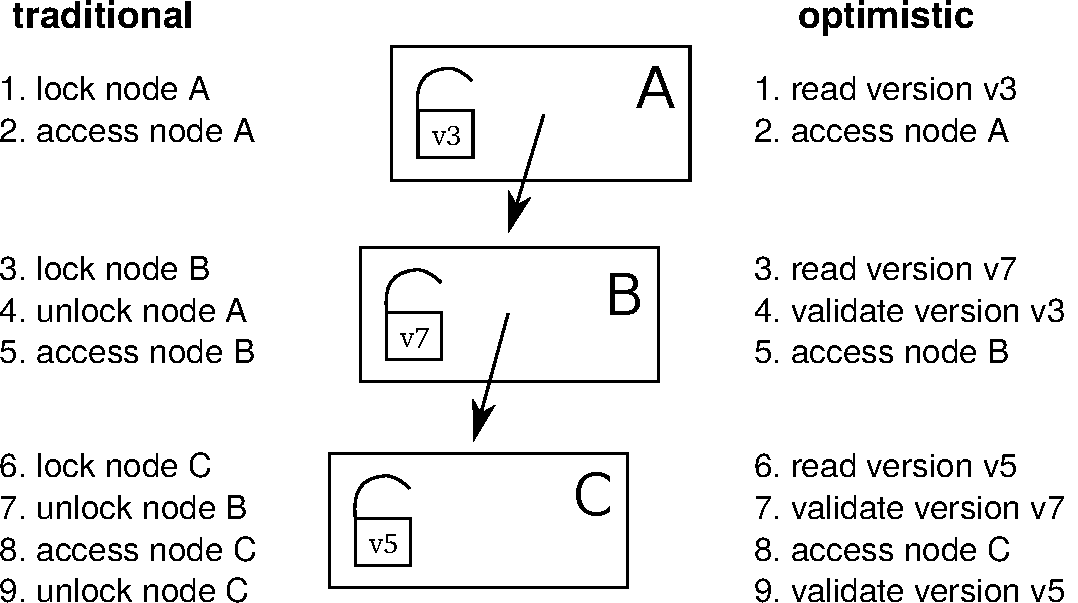
\includegraphics[width=0.65\linewidth]{olcall.pdf}
  \vspace{0.2cm}
  \caption{Comparison of a lookup operation in a 3-level tree using traditional lock coupling (left-hand side) vs.~optimistic lock coupling (right-hand side).}
  \label{fig:olc}
\end{figure}

The traditional and most common lock-based synchronization protocol for B-trees is lock coupling, which interleaves lock acquisitions while holding at most two locks at a time.
If, as we observed earlier, optimistic locks have similar semantics as traditional locks, it is natural to ask whether lock coupling can be combined with optimistic locks.
And indeed the answer is yes: One can almost mechanically translate traditional lock coupling code to optimistic lock coupling code.
This is illustrated in Figure~\ref{fig:olc}, which compares the traversal in a tree of height 3 using traditional and optimistic locks.
As the figure shows, the main difference is that locking is translated to reading the version and that unlocking becomes validation of the previously read version.
This simple change provides efficient lock-free tree traversal without the need to design a complex synchronization protocol.

It is important to emphasize the conceptual simplicity of OLC in comparison to data structures that use custom protocols like the Bw-tree~\cite{DBLP:conf/icde/LevandoskiLS13a}.
To implement lock-free access, the Bw-tree requires an indirection table, delta nodes, complex splitting and merging logic, retry logic, etc.
OLC, on the other hand, can directly be applied to B-trees mostly by adding the appropriate optimistic locking code and without modifying the node layout itself.
Therefore, OpenBw-Tree, an open source implementation of the Bw-tree, requires an order of magnitude more code than a B-tree based on OLC\footnote{Both implementations are available on GitHub: \url{https://github.com/wangziqi2016/index-microbench}}.
Given how difficult it is to develop, validate, and debug lock-free code, simplicity is obviously a major advantage.

\subsection{Correctness Aspects}

\begin{figure}
  % \centering
  %[basicstyle=\normalsize\ttfamily,showstringspaces=false,columns=fullflexible,breaklines=false,breakatwhitespace=true,numbers=none,numberstyle=\small,style=C,keepspaces=true]
\begin{lstlisting}[basicstyle=\ttfamily,language=C++,numbers=left,numberstyle=\small]
std::atomic<BTreeNode*> root;

// search for key in B+tree, returns payload in resultOut
bool lookup(Key key, Value& resultOut) {
   BTreeNode* node = root.load();
   uint64_t nodeVersion = node->readLockOrRestart();
   if (node != root.load()) // make sure the root is still the root
      restart();

   BTreeInner<Key>* parent = nullptr;
   uint64_t parentVersion = 0;

   while (node->isInner()) {
      auto inner = (BTreeInner*)node;

      // unlock parent and make current node the parent
      if (parent)
         parent->readUnlockOrRestart(parentVersion);
      parent = inner;
      parentVersion = nodeVersion;

      // search for next node
      node = inner->findChild(key);
      // validate 'inner' to ensure that 'node' pointer is valid
      inner->checkOrRestart(nodeVersion);
      // now it safe to dereference 'node' pointer (read its version)
      nodeVersion = node->readLockOrRestart();
   }

   // search in leaf and retrieve payload
   auto leaf = (BTreeLeaf*)node;
   bool success = leaf->findValue(key, resultOut);

   // unlock everything
   if (parent)
      parent->readUnlockOrRestart(parentVersion);
   node->readUnlockOrRestart(nodeVersion);

   return success;
}
\end{lstlisting}
  \vspace{0.2cm}
  \caption{B-tree lookup code using OLC. For simplicity, the restart logic is not shown.}
  \label{fig:lookup}
\end{figure}

So far, we have introduced the high-level ideas behind OLC and have stressed its similarity to traditional lock coupling.
Let us now discuss some cases where the close similarity between lock coupling and OLC breaks down.
To make this more concrete, we show the B-tree lookup code in Figure~\ref{fig:lookup}.
In the code, \texttt{readLockOrRestart} reads the lock version and \texttt{readUnlockOrRestart} validates that the read was correct.

One issue with OLC is that any pointer speculatively read from a node may point to invalid memory (if that node is modified concurrently).
Dereferencing such a pointer (e.g., to read its optimistic lock), may cause a segmentation fault or undefined behavior.
In the code shown in Figure~\ref{fig:lookup}, this problem is prevented by the extra check in line 25, which ensures that the read from the node containing the pointer was correct.
Without this additional validation, the code would in line 27 dereference the pointer speculatively read in line 23.
Note that the implementation of \texttt{checkOrRestart} is actually identical to \texttt{readUnlockOrRestart}.
We chose to give it a different name to highlight the fact that this extra check would not be necessary with read/write locks.

Another potential issue with optimistic locks is code that does not terminate.
Code that speculatively accesses a node, like an intra-node binary search, should be written in a way such that it always terminates---even in the presence of concurrent writes.
Otherwise, the validation code that detects the concurrent write will never run.
The binary search of a B-tree, for example, needs to be written in such a way that each comparison makes progress.
For some data structures that do not require loops in the traversal code (like ART) termination is trivially true.

\subsection{Implementation Details}

% implementation, efficiency
To implement an optimistic lock, one can combine the lock and the version counter into a single 64-bit\footnote{Even after subtracting one bit for the lock status, a back-of-the-envelope calculation can show that 63 bits are large enough to never overflow in practice.} word~\cite{artsync}.
A typical read operation will therefore merely consist of reading this version counter atomically.
In C++11 this can be implemented using the \texttt{std::atomic} type.

On x86, atomic reads are cheap because of x86's strong memory order guarantees.
No memory fences are required for sequentially-consistent loads, which are translated (by both GCC and clang) into standard \texttt{MOV} instructions.
Hence, the only effect of \texttt{std::atomic} for loads is preventing instruction re-ordering.
This makes version access and validation cheap.
Acquiring and releasing an optimistic lock in exclusive mode has comparable cost to a traditional lock:
A fairly expensive sequentially-consistent store is needed for acquiring a lock, while a standard \texttt{MOV} suffices for releasing it.
A simple sinlock-based implementation of optimistic locks can be found in the appendix of an earlier paper~\cite{artsync}.

OLC code must be able to handle restarts since validation or lock upgrade can fail due to concurrent writers.
Restarts can easily be implemented by wrapping the data structure operation in a loop (for simplicity not shown in Figure~\ref{fig:lookup}).
Such a loop also enables limiting the number of optimistic retry operations and falling back to pessimistic locking in cases of very heavy contention.
The ability to fall back to traditional locking is a major advantage of OLC in terms of robustness over lock-free approaches, which do not have this option.

In addition to the optimistic shared mode and the exclusive mode, optimistic locks also support a ``shared pessimistic'' mode, which physically acquires the lock in shared mode (allowing multiple concurrent readers but no writers).
This mode is useful for table (or range) scans that touch many tuples on a leaf page (which would otherwise easily abort).
Finally, let us mention that large range scans and table scans, should be broken up into several per-node traversals as is done in the LeanStore~\cite{leanstore} system.

Like all lock-free data structures, but unlike traditional locking and Hardware Transactional Memory~\cite{DBLP:conf/hpca/KarnagelDRLLSL14,DBLP:journals/pvldb/MakreshanskiLS15,htmtkde}, OLC requires care when deleting (and reusing) nodes.
The reason is that a deleting thread can never be sure that a node can be reclaimed because other threads might still be optimistically reading from that node.
Therefore, standard solutions like epoch-based reclamation~\cite{DBLP:conf/sosp/TuZKLM13}, hazard pointers~\cite{DBLP:journals/tpds/Michael04}, or optimized hazard pointers~\cite{DBLP:conf/spaa/BalmauGHZ16} need to be used.
These memory reclamation techniques are, however, largely orthogonal to the synchronization protocol itself.

%-lock-free is not a strong guarantee

\newpage
\section{Evaluation}\label{sec:evaluation}

Let us now experimentally evaluate the overhead and scalability of OLC.
For the experiments, we use an in-memory B+tree implemented in C++11 using templates, which is configured to use nodes of 4096 bytes, random 8 byte keys, and 8 byte payloads.
Based on this B-tree, we compare the following synchronization approaches:
\begin{itemize}
\item an OLC implementation\footnote{An almost identical OLC implementation is available on github: \url{https://github.com/wangziqi2016/index-microbench/tree/master/BTreeOLC}}
\item a variant based on traditional lock coupling and read/write locks
\item the unsynchronized B-tree, which obviously is only correct for read-only workloads but allows measuring the overhead of synchronization
\end{itemize}
Note that earlier work has compared the OLC implementation with a Bw-tree implementation~\cite{buzzword} and other state-of-the-art in-memory index structures.

We use a Haswell EP system with an Intel Xeon E5-2687W v3 CPU, which has 10 cores (20 ``Hyper-Threads'') and 25~MB of L3 cache.
The system is running Ubuntu 18.10 and we use GCC 8.2.0 to compile our code.
The CPU counters are obtained using the Linux perf API\footnote{We use the following convenience wrapper: \url{https://github.com/viktorleis/perfevent}}.

\begin{table}
  \caption{Performance and CPU counters for lookup and insert operations in a B-tree with 100M keys. We perform 100M operations and normalize the CPU counters by that number.}
  \label{tab:overhead}
  \centering
  \begin{tabular}{lrrrrrrr}\toprule
                    &         &        &        & instruc-  & L1     & L3     & branch \\
                    & threads & M op/s & cycles & tions & misses & misses & misses \\\midrule
lookup (no sync.)   & 1       & 1.72   & 2028   & 283     & 39.1   & 14.9   & 16.1   \\
lookup (OLC)        & 1       & 1.65   & 2107   & 370     & 43.9   & 15.1   & 16.7   \\
lookup (lock coup.) & 1       & 1.72   & 2078   & 365     & 42.3   & 16.9   & 15.7   \\\midrule
insert (no sync.)   & 1       & 1.51   & 2286   & 530     & 59.8   & 31.1   & 17.3   \\
insert (OLC)        & 1       & 1.50   & 2303   & 629     & 61.2   & 31.1   & 16.5   \\
insert (lock coup.) & 1       & 1.41   & 2473   & 644     & 61.0   & 31.0   & 17.2   \\\midrule
lookup (no sync.)   & 10      & 15.48  & 2058   & 283     & 38.6   & 15.5   & 16.0   \\
lookup (OLC)        & 10      & 14.60  & 2187   & 370     & 43.8   & 15.8   & 16.8   \\
lookup (lock coup.) & 10      & 5.71   & 5591   & 379     & 54.2   & 17.0   & 14.8   \\\midrule
insert (no sync.)   & 10      & -      & -      & -       & -      & -      & -      \\
insert (OLC)        & 10      & 10.46  & 2940   & 656     & 62.0   & 32.5   & 16.8   \\
insert (lock coup.) & 10      & 7.55   & 4161   & 667     & 75.0   & 28.6   & 16.2   \\
    \bottomrule
\end{tabular}
\end{table}

Table~\ref{tab:overhead} compares the performance and CPU counters for lookup and insert operations in a B-tree with 100M keys.
With {\em single-threaded} execution, we observe that all three approaches have very similar performance.
Adding traditional or optimistic locks to unsynchronized B-tree code results in up to 30\% of additional instructions without affecting single-threaded performance much.

\begin{figure}
  \centering
  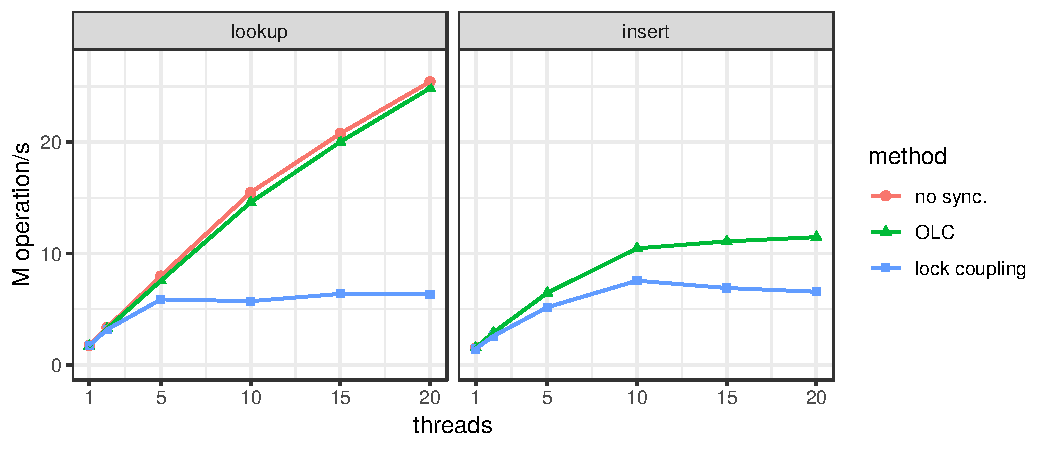
\includegraphics[width=\linewidth]{scale.pdf}
  \vspace{0.2cm}
  \caption{Scalability on 10-core system for B-tree operations (100M values).}
  \label{fig:scale}
\end{figure}

As Figure~\ref{fig:scale} shows, the results change dramatically once we use multiple threads.
For lookup, the scalability of OLC is near-linear up to 20 threads, even though the system has only 10 ``real cores''.
The OLC scalability for insert is also respectable (though not quite as linear because multi-threaded insertion approaches the memory bandwidth of our processor).
The figure also shows that the results of traditional lock coupling with read/write locks are significantly worse than OLC.
With 20 threads, lookup with OLC is 3.9$\times$ faster than traditional lock coupling.

\section{Summary}\label{sec:conc}

Optimistic Lock Coupling (OLC) is an effective synchronization method that combines the simplicity of traditional lock coupling with the superior scalability of lock-free approaches.
OLC is widely applicable and has already been successfully used to synchronize several data structures, including B-trees, binary search trees, and different trie variants.
These features make it highly attractive for modern database systems as well as performance-critical systems software in general.

\begin{thebibliography}{10}

\bibitem{DBLP:conf/spaa/BalmauGHZ16}
O.~Balmau, R.~Guerraoui, M.~Herlihy, and I.~Zablotchi.
\newblock Fast and robust memory reclamation for concurrent data structures.
\newblock In {\em SPAA}, 2016.

\bibitem{DBLP:journals/acta/BayerS77}
R.~Bayer and M.~Schkolnick.
\newblock Concurrency of operations on {B}-trees.
\newblock {\em Acta Informatica}, 9, 1977.

\bibitem{hot}
R.~Binna, E.~Zangerle, M.~Pichl, G.~Specht, and V.~Leis.
\newblock {HOT}: A height optimized trie index for main-memory database
  systems.
\newblock In {\em SIGMOD}, 2018.

\bibitem{DBLP:conf/ppopp/BronsonCCO10}
N.~G. Bronson, J.~Casper, H.~Chafi, and K.~Olukotun.
\newblock A practical concurrent binary search tree.
\newblock In {\em PPOPP}, 2010.

\bibitem{DBLP:conf/vldb/ChaHKK01}
S.~K. Cha, S.~Hwang, K.~Kim, and K.~Kwon.
\newblock Cache-conscious concurrency control of main-memory indexes on
  shared-memory multiprocessor systems.
\newblock In {\em VLDB}, 2001.

\bibitem{intel}
I.~Cutress.
\newblock {Intel} goes for 48-cores: {Cascade-AP} with multi-chip package
  coming soon.
\newblock
  \url{https://www.anandtech.com/show/13535/intel-goes-for-48cores-cascade-ap},
  2018 (accessed January, 2019).

\bibitem{DBLP:conf/cidr/FaleiroA17}
J.~M. Faleiro and D.~J. Abadi.
\newblock Latch-free synchronization in database systems: Silver bullet or
  fool's gold?
\newblock In {\em CIDR}, 2017.

\bibitem{DBLP:journals/ftdb/Graefe11}
G.~Graefe.
\newblock Modern {B}-tree techniques.
\newblock {\em Foundations and Trends in Databases}, 3(4), 2011.

\bibitem{DBLP:conf/hpca/KarnagelDRLLSL14}
T.~Karnagel, R.~Dementiev, R.~Rajwar, K.~Lai, T.~Legler, B.~Schlegel, and
  W.~Lehner.
\newblock Improving in-memory database index performance with
  {Intel}\({}^{\mbox{{\textregistered}}}\) transactional synchronization
  extensions.
\newblock In {\em HPCA}, 2014.

\bibitem{DBLP:journals/tods/LehmanY81}
P.~L. Lehman and S.~B. Yao.
\newblock Efficient locking for concurrent operations on {B}-trees.
\newblock {\em {ACM} Trans. Database Syst.}, 6(4), 1981.

\bibitem{leanstore}
V.~Leis, M.~Haubenschild, A.~Kemper, and T.~Neumann.
\newblock Leanstore: In-memory data management beyond main memory.
\newblock In {\em ICDE}, 2018.

\bibitem{art}
V.~Leis, A.~Kemper, and T.~Neumann.
\newblock The adaptive radix tree: {ARTful} indexing for main-memory databases.
\newblock In {\em ICDE}, 2013.

\bibitem{htmtkde}
V.~Leis, A.~Kemper, and T.~Neumann.
\newblock Scaling {HTM}-supported database transactions to many cores.
\newblock {\em {IEEE} Trans. Knowl. Data Eng.}, 28(2), 2016.

\bibitem{artsync}
V.~Leis, F.~Scheibner, A.~Kemper, and T.~Neumann.
\newblock The {ART} of practical synchronization.
\newblock In {\em DaMoN}, 2016.

\bibitem{DBLP:conf/icde/LevandoskiLS13a}
J.~J. Levandoski, D.~B. Lomet, and S.~Sengupta.
\newblock The {Bw}-tree: A {B}-tree for new hardware platforms.
\newblock In {\em ICDE}, 2013.

\bibitem{DBLP:journals/pvldb/MakreshanskiLS15}
D.~Makreshanski, J.~J. Levandoski, and R.~Stutsman.
\newblock To lock, swap, or elide: On the interplay of hardware transactional
  memory and lock-free indexing.
\newblock {\em {PVLDB}}, 8(11), 2015.

\bibitem{DBLP:dblp_conf/eurosys/MaoKM12}
Y.~Mao, E.~Kohler, and R.~T. Morris.
\newblock Cache craftiness for fast multicore key-value storage.
\newblock In {\em EuroSys}, 2012.

\bibitem{DBLP:journals/tpds/Michael04}
M.~M. Michael.
\newblock Hazard pointers: Safe memory reclamation for lock-free objects.
\newblock {\em {IEEE} Trans. Parallel Distrib. Syst.}, 15(6), 2004.

\bibitem{DBLP:journals/jacm/ShalevS06}
O.~Shalev and N.~Shavit.
\newblock Split-ordered lists: Lock-free extensible hash tables.
\newblock {\em J. {ACM}}, 53(3), 2006.

\bibitem{amd}
A.~Shilov.
\newblock {AMD} previews {EPYC} ‘{Rome}’ processor: Up to 64 {Zen} 2 cores.
\newblock
  \url{https://www.anandtech.com/show/13561/amd-previews-epyc-rome-processor-up-to-64-zen-2-cores},
  2018 (accessed January, 2019).

\bibitem{DBLP:conf/sosp/TuZKLM13}
S.~Tu, W.~Zheng, E.~Kohler, B.~Liskov, and S.~Madden.
\newblock Speedy transactions in multicore in-memory databases.
\newblock In {\em SOSP}, 2013.

\bibitem{buzzword}
Z.~Wang, A.~Pavlo, H.~Lim, V.~Leis, H.~Zhang, M.~Kaminsky, and D.~Andersen.
\newblock Building a {Bw}-tree takes more than just buzz words.
\newblock In {\em SIGMOD}, 2018.

\end{thebibliography}


%\bibliographystyle{abbrv}
%\bibliography{main}

\end{document}

\end{article}

\begin{article}
	{Federated Learning in the Lens of Crowdsourcing}
	{Yongxin Tong,Yansheng Wang,Dingyuan Shi
	}
	\pdfminorversion=5
\documentclass[11pt]{article}
\usepackage{deauthor,times,graphicx,caption,microtype}
\usepackage{hyperref}
\usepackage{listings}
\usepackage{booktabs}

\begin{document}

\title{Optimistic Lock Coupling: A Scalable and Efficient General-Purpose Synchronization Method}

\author{Viktor Leis, Michael Haubenschild\raisebox{0.9ex}{$\ast$}, Thomas Neumann\\ Technische Universit{\"a}t M{\"u}nchen \hspace{0.7cm} Tableau Software\raisebox{0.9ex}{$\ast$} \\ {\{leis,neumann\}{@}in.tum.de} \hspace{0.7cm} {mhaubenschild{@}tableau.com\raisebox{0.9ex}{$\ast$}}}

\maketitle

\begin{abstract}
As the number of cores on commodity processors continues to increase, scalability becomes more and more crucial for overall performance.
Scalable and efficient concurrent data structures are particularly important, as these are often the building blocks of parallel algorithms.
Unfortunately, traditional synchronization techniques based on fine-grained locking have been shown to be unscalable on modern multi-core CPUs.
Lock-free data structures, on the other hand, are extremely difficult to design and often incur significant overhead.

In this work, we make the case for Optimistic Lock Coupling as a practical alternative to both traditional locking and the lock-free approach.
We show that Optimistic Lock Coupling is highly scalable and almost as simple to implement as traditional lock coupling.
Another important advantage is that it is easily applicable to most tree-like data structures.
We therefore argue that Optimistic Lock Coupling, rather than a complex and error-prone custom synchronization protocol, should be the default choice for performance-critical data structures.
\end{abstract}

\section{Introduction}

% more and more cores
Today, Intel's commodity server processors have up to 28 cores and its upcoming microarchitecture will have up to 48 cores per socket~\cite{intel}.
Similarly, AMD currently stands at 32 cores and this number is expected to double in the next generation~\cite{amd}.
Since both platforms support simultaneous multithreading (also known as hyperthreading), affordable commodity servers (with up to two sockets) will soon routinely have between 100 and 200 hardware threads.

% data structure scalability is important
With such a high degree of hardware parallelism, efficient data processing crucially depends on how well concurrent data structures scale.
Internally, database systems use a plethora of data structures like table heaps, internal work queues, and, most importantly, index structures.
Any of these can easily become a scalability (and therefore overall performance) bottleneck on many-core CPUs.

% traditional synchronization: fine-grained locks, slow, cache invalidation
Traditionally, database systems synchronize internal data structures using fine-grained reader/writer locks\footnote{In this work, we focus on data structure synchronization rather than high-level transaction semantics and therefore use the term {\em lock} for what would typically be called {\em latch} in the database literature. We thus follow common computer science (rather than database) terminology.}.
Unfortunately, while fine-grained locking makes lock contention unlikely, it still results in bad scalability because lock acquisition and release require writing to shared memory.
Due to the way cache coherency is implemented on modern multi-core CPUs, these writes cause additional cache misses\footnote{The cache coherency protocol ensures that all copies of a cache line on other cores are invalidated before the write can proceed.} and the cache line containing the lock's internal data becomes a point of physical contention.
As a result, any frequently-accessed lock (e.g., the lock of the root node of a B-tree) severely limits scalability.

% lock-free bw-tree: no more latches, but indirections, extremely complex
Lock-free data structures like the Bw-tree~\cite{DBLP:conf/icde/LevandoskiLS13a} (a lock-free B-tree variant) or the Split-Ordered List~\cite{DBLP:journals/jacm/ShalevS06} (a lock-free hash table) do not acquire any locks and therefore generally scale much better than locking-based approaches (in particular for read-mostly workloads).
However, lock-free synchronization has other downsides:
First, it is very difficult and results in extremely complex and error-prone code (when compared to locking).
Second, because the functionality of atomic primitives provided by the hardware (e.g., atomically compare-and-swap 8 bytes) is limited, complex operations require additional indirections within the data structure.
For example, the Bw-tree requires an indirection table and the Split-Ordered List requires ``dummy nodes'', resulting in overhead due to additional cache misses.

% OLC for the win
In this paper we make the case for {\em Optimistic Lock Coupling (OLC)}, a synchronization method that combines some of the best properties of lock-based and lock-free synchronization.
OLC utilizes a special lock type that can be used in two modes:
The first mode is similar to a traditional mutex and excludes other threads by physically acquiring the underlying lock.
In the second mode, reads can proceed optimistically by validating a version counter that is embedded in the lock (similar to optimistic concurrency control).
The first mode is typically used by writers and the second mode by readers.
Besides this special lock type, OLC is based on the observation that optimistic lock validations can be interleaved/coupled---similar to the pair-wise interleaved lock acquisition of traditional lock coupling.
Hence, the name Optimistic Lock Coupling.

OLC has a number of desirable features:
\begin{itemize}
\item By reducing the number of writes to shared memory locations and thereby avoiding cache invalidations, it {\bf scales well} for most workloads.
\item In comparison to unsynchronized code, it requires few additional CPU instructions making it {\bf efficient}.
\item OLC is {\bf widely applicable} to different data structures. It has already been successfully used for synchronizing binary search trees~\cite{DBLP:conf/ppopp/BronsonCCO10}, tries~\cite{artsync}, trie/B-tree hybrids~\cite{DBLP:dblp_conf/eurosys/MaoKM12}, and B-trees~\cite{buzzword}.
\item In comparison to the lock-free paradigm, it is also {\bf easy to use} and requires few modifications to existing, single-threaded data structures.
\end{itemize}
Despite these positive features and its simplicity, OLC is not yet widely known.
The goal of this paper is therefore to popularize this simple idea and to make a case for it.
We argue that OLC deserves to be widely known.
It is a good default synchronization paradigm---more complex, data structure-specific protocols are seldom beneficial.

The rest of the paper is organized as follows.
Section~\ref{sec:related} discusses related work, tracing the history of OLC and its underlying ideas in the literature.
The core of the paper is Section~\ref{sec:olc}, which describes the ideas behind OLC and how it can be used to synchronize complex data structures.
In Section~\ref{sec:evaluation} we experimentally show that OLC has low overhead and scales well when used to synchronize an in-memory B-tree.
We summarize the paper in Section~\ref{sec:conc}.

\newpage
\section{Related Work}\label{sec:related}

Lock coupling has been proposed as a method for allowing concurrent operations on B-trees in 1977~\cite{DBLP:journals/acta/BayerS77}.
This traditional and still widely-used method, described in detail in Graefe's B-tree survey~\cite{DBLP:journals/ftdb/Graefe11}, is also called ``latch coupling'', ``hand-over-hand locking'', and ``crabbing''.
Because at most two locks are held at-a-time during tree traversal, this technique seemingly allows for a high degree of parallelism---in particular if read/write locks are used to enable inner nodes to be locked in shared mode.
However, as we show in Section~\ref{sec:evaluation}, on modern hardware lock acquisition (even in shared mode) results in suboptimal scalability.

An early alternative from 1981 is a B-tree variant called B-link tree~\cite{DBLP:journals/tods/LehmanY81}, which only holds a single lock at a time.
It is based on the observation that between the release of the parent lock and the acquisition of the child lock, the only ``dangerous'' thing that could have happened is the split of a child node (assuming one does not implement merge operations).
Thus, when a split happens, the key being searched might end up on a neighboring node to the right of the current child node.
A B-link tree traversal therefore detects this condition and, if needed, transparently proceeds to the neighboring node.
Releasing the parent lock early is highly beneficial when the child node needs to be fetched from disk.
For in-memory workloads, however, the B-link tree has the same scalability issues as lock coupling (it acquires just as many locks).

The next major advance, Optimistic Latch-Free Index Traversal (OLFIT)~\cite{DBLP:conf/vldb/ChaHKK01}, was proposed in 2001.
OLFIT introduced the idea of a combined lock/update counter, which we call {\em optimistic lock}. % , for lack of a better name,
Based on these per-node optimistic locks and the synchronization protocol of the B-link tree, OLFIT finally achieves good scalability on parallel processors.
The OLFIT protocol is fairly complex, as it requires both the non-trivial B-link protocol and optimistic locks.
Furthermore, like the B-link tree protocol, it does not support merging nodes, and is specific to B-trees (cannot easily be applied to other data structures).

In the following two decades, the growth of main-memory capacity led to much research into other data structures besides the venerable B-tree.
Particularly relevant for our discussion is Bronson et al.'s~\cite{DBLP:conf/ppopp/BronsonCCO10} concurrent binary search tree, which is based on optimistic version validation and has a sophisticated, data structure-specific synchronization protocol.
To the best of our knowledge, this 2010 paper is the first that, as part of its protocol, interleaves version validation across nodes---rather than validating each node separately like OLFIT.
In that paper, this idea is called ``hand-over-hand, optimistic validation'', while we prefer the term Optimistic Lock Coupling to highlight the close resemblance to traditional lock coupling.
Similarly, Mao et al.'s~\cite{DBLP:dblp_conf/eurosys/MaoKM12} Masstree (a concurrent hybrid trie/B-tree) is also based on the same ideas, but again uses them as part of a more complex protocol.

The Adaptive Radix Tree (ART)~\cite{art} is another recent in-memory data structure, which we proposed in 2013.
In contrast to the two data structures just mentioned, it was originally designed with single-threaded performance in mind without supporting concurrency.
To add support for concurrency, we initially started designing a custom protocol called Read-Optimized Write Exclusion (ROWEX)~\cite{artsync}, which turned out to be non-trivial and requires modifications of the underlying data structure\footnote{Note that ROWEX is already easier to apply to existing data structures than the lock-free approach. The difficulty depends on the data structure. Applying ROWEX is hard for B-trees with sorted keys and fairly easy for copy-on-write data structures like the Height Optimized Trie~\cite{hot}---with ART being somewhere in the middle.}.
However, fairly late in the project, we also realized, that OLC {\em alone} (rather than as part of a more complex protocol) is sufficient to synchronize ART.
No other changes to the data structure were necessary.
Both approaches were published and experimentally evaluated in a followup paper~\cite{artsync}, which shows that, despite its simplicity, OLC is efficient, scalable, and generally outperforms ROWEX.

Similar results were recently published regarding B-trees~\cite{buzzword}.
In this experimental study a simple OLC-based synchronization outperformed the Bw-tree~\cite{DBLP:conf/icde/LevandoskiLS13a}, a complex lock-free synchronization approach.
Another recent paper shows that for write-intensive workloads, locking often performs better than lock-free synchronization~\cite{DBLP:conf/cidr/FaleiroA17}.
These experiences indicate that OLC is a general-purpose synchronization paradigm and motivate the current paper.

%foster b-tree\cite{DBLP:journals/tods/GraefeKK12}
%Shasha theory~\cite{DBLP:journals/tods/ShashaG88}

\section{Optimistic Lock Coupling}\label{sec:olc}

% locks suck
The standard technique for inter-thread synchronization is mutual exclusion using fine-grained locks.
In a B-tree, for example, every node usually has its own associated lock, which is acquired before accessing that node.
The problem of locking on modern multi- and many-core processors is that lock acquisition and release require writing to the shared memory location that implements the lock.
This write causes exclusive ownership of the underlying cache line and invalidates copies of it on all other processor cores.
For hierarchical, tree-like data structures, the lock of the root node becomes a point of physical contention---even in read-only workloads and even when read/write locks are used.
Depending on the specific data structure, number of cores, cache coherency protocol implementation, cache topology, whether Non-Uniform Memory Access (NUMA) is used, locking can even result in multi-threaded performance that is worse than single-threaded execution.

% in b-trees this happens very much
The inherent pessimism of locking is particularly unfortunate for B-trees:
Despite the fact that logical modifications of the root node are very infrequent, every B-tree operation must lock the root node during tree traversal\footnote{To a lesser extent this obviously applies to all inner nodes, not just the root.}.
Even the vast majority of update operations (with the exception of splits and merges), only modify a single leaf node.
These observations indicate that a more optimistic approach, which does not require locking inner nodes, would be very beneficial for B-trees.

\subsection{Optimistic Locks}

% optimism to the rescue
As the name indicates, optimistic locks try to solve the scalability issues of traditional locks using an optimistic approach.
Instead of always physically acquiring locks, even for nodes that are unlikely to be modified simultaneously, after-the-fact validation is used to detect conflicts.
This is done by augmenting each lock with a version/update counter that is incremented on every modification.
Using this version counter, readers can optimistically proceed before validating that the version did not change to ensure that the read was safe.
If validation fails, the operation is restarted.

% details on opt locks
Using optimistic locks, a read-only node access (i.e., the majority of all operations in a B-tree) does not acquire the lock and does not increment the version counter.
Instead, it performs the following steps:
\begin{enumerate}
\item read lock version (restart if lock is not free)
\item access node
\item read the version again and validate that it has not changed in the meantime
\end{enumerate}
If the last step (the validation) fails, the operation has to be restarted.
Write operations, on the other hand, are more similar to traditional locking:
\begin{enumerate}
\item acquire lock (wait if necessary)
\item access/write to node
\item increment version and unlock node
\end{enumerate}
Writes can therefore protect a node from other writes.

% similar to locks
As we observed in an earlier paper~\cite{artsync}, because of similar semantics, optimistic locks can be hidden behind an API very similar to traditional read/write locks.
Both approaches have an exclusive lock mode, and acquiring a traditional lock in shared mode is analogous to optimistic version validation.
Furthermore, like with some implementations of traditional read/write locks, optimistic locks allow upgrading a shared lock to an exclusive lock.
Lock upgrades are, for example, used to avoid most B-tree update operations from having to lock inner nodes.
In our experience, the close resemblance of optimistic and traditional locks simplifies the reasoning about optimistic locks;
one can apply similar thinking as in traditional lock-based protocols.

\subsection{Lock Coupling with Optimistic Locks}

\begin{figure}
  \centering
  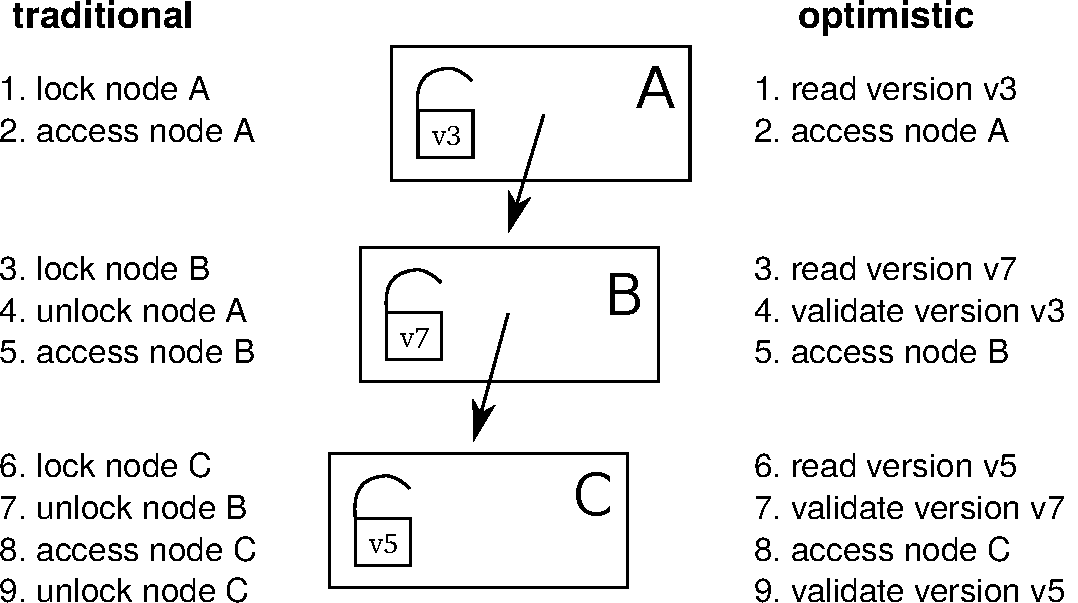
\includegraphics[width=0.65\linewidth]{olcall.pdf}
  \vspace{0.2cm}
  \caption{Comparison of a lookup operation in a 3-level tree using traditional lock coupling (left-hand side) vs.~optimistic lock coupling (right-hand side).}
  \label{fig:olc}
\end{figure}

The traditional and most common lock-based synchronization protocol for B-trees is lock coupling, which interleaves lock acquisitions while holding at most two locks at a time.
If, as we observed earlier, optimistic locks have similar semantics as traditional locks, it is natural to ask whether lock coupling can be combined with optimistic locks.
And indeed the answer is yes: One can almost mechanically translate traditional lock coupling code to optimistic lock coupling code.
This is illustrated in Figure~\ref{fig:olc}, which compares the traversal in a tree of height 3 using traditional and optimistic locks.
As the figure shows, the main difference is that locking is translated to reading the version and that unlocking becomes validation of the previously read version.
This simple change provides efficient lock-free tree traversal without the need to design a complex synchronization protocol.

It is important to emphasize the conceptual simplicity of OLC in comparison to data structures that use custom protocols like the Bw-tree~\cite{DBLP:conf/icde/LevandoskiLS13a}.
To implement lock-free access, the Bw-tree requires an indirection table, delta nodes, complex splitting and merging logic, retry logic, etc.
OLC, on the other hand, can directly be applied to B-trees mostly by adding the appropriate optimistic locking code and without modifying the node layout itself.
Therefore, OpenBw-Tree, an open source implementation of the Bw-tree, requires an order of magnitude more code than a B-tree based on OLC\footnote{Both implementations are available on GitHub: \url{https://github.com/wangziqi2016/index-microbench}}.
Given how difficult it is to develop, validate, and debug lock-free code, simplicity is obviously a major advantage.

\subsection{Correctness Aspects}

\begin{figure}
  % \centering
  %[basicstyle=\normalsize\ttfamily,showstringspaces=false,columns=fullflexible,breaklines=false,breakatwhitespace=true,numbers=none,numberstyle=\small,style=C,keepspaces=true]
\begin{lstlisting}[basicstyle=\ttfamily,language=C++,numbers=left,numberstyle=\small]
std::atomic<BTreeNode*> root;

// search for key in B+tree, returns payload in resultOut
bool lookup(Key key, Value& resultOut) {
   BTreeNode* node = root.load();
   uint64_t nodeVersion = node->readLockOrRestart();
   if (node != root.load()) // make sure the root is still the root
      restart();

   BTreeInner<Key>* parent = nullptr;
   uint64_t parentVersion = 0;

   while (node->isInner()) {
      auto inner = (BTreeInner*)node;

      // unlock parent and make current node the parent
      if (parent)
         parent->readUnlockOrRestart(parentVersion);
      parent = inner;
      parentVersion = nodeVersion;

      // search for next node
      node = inner->findChild(key);
      // validate 'inner' to ensure that 'node' pointer is valid
      inner->checkOrRestart(nodeVersion);
      // now it safe to dereference 'node' pointer (read its version)
      nodeVersion = node->readLockOrRestart();
   }

   // search in leaf and retrieve payload
   auto leaf = (BTreeLeaf*)node;
   bool success = leaf->findValue(key, resultOut);

   // unlock everything
   if (parent)
      parent->readUnlockOrRestart(parentVersion);
   node->readUnlockOrRestart(nodeVersion);

   return success;
}
\end{lstlisting}
  \vspace{0.2cm}
  \caption{B-tree lookup code using OLC. For simplicity, the restart logic is not shown.}
  \label{fig:lookup}
\end{figure}

So far, we have introduced the high-level ideas behind OLC and have stressed its similarity to traditional lock coupling.
Let us now discuss some cases where the close similarity between lock coupling and OLC breaks down.
To make this more concrete, we show the B-tree lookup code in Figure~\ref{fig:lookup}.
In the code, \texttt{readLockOrRestart} reads the lock version and \texttt{readUnlockOrRestart} validates that the read was correct.

One issue with OLC is that any pointer speculatively read from a node may point to invalid memory (if that node is modified concurrently).
Dereferencing such a pointer (e.g., to read its optimistic lock), may cause a segmentation fault or undefined behavior.
In the code shown in Figure~\ref{fig:lookup}, this problem is prevented by the extra check in line 25, which ensures that the read from the node containing the pointer was correct.
Without this additional validation, the code would in line 27 dereference the pointer speculatively read in line 23.
Note that the implementation of \texttt{checkOrRestart} is actually identical to \texttt{readUnlockOrRestart}.
We chose to give it a different name to highlight the fact that this extra check would not be necessary with read/write locks.

Another potential issue with optimistic locks is code that does not terminate.
Code that speculatively accesses a node, like an intra-node binary search, should be written in a way such that it always terminates---even in the presence of concurrent writes.
Otherwise, the validation code that detects the concurrent write will never run.
The binary search of a B-tree, for example, needs to be written in such a way that each comparison makes progress.
For some data structures that do not require loops in the traversal code (like ART) termination is trivially true.

\subsection{Implementation Details}

% implementation, efficiency
To implement an optimistic lock, one can combine the lock and the version counter into a single 64-bit\footnote{Even after subtracting one bit for the lock status, a back-of-the-envelope calculation can show that 63 bits are large enough to never overflow in practice.} word~\cite{artsync}.
A typical read operation will therefore merely consist of reading this version counter atomically.
In C++11 this can be implemented using the \texttt{std::atomic} type.

On x86, atomic reads are cheap because of x86's strong memory order guarantees.
No memory fences are required for sequentially-consistent loads, which are translated (by both GCC and clang) into standard \texttt{MOV} instructions.
Hence, the only effect of \texttt{std::atomic} for loads is preventing instruction re-ordering.
This makes version access and validation cheap.
Acquiring and releasing an optimistic lock in exclusive mode has comparable cost to a traditional lock:
A fairly expensive sequentially-consistent store is needed for acquiring a lock, while a standard \texttt{MOV} suffices for releasing it.
A simple sinlock-based implementation of optimistic locks can be found in the appendix of an earlier paper~\cite{artsync}.

OLC code must be able to handle restarts since validation or lock upgrade can fail due to concurrent writers.
Restarts can easily be implemented by wrapping the data structure operation in a loop (for simplicity not shown in Figure~\ref{fig:lookup}).
Such a loop also enables limiting the number of optimistic retry operations and falling back to pessimistic locking in cases of very heavy contention.
The ability to fall back to traditional locking is a major advantage of OLC in terms of robustness over lock-free approaches, which do not have this option.

In addition to the optimistic shared mode and the exclusive mode, optimistic locks also support a ``shared pessimistic'' mode, which physically acquires the lock in shared mode (allowing multiple concurrent readers but no writers).
This mode is useful for table (or range) scans that touch many tuples on a leaf page (which would otherwise easily abort).
Finally, let us mention that large range scans and table scans, should be broken up into several per-node traversals as is done in the LeanStore~\cite{leanstore} system.

Like all lock-free data structures, but unlike traditional locking and Hardware Transactional Memory~\cite{DBLP:conf/hpca/KarnagelDRLLSL14,DBLP:journals/pvldb/MakreshanskiLS15,htmtkde}, OLC requires care when deleting (and reusing) nodes.
The reason is that a deleting thread can never be sure that a node can be reclaimed because other threads might still be optimistically reading from that node.
Therefore, standard solutions like epoch-based reclamation~\cite{DBLP:conf/sosp/TuZKLM13}, hazard pointers~\cite{DBLP:journals/tpds/Michael04}, or optimized hazard pointers~\cite{DBLP:conf/spaa/BalmauGHZ16} need to be used.
These memory reclamation techniques are, however, largely orthogonal to the synchronization protocol itself.

%-lock-free is not a strong guarantee

\newpage
\section{Evaluation}\label{sec:evaluation}

Let us now experimentally evaluate the overhead and scalability of OLC.
For the experiments, we use an in-memory B+tree implemented in C++11 using templates, which is configured to use nodes of 4096 bytes, random 8 byte keys, and 8 byte payloads.
Based on this B-tree, we compare the following synchronization approaches:
\begin{itemize}
\item an OLC implementation\footnote{An almost identical OLC implementation is available on github: \url{https://github.com/wangziqi2016/index-microbench/tree/master/BTreeOLC}}
\item a variant based on traditional lock coupling and read/write locks
\item the unsynchronized B-tree, which obviously is only correct for read-only workloads but allows measuring the overhead of synchronization
\end{itemize}
Note that earlier work has compared the OLC implementation with a Bw-tree implementation~\cite{buzzword} and other state-of-the-art in-memory index structures.

We use a Haswell EP system with an Intel Xeon E5-2687W v3 CPU, which has 10 cores (20 ``Hyper-Threads'') and 25~MB of L3 cache.
The system is running Ubuntu 18.10 and we use GCC 8.2.0 to compile our code.
The CPU counters are obtained using the Linux perf API\footnote{We use the following convenience wrapper: \url{https://github.com/viktorleis/perfevent}}.

\begin{table}
  \caption{Performance and CPU counters for lookup and insert operations in a B-tree with 100M keys. We perform 100M operations and normalize the CPU counters by that number.}
  \label{tab:overhead}
  \centering
  \begin{tabular}{lrrrrrrr}\toprule
                    &         &        &        & instruc-  & L1     & L3     & branch \\
                    & threads & M op/s & cycles & tions & misses & misses & misses \\\midrule
lookup (no sync.)   & 1       & 1.72   & 2028   & 283     & 39.1   & 14.9   & 16.1   \\
lookup (OLC)        & 1       & 1.65   & 2107   & 370     & 43.9   & 15.1   & 16.7   \\
lookup (lock coup.) & 1       & 1.72   & 2078   & 365     & 42.3   & 16.9   & 15.7   \\\midrule
insert (no sync.)   & 1       & 1.51   & 2286   & 530     & 59.8   & 31.1   & 17.3   \\
insert (OLC)        & 1       & 1.50   & 2303   & 629     & 61.2   & 31.1   & 16.5   \\
insert (lock coup.) & 1       & 1.41   & 2473   & 644     & 61.0   & 31.0   & 17.2   \\\midrule
lookup (no sync.)   & 10      & 15.48  & 2058   & 283     & 38.6   & 15.5   & 16.0   \\
lookup (OLC)        & 10      & 14.60  & 2187   & 370     & 43.8   & 15.8   & 16.8   \\
lookup (lock coup.) & 10      & 5.71   & 5591   & 379     & 54.2   & 17.0   & 14.8   \\\midrule
insert (no sync.)   & 10      & -      & -      & -       & -      & -      & -      \\
insert (OLC)        & 10      & 10.46  & 2940   & 656     & 62.0   & 32.5   & 16.8   \\
insert (lock coup.) & 10      & 7.55   & 4161   & 667     & 75.0   & 28.6   & 16.2   \\
    \bottomrule
\end{tabular}
\end{table}

Table~\ref{tab:overhead} compares the performance and CPU counters for lookup and insert operations in a B-tree with 100M keys.
With {\em single-threaded} execution, we observe that all three approaches have very similar performance.
Adding traditional or optimistic locks to unsynchronized B-tree code results in up to 30\% of additional instructions without affecting single-threaded performance much.

\begin{figure}
  \centering
  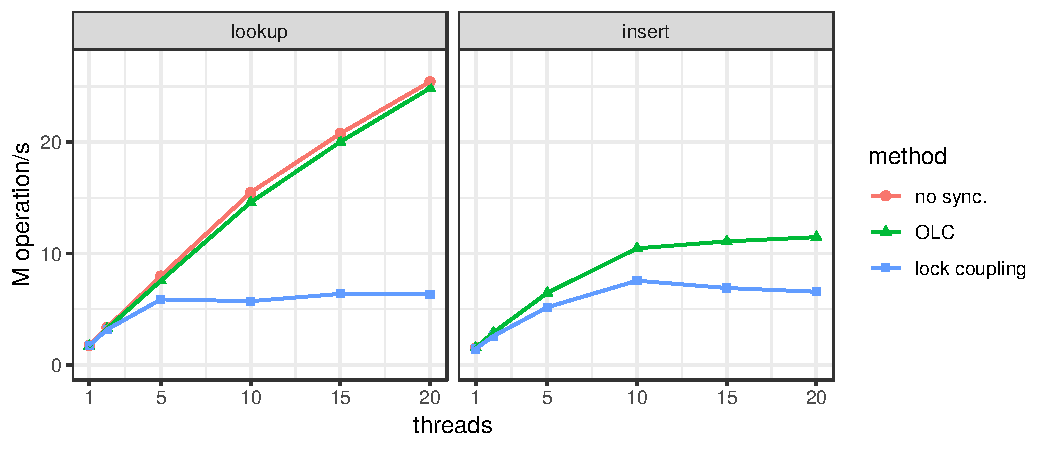
\includegraphics[width=\linewidth]{scale.pdf}
  \vspace{0.2cm}
  \caption{Scalability on 10-core system for B-tree operations (100M values).}
  \label{fig:scale}
\end{figure}

As Figure~\ref{fig:scale} shows, the results change dramatically once we use multiple threads.
For lookup, the scalability of OLC is near-linear up to 20 threads, even though the system has only 10 ``real cores''.
The OLC scalability for insert is also respectable (though not quite as linear because multi-threaded insertion approaches the memory bandwidth of our processor).
The figure also shows that the results of traditional lock coupling with read/write locks are significantly worse than OLC.
With 20 threads, lookup with OLC is 3.9$\times$ faster than traditional lock coupling.

\section{Summary}\label{sec:conc}

Optimistic Lock Coupling (OLC) is an effective synchronization method that combines the simplicity of traditional lock coupling with the superior scalability of lock-free approaches.
OLC is widely applicable and has already been successfully used to synchronize several data structures, including B-trees, binary search trees, and different trie variants.
These features make it highly attractive for modern database systems as well as performance-critical systems software in general.

\begin{thebibliography}{10}

\bibitem{DBLP:conf/spaa/BalmauGHZ16}
O.~Balmau, R.~Guerraoui, M.~Herlihy, and I.~Zablotchi.
\newblock Fast and robust memory reclamation for concurrent data structures.
\newblock In {\em SPAA}, 2016.

\bibitem{DBLP:journals/acta/BayerS77}
R.~Bayer and M.~Schkolnick.
\newblock Concurrency of operations on {B}-trees.
\newblock {\em Acta Informatica}, 9, 1977.

\bibitem{hot}
R.~Binna, E.~Zangerle, M.~Pichl, G.~Specht, and V.~Leis.
\newblock {HOT}: A height optimized trie index for main-memory database
  systems.
\newblock In {\em SIGMOD}, 2018.

\bibitem{DBLP:conf/ppopp/BronsonCCO10}
N.~G. Bronson, J.~Casper, H.~Chafi, and K.~Olukotun.
\newblock A practical concurrent binary search tree.
\newblock In {\em PPOPP}, 2010.

\bibitem{DBLP:conf/vldb/ChaHKK01}
S.~K. Cha, S.~Hwang, K.~Kim, and K.~Kwon.
\newblock Cache-conscious concurrency control of main-memory indexes on
  shared-memory multiprocessor systems.
\newblock In {\em VLDB}, 2001.

\bibitem{intel}
I.~Cutress.
\newblock {Intel} goes for 48-cores: {Cascade-AP} with multi-chip package
  coming soon.
\newblock
  \url{https://www.anandtech.com/show/13535/intel-goes-for-48cores-cascade-ap},
  2018 (accessed January, 2019).

\bibitem{DBLP:conf/cidr/FaleiroA17}
J.~M. Faleiro and D.~J. Abadi.
\newblock Latch-free synchronization in database systems: Silver bullet or
  fool's gold?
\newblock In {\em CIDR}, 2017.

\bibitem{DBLP:journals/ftdb/Graefe11}
G.~Graefe.
\newblock Modern {B}-tree techniques.
\newblock {\em Foundations and Trends in Databases}, 3(4), 2011.

\bibitem{DBLP:conf/hpca/KarnagelDRLLSL14}
T.~Karnagel, R.~Dementiev, R.~Rajwar, K.~Lai, T.~Legler, B.~Schlegel, and
  W.~Lehner.
\newblock Improving in-memory database index performance with
  {Intel}\({}^{\mbox{{\textregistered}}}\) transactional synchronization
  extensions.
\newblock In {\em HPCA}, 2014.

\bibitem{DBLP:journals/tods/LehmanY81}
P.~L. Lehman and S.~B. Yao.
\newblock Efficient locking for concurrent operations on {B}-trees.
\newblock {\em {ACM} Trans. Database Syst.}, 6(4), 1981.

\bibitem{leanstore}
V.~Leis, M.~Haubenschild, A.~Kemper, and T.~Neumann.
\newblock Leanstore: In-memory data management beyond main memory.
\newblock In {\em ICDE}, 2018.

\bibitem{art}
V.~Leis, A.~Kemper, and T.~Neumann.
\newblock The adaptive radix tree: {ARTful} indexing for main-memory databases.
\newblock In {\em ICDE}, 2013.

\bibitem{htmtkde}
V.~Leis, A.~Kemper, and T.~Neumann.
\newblock Scaling {HTM}-supported database transactions to many cores.
\newblock {\em {IEEE} Trans. Knowl. Data Eng.}, 28(2), 2016.

\bibitem{artsync}
V.~Leis, F.~Scheibner, A.~Kemper, and T.~Neumann.
\newblock The {ART} of practical synchronization.
\newblock In {\em DaMoN}, 2016.

\bibitem{DBLP:conf/icde/LevandoskiLS13a}
J.~J. Levandoski, D.~B. Lomet, and S.~Sengupta.
\newblock The {Bw}-tree: A {B}-tree for new hardware platforms.
\newblock In {\em ICDE}, 2013.

\bibitem{DBLP:journals/pvldb/MakreshanskiLS15}
D.~Makreshanski, J.~J. Levandoski, and R.~Stutsman.
\newblock To lock, swap, or elide: On the interplay of hardware transactional
  memory and lock-free indexing.
\newblock {\em {PVLDB}}, 8(11), 2015.

\bibitem{DBLP:dblp_conf/eurosys/MaoKM12}
Y.~Mao, E.~Kohler, and R.~T. Morris.
\newblock Cache craftiness for fast multicore key-value storage.
\newblock In {\em EuroSys}, 2012.

\bibitem{DBLP:journals/tpds/Michael04}
M.~M. Michael.
\newblock Hazard pointers: Safe memory reclamation for lock-free objects.
\newblock {\em {IEEE} Trans. Parallel Distrib. Syst.}, 15(6), 2004.

\bibitem{DBLP:journals/jacm/ShalevS06}
O.~Shalev and N.~Shavit.
\newblock Split-ordered lists: Lock-free extensible hash tables.
\newblock {\em J. {ACM}}, 53(3), 2006.

\bibitem{amd}
A.~Shilov.
\newblock {AMD} previews {EPYC} ‘{Rome}’ processor: Up to 64 {Zen} 2 cores.
\newblock
  \url{https://www.anandtech.com/show/13561/amd-previews-epyc-rome-processor-up-to-64-zen-2-cores},
  2018 (accessed January, 2019).

\bibitem{DBLP:conf/sosp/TuZKLM13}
S.~Tu, W.~Zheng, E.~Kohler, B.~Liskov, and S.~Madden.
\newblock Speedy transactions in multicore in-memory databases.
\newblock In {\em SOSP}, 2013.

\bibitem{buzzword}
Z.~Wang, A.~Pavlo, H.~Lim, V.~Leis, H.~Zhang, M.~Kaminsky, and D.~Andersen.
\newblock Building a {Bw}-tree takes more than just buzz words.
\newblock In {\em SIGMOD}, 2018.

\end{thebibliography}


%\bibliographystyle{abbrv}
%\bibliography{main}

\end{document}

\end{article}

\begin{article}
	{Human-in-the-loop Techniques in Machine Learning}
	{Chengliang Chai, Guoliang Li}
	\pdfminorversion=5
\documentclass[11pt]{article}
\usepackage{deauthor,times,graphicx,caption,microtype}
\usepackage{hyperref}
\usepackage{listings}
\usepackage{booktabs}

\begin{document}

\title{Optimistic Lock Coupling: A Scalable and Efficient General-Purpose Synchronization Method}

\author{Viktor Leis, Michael Haubenschild\raisebox{0.9ex}{$\ast$}, Thomas Neumann\\ Technische Universit{\"a}t M{\"u}nchen \hspace{0.7cm} Tableau Software\raisebox{0.9ex}{$\ast$} \\ {\{leis,neumann\}{@}in.tum.de} \hspace{0.7cm} {mhaubenschild{@}tableau.com\raisebox{0.9ex}{$\ast$}}}

\maketitle

\begin{abstract}
As the number of cores on commodity processors continues to increase, scalability becomes more and more crucial for overall performance.
Scalable and efficient concurrent data structures are particularly important, as these are often the building blocks of parallel algorithms.
Unfortunately, traditional synchronization techniques based on fine-grained locking have been shown to be unscalable on modern multi-core CPUs.
Lock-free data structures, on the other hand, are extremely difficult to design and often incur significant overhead.

In this work, we make the case for Optimistic Lock Coupling as a practical alternative to both traditional locking and the lock-free approach.
We show that Optimistic Lock Coupling is highly scalable and almost as simple to implement as traditional lock coupling.
Another important advantage is that it is easily applicable to most tree-like data structures.
We therefore argue that Optimistic Lock Coupling, rather than a complex and error-prone custom synchronization protocol, should be the default choice for performance-critical data structures.
\end{abstract}

\section{Introduction}

% more and more cores
Today, Intel's commodity server processors have up to 28 cores and its upcoming microarchitecture will have up to 48 cores per socket~\cite{intel}.
Similarly, AMD currently stands at 32 cores and this number is expected to double in the next generation~\cite{amd}.
Since both platforms support simultaneous multithreading (also known as hyperthreading), affordable commodity servers (with up to two sockets) will soon routinely have between 100 and 200 hardware threads.

% data structure scalability is important
With such a high degree of hardware parallelism, efficient data processing crucially depends on how well concurrent data structures scale.
Internally, database systems use a plethora of data structures like table heaps, internal work queues, and, most importantly, index structures.
Any of these can easily become a scalability (and therefore overall performance) bottleneck on many-core CPUs.

% traditional synchronization: fine-grained locks, slow, cache invalidation
Traditionally, database systems synchronize internal data structures using fine-grained reader/writer locks\footnote{In this work, we focus on data structure synchronization rather than high-level transaction semantics and therefore use the term {\em lock} for what would typically be called {\em latch} in the database literature. We thus follow common computer science (rather than database) terminology.}.
Unfortunately, while fine-grained locking makes lock contention unlikely, it still results in bad scalability because lock acquisition and release require writing to shared memory.
Due to the way cache coherency is implemented on modern multi-core CPUs, these writes cause additional cache misses\footnote{The cache coherency protocol ensures that all copies of a cache line on other cores are invalidated before the write can proceed.} and the cache line containing the lock's internal data becomes a point of physical contention.
As a result, any frequently-accessed lock (e.g., the lock of the root node of a B-tree) severely limits scalability.

% lock-free bw-tree: no more latches, but indirections, extremely complex
Lock-free data structures like the Bw-tree~\cite{DBLP:conf/icde/LevandoskiLS13a} (a lock-free B-tree variant) or the Split-Ordered List~\cite{DBLP:journals/jacm/ShalevS06} (a lock-free hash table) do not acquire any locks and therefore generally scale much better than locking-based approaches (in particular for read-mostly workloads).
However, lock-free synchronization has other downsides:
First, it is very difficult and results in extremely complex and error-prone code (when compared to locking).
Second, because the functionality of atomic primitives provided by the hardware (e.g., atomically compare-and-swap 8 bytes) is limited, complex operations require additional indirections within the data structure.
For example, the Bw-tree requires an indirection table and the Split-Ordered List requires ``dummy nodes'', resulting in overhead due to additional cache misses.

% OLC for the win
In this paper we make the case for {\em Optimistic Lock Coupling (OLC)}, a synchronization method that combines some of the best properties of lock-based and lock-free synchronization.
OLC utilizes a special lock type that can be used in two modes:
The first mode is similar to a traditional mutex and excludes other threads by physically acquiring the underlying lock.
In the second mode, reads can proceed optimistically by validating a version counter that is embedded in the lock (similar to optimistic concurrency control).
The first mode is typically used by writers and the second mode by readers.
Besides this special lock type, OLC is based on the observation that optimistic lock validations can be interleaved/coupled---similar to the pair-wise interleaved lock acquisition of traditional lock coupling.
Hence, the name Optimistic Lock Coupling.

OLC has a number of desirable features:
\begin{itemize}
\item By reducing the number of writes to shared memory locations and thereby avoiding cache invalidations, it {\bf scales well} for most workloads.
\item In comparison to unsynchronized code, it requires few additional CPU instructions making it {\bf efficient}.
\item OLC is {\bf widely applicable} to different data structures. It has already been successfully used for synchronizing binary search trees~\cite{DBLP:conf/ppopp/BronsonCCO10}, tries~\cite{artsync}, trie/B-tree hybrids~\cite{DBLP:dblp_conf/eurosys/MaoKM12}, and B-trees~\cite{buzzword}.
\item In comparison to the lock-free paradigm, it is also {\bf easy to use} and requires few modifications to existing, single-threaded data structures.
\end{itemize}
Despite these positive features and its simplicity, OLC is not yet widely known.
The goal of this paper is therefore to popularize this simple idea and to make a case for it.
We argue that OLC deserves to be widely known.
It is a good default synchronization paradigm---more complex, data structure-specific protocols are seldom beneficial.

The rest of the paper is organized as follows.
Section~\ref{sec:related} discusses related work, tracing the history of OLC and its underlying ideas in the literature.
The core of the paper is Section~\ref{sec:olc}, which describes the ideas behind OLC and how it can be used to synchronize complex data structures.
In Section~\ref{sec:evaluation} we experimentally show that OLC has low overhead and scales well when used to synchronize an in-memory B-tree.
We summarize the paper in Section~\ref{sec:conc}.

\newpage
\section{Related Work}\label{sec:related}

Lock coupling has been proposed as a method for allowing concurrent operations on B-trees in 1977~\cite{DBLP:journals/acta/BayerS77}.
This traditional and still widely-used method, described in detail in Graefe's B-tree survey~\cite{DBLP:journals/ftdb/Graefe11}, is also called ``latch coupling'', ``hand-over-hand locking'', and ``crabbing''.
Because at most two locks are held at-a-time during tree traversal, this technique seemingly allows for a high degree of parallelism---in particular if read/write locks are used to enable inner nodes to be locked in shared mode.
However, as we show in Section~\ref{sec:evaluation}, on modern hardware lock acquisition (even in shared mode) results in suboptimal scalability.

An early alternative from 1981 is a B-tree variant called B-link tree~\cite{DBLP:journals/tods/LehmanY81}, which only holds a single lock at a time.
It is based on the observation that between the release of the parent lock and the acquisition of the child lock, the only ``dangerous'' thing that could have happened is the split of a child node (assuming one does not implement merge operations).
Thus, when a split happens, the key being searched might end up on a neighboring node to the right of the current child node.
A B-link tree traversal therefore detects this condition and, if needed, transparently proceeds to the neighboring node.
Releasing the parent lock early is highly beneficial when the child node needs to be fetched from disk.
For in-memory workloads, however, the B-link tree has the same scalability issues as lock coupling (it acquires just as many locks).

The next major advance, Optimistic Latch-Free Index Traversal (OLFIT)~\cite{DBLP:conf/vldb/ChaHKK01}, was proposed in 2001.
OLFIT introduced the idea of a combined lock/update counter, which we call {\em optimistic lock}. % , for lack of a better name,
Based on these per-node optimistic locks and the synchronization protocol of the B-link tree, OLFIT finally achieves good scalability on parallel processors.
The OLFIT protocol is fairly complex, as it requires both the non-trivial B-link protocol and optimistic locks.
Furthermore, like the B-link tree protocol, it does not support merging nodes, and is specific to B-trees (cannot easily be applied to other data structures).

In the following two decades, the growth of main-memory capacity led to much research into other data structures besides the venerable B-tree.
Particularly relevant for our discussion is Bronson et al.'s~\cite{DBLP:conf/ppopp/BronsonCCO10} concurrent binary search tree, which is based on optimistic version validation and has a sophisticated, data structure-specific synchronization protocol.
To the best of our knowledge, this 2010 paper is the first that, as part of its protocol, interleaves version validation across nodes---rather than validating each node separately like OLFIT.
In that paper, this idea is called ``hand-over-hand, optimistic validation'', while we prefer the term Optimistic Lock Coupling to highlight the close resemblance to traditional lock coupling.
Similarly, Mao et al.'s~\cite{DBLP:dblp_conf/eurosys/MaoKM12} Masstree (a concurrent hybrid trie/B-tree) is also based on the same ideas, but again uses them as part of a more complex protocol.

The Adaptive Radix Tree (ART)~\cite{art} is another recent in-memory data structure, which we proposed in 2013.
In contrast to the two data structures just mentioned, it was originally designed with single-threaded performance in mind without supporting concurrency.
To add support for concurrency, we initially started designing a custom protocol called Read-Optimized Write Exclusion (ROWEX)~\cite{artsync}, which turned out to be non-trivial and requires modifications of the underlying data structure\footnote{Note that ROWEX is already easier to apply to existing data structures than the lock-free approach. The difficulty depends on the data structure. Applying ROWEX is hard for B-trees with sorted keys and fairly easy for copy-on-write data structures like the Height Optimized Trie~\cite{hot}---with ART being somewhere in the middle.}.
However, fairly late in the project, we also realized, that OLC {\em alone} (rather than as part of a more complex protocol) is sufficient to synchronize ART.
No other changes to the data structure were necessary.
Both approaches were published and experimentally evaluated in a followup paper~\cite{artsync}, which shows that, despite its simplicity, OLC is efficient, scalable, and generally outperforms ROWEX.

Similar results were recently published regarding B-trees~\cite{buzzword}.
In this experimental study a simple OLC-based synchronization outperformed the Bw-tree~\cite{DBLP:conf/icde/LevandoskiLS13a}, a complex lock-free synchronization approach.
Another recent paper shows that for write-intensive workloads, locking often performs better than lock-free synchronization~\cite{DBLP:conf/cidr/FaleiroA17}.
These experiences indicate that OLC is a general-purpose synchronization paradigm and motivate the current paper.

%foster b-tree\cite{DBLP:journals/tods/GraefeKK12}
%Shasha theory~\cite{DBLP:journals/tods/ShashaG88}

\section{Optimistic Lock Coupling}\label{sec:olc}

% locks suck
The standard technique for inter-thread synchronization is mutual exclusion using fine-grained locks.
In a B-tree, for example, every node usually has its own associated lock, which is acquired before accessing that node.
The problem of locking on modern multi- and many-core processors is that lock acquisition and release require writing to the shared memory location that implements the lock.
This write causes exclusive ownership of the underlying cache line and invalidates copies of it on all other processor cores.
For hierarchical, tree-like data structures, the lock of the root node becomes a point of physical contention---even in read-only workloads and even when read/write locks are used.
Depending on the specific data structure, number of cores, cache coherency protocol implementation, cache topology, whether Non-Uniform Memory Access (NUMA) is used, locking can even result in multi-threaded performance that is worse than single-threaded execution.

% in b-trees this happens very much
The inherent pessimism of locking is particularly unfortunate for B-trees:
Despite the fact that logical modifications of the root node are very infrequent, every B-tree operation must lock the root node during tree traversal\footnote{To a lesser extent this obviously applies to all inner nodes, not just the root.}.
Even the vast majority of update operations (with the exception of splits and merges), only modify a single leaf node.
These observations indicate that a more optimistic approach, which does not require locking inner nodes, would be very beneficial for B-trees.

\subsection{Optimistic Locks}

% optimism to the rescue
As the name indicates, optimistic locks try to solve the scalability issues of traditional locks using an optimistic approach.
Instead of always physically acquiring locks, even for nodes that are unlikely to be modified simultaneously, after-the-fact validation is used to detect conflicts.
This is done by augmenting each lock with a version/update counter that is incremented on every modification.
Using this version counter, readers can optimistically proceed before validating that the version did not change to ensure that the read was safe.
If validation fails, the operation is restarted.

% details on opt locks
Using optimistic locks, a read-only node access (i.e., the majority of all operations in a B-tree) does not acquire the lock and does not increment the version counter.
Instead, it performs the following steps:
\begin{enumerate}
\item read lock version (restart if lock is not free)
\item access node
\item read the version again and validate that it has not changed in the meantime
\end{enumerate}
If the last step (the validation) fails, the operation has to be restarted.
Write operations, on the other hand, are more similar to traditional locking:
\begin{enumerate}
\item acquire lock (wait if necessary)
\item access/write to node
\item increment version and unlock node
\end{enumerate}
Writes can therefore protect a node from other writes.

% similar to locks
As we observed in an earlier paper~\cite{artsync}, because of similar semantics, optimistic locks can be hidden behind an API very similar to traditional read/write locks.
Both approaches have an exclusive lock mode, and acquiring a traditional lock in shared mode is analogous to optimistic version validation.
Furthermore, like with some implementations of traditional read/write locks, optimistic locks allow upgrading a shared lock to an exclusive lock.
Lock upgrades are, for example, used to avoid most B-tree update operations from having to lock inner nodes.
In our experience, the close resemblance of optimistic and traditional locks simplifies the reasoning about optimistic locks;
one can apply similar thinking as in traditional lock-based protocols.

\subsection{Lock Coupling with Optimistic Locks}

\begin{figure}
  \centering
  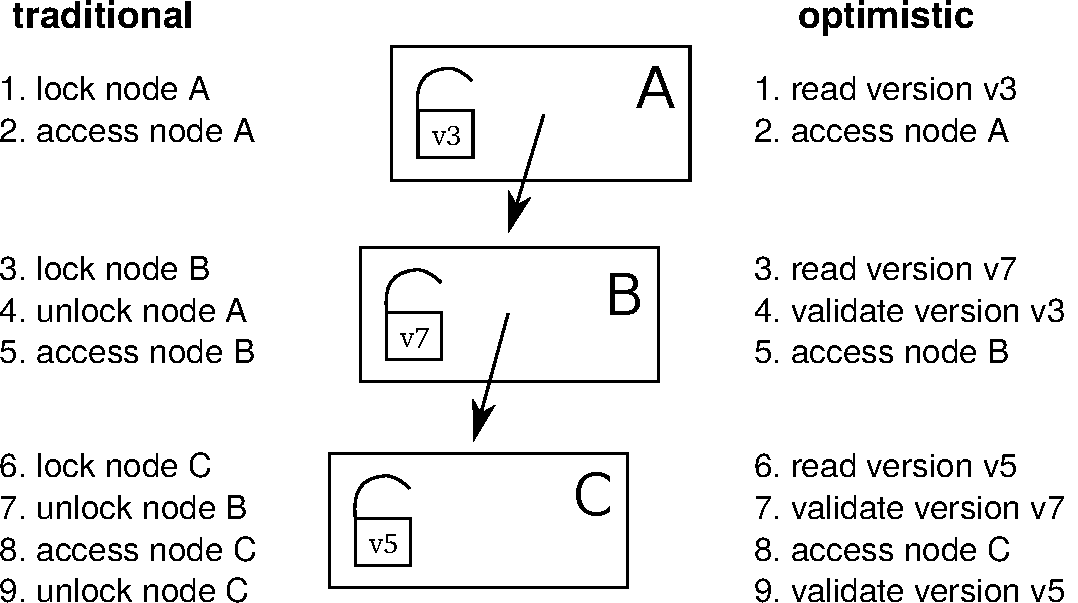
\includegraphics[width=0.65\linewidth]{olcall.pdf}
  \vspace{0.2cm}
  \caption{Comparison of a lookup operation in a 3-level tree using traditional lock coupling (left-hand side) vs.~optimistic lock coupling (right-hand side).}
  \label{fig:olc}
\end{figure}

The traditional and most common lock-based synchronization protocol for B-trees is lock coupling, which interleaves lock acquisitions while holding at most two locks at a time.
If, as we observed earlier, optimistic locks have similar semantics as traditional locks, it is natural to ask whether lock coupling can be combined with optimistic locks.
And indeed the answer is yes: One can almost mechanically translate traditional lock coupling code to optimistic lock coupling code.
This is illustrated in Figure~\ref{fig:olc}, which compares the traversal in a tree of height 3 using traditional and optimistic locks.
As the figure shows, the main difference is that locking is translated to reading the version and that unlocking becomes validation of the previously read version.
This simple change provides efficient lock-free tree traversal without the need to design a complex synchronization protocol.

It is important to emphasize the conceptual simplicity of OLC in comparison to data structures that use custom protocols like the Bw-tree~\cite{DBLP:conf/icde/LevandoskiLS13a}.
To implement lock-free access, the Bw-tree requires an indirection table, delta nodes, complex splitting and merging logic, retry logic, etc.
OLC, on the other hand, can directly be applied to B-trees mostly by adding the appropriate optimistic locking code and without modifying the node layout itself.
Therefore, OpenBw-Tree, an open source implementation of the Bw-tree, requires an order of magnitude more code than a B-tree based on OLC\footnote{Both implementations are available on GitHub: \url{https://github.com/wangziqi2016/index-microbench}}.
Given how difficult it is to develop, validate, and debug lock-free code, simplicity is obviously a major advantage.

\subsection{Correctness Aspects}

\begin{figure}
  % \centering
  %[basicstyle=\normalsize\ttfamily,showstringspaces=false,columns=fullflexible,breaklines=false,breakatwhitespace=true,numbers=none,numberstyle=\small,style=C,keepspaces=true]
\begin{lstlisting}[basicstyle=\ttfamily,language=C++,numbers=left,numberstyle=\small]
std::atomic<BTreeNode*> root;

// search for key in B+tree, returns payload in resultOut
bool lookup(Key key, Value& resultOut) {
   BTreeNode* node = root.load();
   uint64_t nodeVersion = node->readLockOrRestart();
   if (node != root.load()) // make sure the root is still the root
      restart();

   BTreeInner<Key>* parent = nullptr;
   uint64_t parentVersion = 0;

   while (node->isInner()) {
      auto inner = (BTreeInner*)node;

      // unlock parent and make current node the parent
      if (parent)
         parent->readUnlockOrRestart(parentVersion);
      parent = inner;
      parentVersion = nodeVersion;

      // search for next node
      node = inner->findChild(key);
      // validate 'inner' to ensure that 'node' pointer is valid
      inner->checkOrRestart(nodeVersion);
      // now it safe to dereference 'node' pointer (read its version)
      nodeVersion = node->readLockOrRestart();
   }

   // search in leaf and retrieve payload
   auto leaf = (BTreeLeaf*)node;
   bool success = leaf->findValue(key, resultOut);

   // unlock everything
   if (parent)
      parent->readUnlockOrRestart(parentVersion);
   node->readUnlockOrRestart(nodeVersion);

   return success;
}
\end{lstlisting}
  \vspace{0.2cm}
  \caption{B-tree lookup code using OLC. For simplicity, the restart logic is not shown.}
  \label{fig:lookup}
\end{figure}

So far, we have introduced the high-level ideas behind OLC and have stressed its similarity to traditional lock coupling.
Let us now discuss some cases where the close similarity between lock coupling and OLC breaks down.
To make this more concrete, we show the B-tree lookup code in Figure~\ref{fig:lookup}.
In the code, \texttt{readLockOrRestart} reads the lock version and \texttt{readUnlockOrRestart} validates that the read was correct.

One issue with OLC is that any pointer speculatively read from a node may point to invalid memory (if that node is modified concurrently).
Dereferencing such a pointer (e.g., to read its optimistic lock), may cause a segmentation fault or undefined behavior.
In the code shown in Figure~\ref{fig:lookup}, this problem is prevented by the extra check in line 25, which ensures that the read from the node containing the pointer was correct.
Without this additional validation, the code would in line 27 dereference the pointer speculatively read in line 23.
Note that the implementation of \texttt{checkOrRestart} is actually identical to \texttt{readUnlockOrRestart}.
We chose to give it a different name to highlight the fact that this extra check would not be necessary with read/write locks.

Another potential issue with optimistic locks is code that does not terminate.
Code that speculatively accesses a node, like an intra-node binary search, should be written in a way such that it always terminates---even in the presence of concurrent writes.
Otherwise, the validation code that detects the concurrent write will never run.
The binary search of a B-tree, for example, needs to be written in such a way that each comparison makes progress.
For some data structures that do not require loops in the traversal code (like ART) termination is trivially true.

\subsection{Implementation Details}

% implementation, efficiency
To implement an optimistic lock, one can combine the lock and the version counter into a single 64-bit\footnote{Even after subtracting one bit for the lock status, a back-of-the-envelope calculation can show that 63 bits are large enough to never overflow in practice.} word~\cite{artsync}.
A typical read operation will therefore merely consist of reading this version counter atomically.
In C++11 this can be implemented using the \texttt{std::atomic} type.

On x86, atomic reads are cheap because of x86's strong memory order guarantees.
No memory fences are required for sequentially-consistent loads, which are translated (by both GCC and clang) into standard \texttt{MOV} instructions.
Hence, the only effect of \texttt{std::atomic} for loads is preventing instruction re-ordering.
This makes version access and validation cheap.
Acquiring and releasing an optimistic lock in exclusive mode has comparable cost to a traditional lock:
A fairly expensive sequentially-consistent store is needed for acquiring a lock, while a standard \texttt{MOV} suffices for releasing it.
A simple sinlock-based implementation of optimistic locks can be found in the appendix of an earlier paper~\cite{artsync}.

OLC code must be able to handle restarts since validation or lock upgrade can fail due to concurrent writers.
Restarts can easily be implemented by wrapping the data structure operation in a loop (for simplicity not shown in Figure~\ref{fig:lookup}).
Such a loop also enables limiting the number of optimistic retry operations and falling back to pessimistic locking in cases of very heavy contention.
The ability to fall back to traditional locking is a major advantage of OLC in terms of robustness over lock-free approaches, which do not have this option.

In addition to the optimistic shared mode and the exclusive mode, optimistic locks also support a ``shared pessimistic'' mode, which physically acquires the lock in shared mode (allowing multiple concurrent readers but no writers).
This mode is useful for table (or range) scans that touch many tuples on a leaf page (which would otherwise easily abort).
Finally, let us mention that large range scans and table scans, should be broken up into several per-node traversals as is done in the LeanStore~\cite{leanstore} system.

Like all lock-free data structures, but unlike traditional locking and Hardware Transactional Memory~\cite{DBLP:conf/hpca/KarnagelDRLLSL14,DBLP:journals/pvldb/MakreshanskiLS15,htmtkde}, OLC requires care when deleting (and reusing) nodes.
The reason is that a deleting thread can never be sure that a node can be reclaimed because other threads might still be optimistically reading from that node.
Therefore, standard solutions like epoch-based reclamation~\cite{DBLP:conf/sosp/TuZKLM13}, hazard pointers~\cite{DBLP:journals/tpds/Michael04}, or optimized hazard pointers~\cite{DBLP:conf/spaa/BalmauGHZ16} need to be used.
These memory reclamation techniques are, however, largely orthogonal to the synchronization protocol itself.

%-lock-free is not a strong guarantee

\newpage
\section{Evaluation}\label{sec:evaluation}

Let us now experimentally evaluate the overhead and scalability of OLC.
For the experiments, we use an in-memory B+tree implemented in C++11 using templates, which is configured to use nodes of 4096 bytes, random 8 byte keys, and 8 byte payloads.
Based on this B-tree, we compare the following synchronization approaches:
\begin{itemize}
\item an OLC implementation\footnote{An almost identical OLC implementation is available on github: \url{https://github.com/wangziqi2016/index-microbench/tree/master/BTreeOLC}}
\item a variant based on traditional lock coupling and read/write locks
\item the unsynchronized B-tree, which obviously is only correct for read-only workloads but allows measuring the overhead of synchronization
\end{itemize}
Note that earlier work has compared the OLC implementation with a Bw-tree implementation~\cite{buzzword} and other state-of-the-art in-memory index structures.

We use a Haswell EP system with an Intel Xeon E5-2687W v3 CPU, which has 10 cores (20 ``Hyper-Threads'') and 25~MB of L3 cache.
The system is running Ubuntu 18.10 and we use GCC 8.2.0 to compile our code.
The CPU counters are obtained using the Linux perf API\footnote{We use the following convenience wrapper: \url{https://github.com/viktorleis/perfevent}}.

\begin{table}
  \caption{Performance and CPU counters for lookup and insert operations in a B-tree with 100M keys. We perform 100M operations and normalize the CPU counters by that number.}
  \label{tab:overhead}
  \centering
  \begin{tabular}{lrrrrrrr}\toprule
                    &         &        &        & instruc-  & L1     & L3     & branch \\
                    & threads & M op/s & cycles & tions & misses & misses & misses \\\midrule
lookup (no sync.)   & 1       & 1.72   & 2028   & 283     & 39.1   & 14.9   & 16.1   \\
lookup (OLC)        & 1       & 1.65   & 2107   & 370     & 43.9   & 15.1   & 16.7   \\
lookup (lock coup.) & 1       & 1.72   & 2078   & 365     & 42.3   & 16.9   & 15.7   \\\midrule
insert (no sync.)   & 1       & 1.51   & 2286   & 530     & 59.8   & 31.1   & 17.3   \\
insert (OLC)        & 1       & 1.50   & 2303   & 629     & 61.2   & 31.1   & 16.5   \\
insert (lock coup.) & 1       & 1.41   & 2473   & 644     & 61.0   & 31.0   & 17.2   \\\midrule
lookup (no sync.)   & 10      & 15.48  & 2058   & 283     & 38.6   & 15.5   & 16.0   \\
lookup (OLC)        & 10      & 14.60  & 2187   & 370     & 43.8   & 15.8   & 16.8   \\
lookup (lock coup.) & 10      & 5.71   & 5591   & 379     & 54.2   & 17.0   & 14.8   \\\midrule
insert (no sync.)   & 10      & -      & -      & -       & -      & -      & -      \\
insert (OLC)        & 10      & 10.46  & 2940   & 656     & 62.0   & 32.5   & 16.8   \\
insert (lock coup.) & 10      & 7.55   & 4161   & 667     & 75.0   & 28.6   & 16.2   \\
    \bottomrule
\end{tabular}
\end{table}

Table~\ref{tab:overhead} compares the performance and CPU counters for lookup and insert operations in a B-tree with 100M keys.
With {\em single-threaded} execution, we observe that all three approaches have very similar performance.
Adding traditional or optimistic locks to unsynchronized B-tree code results in up to 30\% of additional instructions without affecting single-threaded performance much.

\begin{figure}
  \centering
  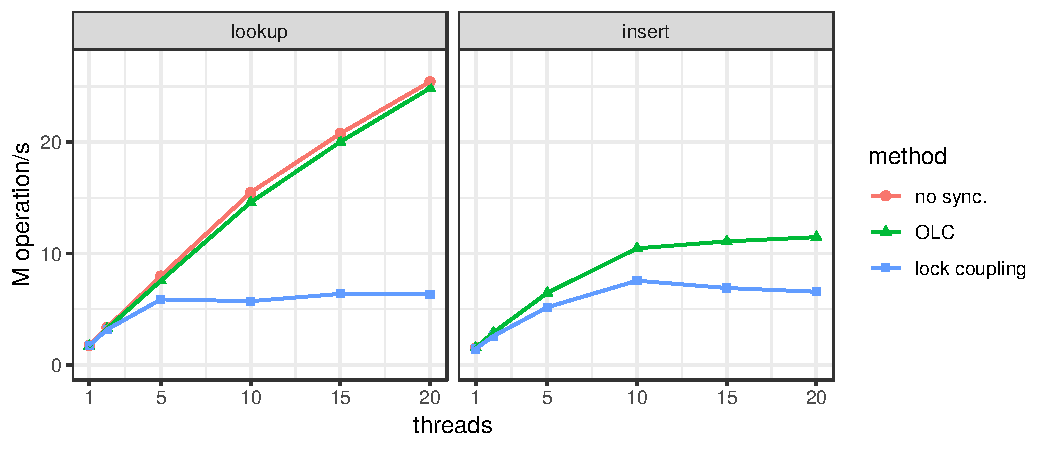
\includegraphics[width=\linewidth]{scale.pdf}
  \vspace{0.2cm}
  \caption{Scalability on 10-core system for B-tree operations (100M values).}
  \label{fig:scale}
\end{figure}

As Figure~\ref{fig:scale} shows, the results change dramatically once we use multiple threads.
For lookup, the scalability of OLC is near-linear up to 20 threads, even though the system has only 10 ``real cores''.
The OLC scalability for insert is also respectable (though not quite as linear because multi-threaded insertion approaches the memory bandwidth of our processor).
The figure also shows that the results of traditional lock coupling with read/write locks are significantly worse than OLC.
With 20 threads, lookup with OLC is 3.9$\times$ faster than traditional lock coupling.

\section{Summary}\label{sec:conc}

Optimistic Lock Coupling (OLC) is an effective synchronization method that combines the simplicity of traditional lock coupling with the superior scalability of lock-free approaches.
OLC is widely applicable and has already been successfully used to synchronize several data structures, including B-trees, binary search trees, and different trie variants.
These features make it highly attractive for modern database systems as well as performance-critical systems software in general.

\begin{thebibliography}{10}

\bibitem{DBLP:conf/spaa/BalmauGHZ16}
O.~Balmau, R.~Guerraoui, M.~Herlihy, and I.~Zablotchi.
\newblock Fast and robust memory reclamation for concurrent data structures.
\newblock In {\em SPAA}, 2016.

\bibitem{DBLP:journals/acta/BayerS77}
R.~Bayer and M.~Schkolnick.
\newblock Concurrency of operations on {B}-trees.
\newblock {\em Acta Informatica}, 9, 1977.

\bibitem{hot}
R.~Binna, E.~Zangerle, M.~Pichl, G.~Specht, and V.~Leis.
\newblock {HOT}: A height optimized trie index for main-memory database
  systems.
\newblock In {\em SIGMOD}, 2018.

\bibitem{DBLP:conf/ppopp/BronsonCCO10}
N.~G. Bronson, J.~Casper, H.~Chafi, and K.~Olukotun.
\newblock A practical concurrent binary search tree.
\newblock In {\em PPOPP}, 2010.

\bibitem{DBLP:conf/vldb/ChaHKK01}
S.~K. Cha, S.~Hwang, K.~Kim, and K.~Kwon.
\newblock Cache-conscious concurrency control of main-memory indexes on
  shared-memory multiprocessor systems.
\newblock In {\em VLDB}, 2001.

\bibitem{intel}
I.~Cutress.
\newblock {Intel} goes for 48-cores: {Cascade-AP} with multi-chip package
  coming soon.
\newblock
  \url{https://www.anandtech.com/show/13535/intel-goes-for-48cores-cascade-ap},
  2018 (accessed January, 2019).

\bibitem{DBLP:conf/cidr/FaleiroA17}
J.~M. Faleiro and D.~J. Abadi.
\newblock Latch-free synchronization in database systems: Silver bullet or
  fool's gold?
\newblock In {\em CIDR}, 2017.

\bibitem{DBLP:journals/ftdb/Graefe11}
G.~Graefe.
\newblock Modern {B}-tree techniques.
\newblock {\em Foundations and Trends in Databases}, 3(4), 2011.

\bibitem{DBLP:conf/hpca/KarnagelDRLLSL14}
T.~Karnagel, R.~Dementiev, R.~Rajwar, K.~Lai, T.~Legler, B.~Schlegel, and
  W.~Lehner.
\newblock Improving in-memory database index performance with
  {Intel}\({}^{\mbox{{\textregistered}}}\) transactional synchronization
  extensions.
\newblock In {\em HPCA}, 2014.

\bibitem{DBLP:journals/tods/LehmanY81}
P.~L. Lehman and S.~B. Yao.
\newblock Efficient locking for concurrent operations on {B}-trees.
\newblock {\em {ACM} Trans. Database Syst.}, 6(4), 1981.

\bibitem{leanstore}
V.~Leis, M.~Haubenschild, A.~Kemper, and T.~Neumann.
\newblock Leanstore: In-memory data management beyond main memory.
\newblock In {\em ICDE}, 2018.

\bibitem{art}
V.~Leis, A.~Kemper, and T.~Neumann.
\newblock The adaptive radix tree: {ARTful} indexing for main-memory databases.
\newblock In {\em ICDE}, 2013.

\bibitem{htmtkde}
V.~Leis, A.~Kemper, and T.~Neumann.
\newblock Scaling {HTM}-supported database transactions to many cores.
\newblock {\em {IEEE} Trans. Knowl. Data Eng.}, 28(2), 2016.

\bibitem{artsync}
V.~Leis, F.~Scheibner, A.~Kemper, and T.~Neumann.
\newblock The {ART} of practical synchronization.
\newblock In {\em DaMoN}, 2016.

\bibitem{DBLP:conf/icde/LevandoskiLS13a}
J.~J. Levandoski, D.~B. Lomet, and S.~Sengupta.
\newblock The {Bw}-tree: A {B}-tree for new hardware platforms.
\newblock In {\em ICDE}, 2013.

\bibitem{DBLP:journals/pvldb/MakreshanskiLS15}
D.~Makreshanski, J.~J. Levandoski, and R.~Stutsman.
\newblock To lock, swap, or elide: On the interplay of hardware transactional
  memory and lock-free indexing.
\newblock {\em {PVLDB}}, 8(11), 2015.

\bibitem{DBLP:dblp_conf/eurosys/MaoKM12}
Y.~Mao, E.~Kohler, and R.~T. Morris.
\newblock Cache craftiness for fast multicore key-value storage.
\newblock In {\em EuroSys}, 2012.

\bibitem{DBLP:journals/tpds/Michael04}
M.~M. Michael.
\newblock Hazard pointers: Safe memory reclamation for lock-free objects.
\newblock {\em {IEEE} Trans. Parallel Distrib. Syst.}, 15(6), 2004.

\bibitem{DBLP:journals/jacm/ShalevS06}
O.~Shalev and N.~Shavit.
\newblock Split-ordered lists: Lock-free extensible hash tables.
\newblock {\em J. {ACM}}, 53(3), 2006.

\bibitem{amd}
A.~Shilov.
\newblock {AMD} previews {EPYC} ‘{Rome}’ processor: Up to 64 {Zen} 2 cores.
\newblock
  \url{https://www.anandtech.com/show/13561/amd-previews-epyc-rome-processor-up-to-64-zen-2-cores},
  2018 (accessed January, 2019).

\bibitem{DBLP:conf/sosp/TuZKLM13}
S.~Tu, W.~Zheng, E.~Kohler, B.~Liskov, and S.~Madden.
\newblock Speedy transactions in multicore in-memory databases.
\newblock In {\em SOSP}, 2013.

\bibitem{buzzword}
Z.~Wang, A.~Pavlo, H.~Lim, V.~Leis, H.~Zhang, M.~Kaminsky, and D.~Andersen.
\newblock Building a {Bw}-tree takes more than just buzz words.
\newblock In {\em SIGMOD}, 2018.

\end{thebibliography}


%\bibliographystyle{abbrv}
%\bibliography{main}

\end{document}

\end{article}

\begin{article}
		{An ML-Powered Human Behavior Management System}
		{Sihem Amer-Yahia, Reynold Cheng, Mohamed Bouadi,
			Abdelouahab Chibah, Mohammadreza Esfandiari, 
			Jiangping Zhou, Nan Zhang, Eric Lau,Yuguo Li,
			Xiaolin Han, Shivansh Mittal
		}
		\pdfminorversion=5
\documentclass[11pt]{article}
\usepackage{deauthor,times,graphicx,caption,microtype}
\usepackage{hyperref}
\usepackage{listings}
\usepackage{booktabs}

\begin{document}

\title{Optimistic Lock Coupling: A Scalable and Efficient General-Purpose Synchronization Method}

\author{Viktor Leis, Michael Haubenschild\raisebox{0.9ex}{$\ast$}, Thomas Neumann\\ Technische Universit{\"a}t M{\"u}nchen \hspace{0.7cm} Tableau Software\raisebox{0.9ex}{$\ast$} \\ {\{leis,neumann\}{@}in.tum.de} \hspace{0.7cm} {mhaubenschild{@}tableau.com\raisebox{0.9ex}{$\ast$}}}

\maketitle

\begin{abstract}
As the number of cores on commodity processors continues to increase, scalability becomes more and more crucial for overall performance.
Scalable and efficient concurrent data structures are particularly important, as these are often the building blocks of parallel algorithms.
Unfortunately, traditional synchronization techniques based on fine-grained locking have been shown to be unscalable on modern multi-core CPUs.
Lock-free data structures, on the other hand, are extremely difficult to design and often incur significant overhead.

In this work, we make the case for Optimistic Lock Coupling as a practical alternative to both traditional locking and the lock-free approach.
We show that Optimistic Lock Coupling is highly scalable and almost as simple to implement as traditional lock coupling.
Another important advantage is that it is easily applicable to most tree-like data structures.
We therefore argue that Optimistic Lock Coupling, rather than a complex and error-prone custom synchronization protocol, should be the default choice for performance-critical data structures.
\end{abstract}

\section{Introduction}

% more and more cores
Today, Intel's commodity server processors have up to 28 cores and its upcoming microarchitecture will have up to 48 cores per socket~\cite{intel}.
Similarly, AMD currently stands at 32 cores and this number is expected to double in the next generation~\cite{amd}.
Since both platforms support simultaneous multithreading (also known as hyperthreading), affordable commodity servers (with up to two sockets) will soon routinely have between 100 and 200 hardware threads.

% data structure scalability is important
With such a high degree of hardware parallelism, efficient data processing crucially depends on how well concurrent data structures scale.
Internally, database systems use a plethora of data structures like table heaps, internal work queues, and, most importantly, index structures.
Any of these can easily become a scalability (and therefore overall performance) bottleneck on many-core CPUs.

% traditional synchronization: fine-grained locks, slow, cache invalidation
Traditionally, database systems synchronize internal data structures using fine-grained reader/writer locks\footnote{In this work, we focus on data structure synchronization rather than high-level transaction semantics and therefore use the term {\em lock} for what would typically be called {\em latch} in the database literature. We thus follow common computer science (rather than database) terminology.}.
Unfortunately, while fine-grained locking makes lock contention unlikely, it still results in bad scalability because lock acquisition and release require writing to shared memory.
Due to the way cache coherency is implemented on modern multi-core CPUs, these writes cause additional cache misses\footnote{The cache coherency protocol ensures that all copies of a cache line on other cores are invalidated before the write can proceed.} and the cache line containing the lock's internal data becomes a point of physical contention.
As a result, any frequently-accessed lock (e.g., the lock of the root node of a B-tree) severely limits scalability.

% lock-free bw-tree: no more latches, but indirections, extremely complex
Lock-free data structures like the Bw-tree~\cite{DBLP:conf/icde/LevandoskiLS13a} (a lock-free B-tree variant) or the Split-Ordered List~\cite{DBLP:journals/jacm/ShalevS06} (a lock-free hash table) do not acquire any locks and therefore generally scale much better than locking-based approaches (in particular for read-mostly workloads).
However, lock-free synchronization has other downsides:
First, it is very difficult and results in extremely complex and error-prone code (when compared to locking).
Second, because the functionality of atomic primitives provided by the hardware (e.g., atomically compare-and-swap 8 bytes) is limited, complex operations require additional indirections within the data structure.
For example, the Bw-tree requires an indirection table and the Split-Ordered List requires ``dummy nodes'', resulting in overhead due to additional cache misses.

% OLC for the win
In this paper we make the case for {\em Optimistic Lock Coupling (OLC)}, a synchronization method that combines some of the best properties of lock-based and lock-free synchronization.
OLC utilizes a special lock type that can be used in two modes:
The first mode is similar to a traditional mutex and excludes other threads by physically acquiring the underlying lock.
In the second mode, reads can proceed optimistically by validating a version counter that is embedded in the lock (similar to optimistic concurrency control).
The first mode is typically used by writers and the second mode by readers.
Besides this special lock type, OLC is based on the observation that optimistic lock validations can be interleaved/coupled---similar to the pair-wise interleaved lock acquisition of traditional lock coupling.
Hence, the name Optimistic Lock Coupling.

OLC has a number of desirable features:
\begin{itemize}
\item By reducing the number of writes to shared memory locations and thereby avoiding cache invalidations, it {\bf scales well} for most workloads.
\item In comparison to unsynchronized code, it requires few additional CPU instructions making it {\bf efficient}.
\item OLC is {\bf widely applicable} to different data structures. It has already been successfully used for synchronizing binary search trees~\cite{DBLP:conf/ppopp/BronsonCCO10}, tries~\cite{artsync}, trie/B-tree hybrids~\cite{DBLP:dblp_conf/eurosys/MaoKM12}, and B-trees~\cite{buzzword}.
\item In comparison to the lock-free paradigm, it is also {\bf easy to use} and requires few modifications to existing, single-threaded data structures.
\end{itemize}
Despite these positive features and its simplicity, OLC is not yet widely known.
The goal of this paper is therefore to popularize this simple idea and to make a case for it.
We argue that OLC deserves to be widely known.
It is a good default synchronization paradigm---more complex, data structure-specific protocols are seldom beneficial.

The rest of the paper is organized as follows.
Section~\ref{sec:related} discusses related work, tracing the history of OLC and its underlying ideas in the literature.
The core of the paper is Section~\ref{sec:olc}, which describes the ideas behind OLC and how it can be used to synchronize complex data structures.
In Section~\ref{sec:evaluation} we experimentally show that OLC has low overhead and scales well when used to synchronize an in-memory B-tree.
We summarize the paper in Section~\ref{sec:conc}.

\newpage
\section{Related Work}\label{sec:related}

Lock coupling has been proposed as a method for allowing concurrent operations on B-trees in 1977~\cite{DBLP:journals/acta/BayerS77}.
This traditional and still widely-used method, described in detail in Graefe's B-tree survey~\cite{DBLP:journals/ftdb/Graefe11}, is also called ``latch coupling'', ``hand-over-hand locking'', and ``crabbing''.
Because at most two locks are held at-a-time during tree traversal, this technique seemingly allows for a high degree of parallelism---in particular if read/write locks are used to enable inner nodes to be locked in shared mode.
However, as we show in Section~\ref{sec:evaluation}, on modern hardware lock acquisition (even in shared mode) results in suboptimal scalability.

An early alternative from 1981 is a B-tree variant called B-link tree~\cite{DBLP:journals/tods/LehmanY81}, which only holds a single lock at a time.
It is based on the observation that between the release of the parent lock and the acquisition of the child lock, the only ``dangerous'' thing that could have happened is the split of a child node (assuming one does not implement merge operations).
Thus, when a split happens, the key being searched might end up on a neighboring node to the right of the current child node.
A B-link tree traversal therefore detects this condition and, if needed, transparently proceeds to the neighboring node.
Releasing the parent lock early is highly beneficial when the child node needs to be fetched from disk.
For in-memory workloads, however, the B-link tree has the same scalability issues as lock coupling (it acquires just as many locks).

The next major advance, Optimistic Latch-Free Index Traversal (OLFIT)~\cite{DBLP:conf/vldb/ChaHKK01}, was proposed in 2001.
OLFIT introduced the idea of a combined lock/update counter, which we call {\em optimistic lock}. % , for lack of a better name,
Based on these per-node optimistic locks and the synchronization protocol of the B-link tree, OLFIT finally achieves good scalability on parallel processors.
The OLFIT protocol is fairly complex, as it requires both the non-trivial B-link protocol and optimistic locks.
Furthermore, like the B-link tree protocol, it does not support merging nodes, and is specific to B-trees (cannot easily be applied to other data structures).

In the following two decades, the growth of main-memory capacity led to much research into other data structures besides the venerable B-tree.
Particularly relevant for our discussion is Bronson et al.'s~\cite{DBLP:conf/ppopp/BronsonCCO10} concurrent binary search tree, which is based on optimistic version validation and has a sophisticated, data structure-specific synchronization protocol.
To the best of our knowledge, this 2010 paper is the first that, as part of its protocol, interleaves version validation across nodes---rather than validating each node separately like OLFIT.
In that paper, this idea is called ``hand-over-hand, optimistic validation'', while we prefer the term Optimistic Lock Coupling to highlight the close resemblance to traditional lock coupling.
Similarly, Mao et al.'s~\cite{DBLP:dblp_conf/eurosys/MaoKM12} Masstree (a concurrent hybrid trie/B-tree) is also based on the same ideas, but again uses them as part of a more complex protocol.

The Adaptive Radix Tree (ART)~\cite{art} is another recent in-memory data structure, which we proposed in 2013.
In contrast to the two data structures just mentioned, it was originally designed with single-threaded performance in mind without supporting concurrency.
To add support for concurrency, we initially started designing a custom protocol called Read-Optimized Write Exclusion (ROWEX)~\cite{artsync}, which turned out to be non-trivial and requires modifications of the underlying data structure\footnote{Note that ROWEX is already easier to apply to existing data structures than the lock-free approach. The difficulty depends on the data structure. Applying ROWEX is hard for B-trees with sorted keys and fairly easy for copy-on-write data structures like the Height Optimized Trie~\cite{hot}---with ART being somewhere in the middle.}.
However, fairly late in the project, we also realized, that OLC {\em alone} (rather than as part of a more complex protocol) is sufficient to synchronize ART.
No other changes to the data structure were necessary.
Both approaches were published and experimentally evaluated in a followup paper~\cite{artsync}, which shows that, despite its simplicity, OLC is efficient, scalable, and generally outperforms ROWEX.

Similar results were recently published regarding B-trees~\cite{buzzword}.
In this experimental study a simple OLC-based synchronization outperformed the Bw-tree~\cite{DBLP:conf/icde/LevandoskiLS13a}, a complex lock-free synchronization approach.
Another recent paper shows that for write-intensive workloads, locking often performs better than lock-free synchronization~\cite{DBLP:conf/cidr/FaleiroA17}.
These experiences indicate that OLC is a general-purpose synchronization paradigm and motivate the current paper.

%foster b-tree\cite{DBLP:journals/tods/GraefeKK12}
%Shasha theory~\cite{DBLP:journals/tods/ShashaG88}

\section{Optimistic Lock Coupling}\label{sec:olc}

% locks suck
The standard technique for inter-thread synchronization is mutual exclusion using fine-grained locks.
In a B-tree, for example, every node usually has its own associated lock, which is acquired before accessing that node.
The problem of locking on modern multi- and many-core processors is that lock acquisition and release require writing to the shared memory location that implements the lock.
This write causes exclusive ownership of the underlying cache line and invalidates copies of it on all other processor cores.
For hierarchical, tree-like data structures, the lock of the root node becomes a point of physical contention---even in read-only workloads and even when read/write locks are used.
Depending on the specific data structure, number of cores, cache coherency protocol implementation, cache topology, whether Non-Uniform Memory Access (NUMA) is used, locking can even result in multi-threaded performance that is worse than single-threaded execution.

% in b-trees this happens very much
The inherent pessimism of locking is particularly unfortunate for B-trees:
Despite the fact that logical modifications of the root node are very infrequent, every B-tree operation must lock the root node during tree traversal\footnote{To a lesser extent this obviously applies to all inner nodes, not just the root.}.
Even the vast majority of update operations (with the exception of splits and merges), only modify a single leaf node.
These observations indicate that a more optimistic approach, which does not require locking inner nodes, would be very beneficial for B-trees.

\subsection{Optimistic Locks}

% optimism to the rescue
As the name indicates, optimistic locks try to solve the scalability issues of traditional locks using an optimistic approach.
Instead of always physically acquiring locks, even for nodes that are unlikely to be modified simultaneously, after-the-fact validation is used to detect conflicts.
This is done by augmenting each lock with a version/update counter that is incremented on every modification.
Using this version counter, readers can optimistically proceed before validating that the version did not change to ensure that the read was safe.
If validation fails, the operation is restarted.

% details on opt locks
Using optimistic locks, a read-only node access (i.e., the majority of all operations in a B-tree) does not acquire the lock and does not increment the version counter.
Instead, it performs the following steps:
\begin{enumerate}
\item read lock version (restart if lock is not free)
\item access node
\item read the version again and validate that it has not changed in the meantime
\end{enumerate}
If the last step (the validation) fails, the operation has to be restarted.
Write operations, on the other hand, are more similar to traditional locking:
\begin{enumerate}
\item acquire lock (wait if necessary)
\item access/write to node
\item increment version and unlock node
\end{enumerate}
Writes can therefore protect a node from other writes.

% similar to locks
As we observed in an earlier paper~\cite{artsync}, because of similar semantics, optimistic locks can be hidden behind an API very similar to traditional read/write locks.
Both approaches have an exclusive lock mode, and acquiring a traditional lock in shared mode is analogous to optimistic version validation.
Furthermore, like with some implementations of traditional read/write locks, optimistic locks allow upgrading a shared lock to an exclusive lock.
Lock upgrades are, for example, used to avoid most B-tree update operations from having to lock inner nodes.
In our experience, the close resemblance of optimistic and traditional locks simplifies the reasoning about optimistic locks;
one can apply similar thinking as in traditional lock-based protocols.

\subsection{Lock Coupling with Optimistic Locks}

\begin{figure}
  \centering
  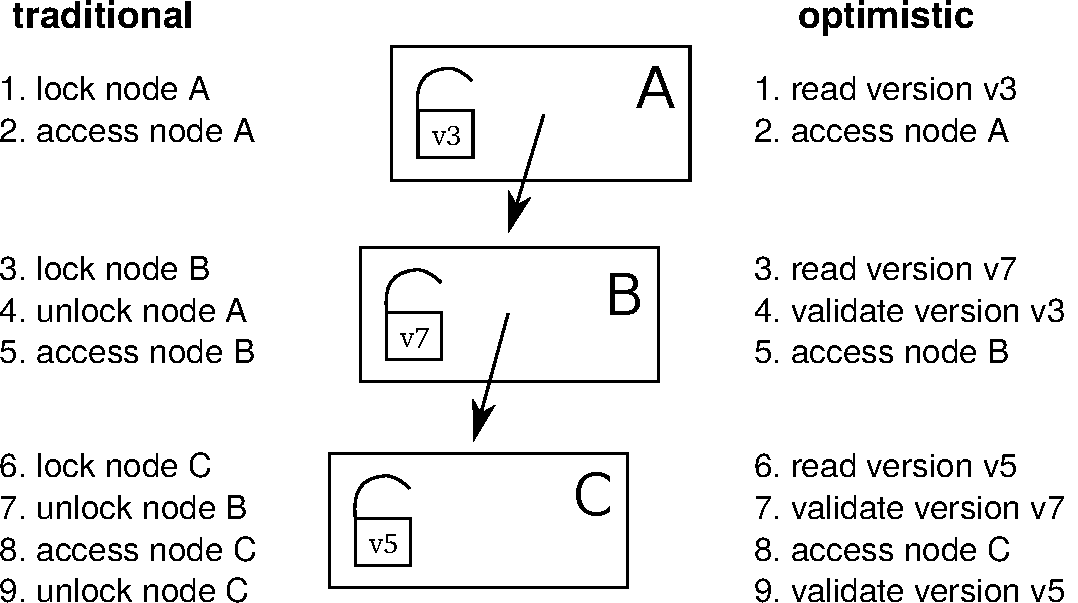
\includegraphics[width=0.65\linewidth]{olcall.pdf}
  \vspace{0.2cm}
  \caption{Comparison of a lookup operation in a 3-level tree using traditional lock coupling (left-hand side) vs.~optimistic lock coupling (right-hand side).}
  \label{fig:olc}
\end{figure}

The traditional and most common lock-based synchronization protocol for B-trees is lock coupling, which interleaves lock acquisitions while holding at most two locks at a time.
If, as we observed earlier, optimistic locks have similar semantics as traditional locks, it is natural to ask whether lock coupling can be combined with optimistic locks.
And indeed the answer is yes: One can almost mechanically translate traditional lock coupling code to optimistic lock coupling code.
This is illustrated in Figure~\ref{fig:olc}, which compares the traversal in a tree of height 3 using traditional and optimistic locks.
As the figure shows, the main difference is that locking is translated to reading the version and that unlocking becomes validation of the previously read version.
This simple change provides efficient lock-free tree traversal without the need to design a complex synchronization protocol.

It is important to emphasize the conceptual simplicity of OLC in comparison to data structures that use custom protocols like the Bw-tree~\cite{DBLP:conf/icde/LevandoskiLS13a}.
To implement lock-free access, the Bw-tree requires an indirection table, delta nodes, complex splitting and merging logic, retry logic, etc.
OLC, on the other hand, can directly be applied to B-trees mostly by adding the appropriate optimistic locking code and without modifying the node layout itself.
Therefore, OpenBw-Tree, an open source implementation of the Bw-tree, requires an order of magnitude more code than a B-tree based on OLC\footnote{Both implementations are available on GitHub: \url{https://github.com/wangziqi2016/index-microbench}}.
Given how difficult it is to develop, validate, and debug lock-free code, simplicity is obviously a major advantage.

\subsection{Correctness Aspects}

\begin{figure}
  % \centering
  %[basicstyle=\normalsize\ttfamily,showstringspaces=false,columns=fullflexible,breaklines=false,breakatwhitespace=true,numbers=none,numberstyle=\small,style=C,keepspaces=true]
\begin{lstlisting}[basicstyle=\ttfamily,language=C++,numbers=left,numberstyle=\small]
std::atomic<BTreeNode*> root;

// search for key in B+tree, returns payload in resultOut
bool lookup(Key key, Value& resultOut) {
   BTreeNode* node = root.load();
   uint64_t nodeVersion = node->readLockOrRestart();
   if (node != root.load()) // make sure the root is still the root
      restart();

   BTreeInner<Key>* parent = nullptr;
   uint64_t parentVersion = 0;

   while (node->isInner()) {
      auto inner = (BTreeInner*)node;

      // unlock parent and make current node the parent
      if (parent)
         parent->readUnlockOrRestart(parentVersion);
      parent = inner;
      parentVersion = nodeVersion;

      // search for next node
      node = inner->findChild(key);
      // validate 'inner' to ensure that 'node' pointer is valid
      inner->checkOrRestart(nodeVersion);
      // now it safe to dereference 'node' pointer (read its version)
      nodeVersion = node->readLockOrRestart();
   }

   // search in leaf and retrieve payload
   auto leaf = (BTreeLeaf*)node;
   bool success = leaf->findValue(key, resultOut);

   // unlock everything
   if (parent)
      parent->readUnlockOrRestart(parentVersion);
   node->readUnlockOrRestart(nodeVersion);

   return success;
}
\end{lstlisting}
  \vspace{0.2cm}
  \caption{B-tree lookup code using OLC. For simplicity, the restart logic is not shown.}
  \label{fig:lookup}
\end{figure}

So far, we have introduced the high-level ideas behind OLC and have stressed its similarity to traditional lock coupling.
Let us now discuss some cases where the close similarity between lock coupling and OLC breaks down.
To make this more concrete, we show the B-tree lookup code in Figure~\ref{fig:lookup}.
In the code, \texttt{readLockOrRestart} reads the lock version and \texttt{readUnlockOrRestart} validates that the read was correct.

One issue with OLC is that any pointer speculatively read from a node may point to invalid memory (if that node is modified concurrently).
Dereferencing such a pointer (e.g., to read its optimistic lock), may cause a segmentation fault or undefined behavior.
In the code shown in Figure~\ref{fig:lookup}, this problem is prevented by the extra check in line 25, which ensures that the read from the node containing the pointer was correct.
Without this additional validation, the code would in line 27 dereference the pointer speculatively read in line 23.
Note that the implementation of \texttt{checkOrRestart} is actually identical to \texttt{readUnlockOrRestart}.
We chose to give it a different name to highlight the fact that this extra check would not be necessary with read/write locks.

Another potential issue with optimistic locks is code that does not terminate.
Code that speculatively accesses a node, like an intra-node binary search, should be written in a way such that it always terminates---even in the presence of concurrent writes.
Otherwise, the validation code that detects the concurrent write will never run.
The binary search of a B-tree, for example, needs to be written in such a way that each comparison makes progress.
For some data structures that do not require loops in the traversal code (like ART) termination is trivially true.

\subsection{Implementation Details}

% implementation, efficiency
To implement an optimistic lock, one can combine the lock and the version counter into a single 64-bit\footnote{Even after subtracting one bit for the lock status, a back-of-the-envelope calculation can show that 63 bits are large enough to never overflow in practice.} word~\cite{artsync}.
A typical read operation will therefore merely consist of reading this version counter atomically.
In C++11 this can be implemented using the \texttt{std::atomic} type.

On x86, atomic reads are cheap because of x86's strong memory order guarantees.
No memory fences are required for sequentially-consistent loads, which are translated (by both GCC and clang) into standard \texttt{MOV} instructions.
Hence, the only effect of \texttt{std::atomic} for loads is preventing instruction re-ordering.
This makes version access and validation cheap.
Acquiring and releasing an optimistic lock in exclusive mode has comparable cost to a traditional lock:
A fairly expensive sequentially-consistent store is needed for acquiring a lock, while a standard \texttt{MOV} suffices for releasing it.
A simple sinlock-based implementation of optimistic locks can be found in the appendix of an earlier paper~\cite{artsync}.

OLC code must be able to handle restarts since validation or lock upgrade can fail due to concurrent writers.
Restarts can easily be implemented by wrapping the data structure operation in a loop (for simplicity not shown in Figure~\ref{fig:lookup}).
Such a loop also enables limiting the number of optimistic retry operations and falling back to pessimistic locking in cases of very heavy contention.
The ability to fall back to traditional locking is a major advantage of OLC in terms of robustness over lock-free approaches, which do not have this option.

In addition to the optimistic shared mode and the exclusive mode, optimistic locks also support a ``shared pessimistic'' mode, which physically acquires the lock in shared mode (allowing multiple concurrent readers but no writers).
This mode is useful for table (or range) scans that touch many tuples on a leaf page (which would otherwise easily abort).
Finally, let us mention that large range scans and table scans, should be broken up into several per-node traversals as is done in the LeanStore~\cite{leanstore} system.

Like all lock-free data structures, but unlike traditional locking and Hardware Transactional Memory~\cite{DBLP:conf/hpca/KarnagelDRLLSL14,DBLP:journals/pvldb/MakreshanskiLS15,htmtkde}, OLC requires care when deleting (and reusing) nodes.
The reason is that a deleting thread can never be sure that a node can be reclaimed because other threads might still be optimistically reading from that node.
Therefore, standard solutions like epoch-based reclamation~\cite{DBLP:conf/sosp/TuZKLM13}, hazard pointers~\cite{DBLP:journals/tpds/Michael04}, or optimized hazard pointers~\cite{DBLP:conf/spaa/BalmauGHZ16} need to be used.
These memory reclamation techniques are, however, largely orthogonal to the synchronization protocol itself.

%-lock-free is not a strong guarantee

\newpage
\section{Evaluation}\label{sec:evaluation}

Let us now experimentally evaluate the overhead and scalability of OLC.
For the experiments, we use an in-memory B+tree implemented in C++11 using templates, which is configured to use nodes of 4096 bytes, random 8 byte keys, and 8 byte payloads.
Based on this B-tree, we compare the following synchronization approaches:
\begin{itemize}
\item an OLC implementation\footnote{An almost identical OLC implementation is available on github: \url{https://github.com/wangziqi2016/index-microbench/tree/master/BTreeOLC}}
\item a variant based on traditional lock coupling and read/write locks
\item the unsynchronized B-tree, which obviously is only correct for read-only workloads but allows measuring the overhead of synchronization
\end{itemize}
Note that earlier work has compared the OLC implementation with a Bw-tree implementation~\cite{buzzword} and other state-of-the-art in-memory index structures.

We use a Haswell EP system with an Intel Xeon E5-2687W v3 CPU, which has 10 cores (20 ``Hyper-Threads'') and 25~MB of L3 cache.
The system is running Ubuntu 18.10 and we use GCC 8.2.0 to compile our code.
The CPU counters are obtained using the Linux perf API\footnote{We use the following convenience wrapper: \url{https://github.com/viktorleis/perfevent}}.

\begin{table}
  \caption{Performance and CPU counters for lookup and insert operations in a B-tree with 100M keys. We perform 100M operations and normalize the CPU counters by that number.}
  \label{tab:overhead}
  \centering
  \begin{tabular}{lrrrrrrr}\toprule
                    &         &        &        & instruc-  & L1     & L3     & branch \\
                    & threads & M op/s & cycles & tions & misses & misses & misses \\\midrule
lookup (no sync.)   & 1       & 1.72   & 2028   & 283     & 39.1   & 14.9   & 16.1   \\
lookup (OLC)        & 1       & 1.65   & 2107   & 370     & 43.9   & 15.1   & 16.7   \\
lookup (lock coup.) & 1       & 1.72   & 2078   & 365     & 42.3   & 16.9   & 15.7   \\\midrule
insert (no sync.)   & 1       & 1.51   & 2286   & 530     & 59.8   & 31.1   & 17.3   \\
insert (OLC)        & 1       & 1.50   & 2303   & 629     & 61.2   & 31.1   & 16.5   \\
insert (lock coup.) & 1       & 1.41   & 2473   & 644     & 61.0   & 31.0   & 17.2   \\\midrule
lookup (no sync.)   & 10      & 15.48  & 2058   & 283     & 38.6   & 15.5   & 16.0   \\
lookup (OLC)        & 10      & 14.60  & 2187   & 370     & 43.8   & 15.8   & 16.8   \\
lookup (lock coup.) & 10      & 5.71   & 5591   & 379     & 54.2   & 17.0   & 14.8   \\\midrule
insert (no sync.)   & 10      & -      & -      & -       & -      & -      & -      \\
insert (OLC)        & 10      & 10.46  & 2940   & 656     & 62.0   & 32.5   & 16.8   \\
insert (lock coup.) & 10      & 7.55   & 4161   & 667     & 75.0   & 28.6   & 16.2   \\
    \bottomrule
\end{tabular}
\end{table}

Table~\ref{tab:overhead} compares the performance and CPU counters for lookup and insert operations in a B-tree with 100M keys.
With {\em single-threaded} execution, we observe that all three approaches have very similar performance.
Adding traditional or optimistic locks to unsynchronized B-tree code results in up to 30\% of additional instructions without affecting single-threaded performance much.

\begin{figure}
  \centering
  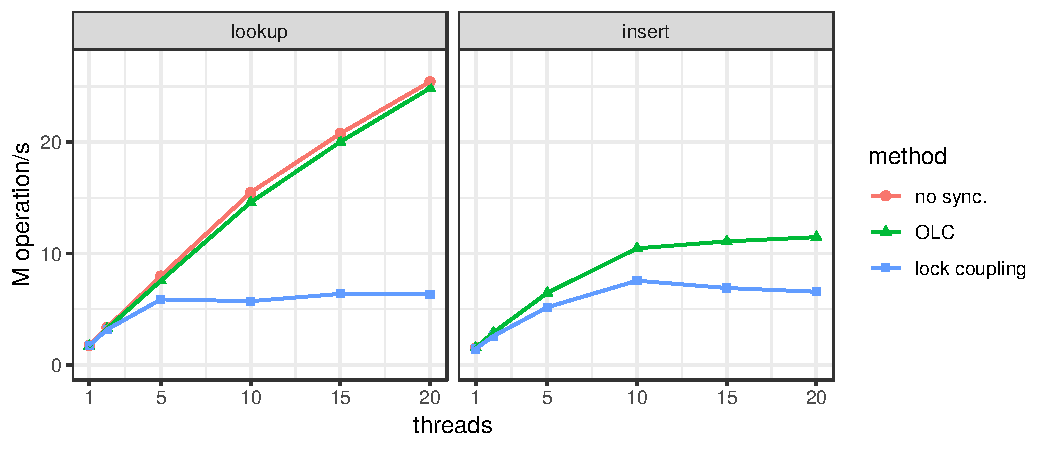
\includegraphics[width=\linewidth]{scale.pdf}
  \vspace{0.2cm}
  \caption{Scalability on 10-core system for B-tree operations (100M values).}
  \label{fig:scale}
\end{figure}

As Figure~\ref{fig:scale} shows, the results change dramatically once we use multiple threads.
For lookup, the scalability of OLC is near-linear up to 20 threads, even though the system has only 10 ``real cores''.
The OLC scalability for insert is also respectable (though not quite as linear because multi-threaded insertion approaches the memory bandwidth of our processor).
The figure also shows that the results of traditional lock coupling with read/write locks are significantly worse than OLC.
With 20 threads, lookup with OLC is 3.9$\times$ faster than traditional lock coupling.

\section{Summary}\label{sec:conc}

Optimistic Lock Coupling (OLC) is an effective synchronization method that combines the simplicity of traditional lock coupling with the superior scalability of lock-free approaches.
OLC is widely applicable and has already been successfully used to synchronize several data structures, including B-trees, binary search trees, and different trie variants.
These features make it highly attractive for modern database systems as well as performance-critical systems software in general.

\begin{thebibliography}{10}

\bibitem{DBLP:conf/spaa/BalmauGHZ16}
O.~Balmau, R.~Guerraoui, M.~Herlihy, and I.~Zablotchi.
\newblock Fast and robust memory reclamation for concurrent data structures.
\newblock In {\em SPAA}, 2016.

\bibitem{DBLP:journals/acta/BayerS77}
R.~Bayer and M.~Schkolnick.
\newblock Concurrency of operations on {B}-trees.
\newblock {\em Acta Informatica}, 9, 1977.

\bibitem{hot}
R.~Binna, E.~Zangerle, M.~Pichl, G.~Specht, and V.~Leis.
\newblock {HOT}: A height optimized trie index for main-memory database
  systems.
\newblock In {\em SIGMOD}, 2018.

\bibitem{DBLP:conf/ppopp/BronsonCCO10}
N.~G. Bronson, J.~Casper, H.~Chafi, and K.~Olukotun.
\newblock A practical concurrent binary search tree.
\newblock In {\em PPOPP}, 2010.

\bibitem{DBLP:conf/vldb/ChaHKK01}
S.~K. Cha, S.~Hwang, K.~Kim, and K.~Kwon.
\newblock Cache-conscious concurrency control of main-memory indexes on
  shared-memory multiprocessor systems.
\newblock In {\em VLDB}, 2001.

\bibitem{intel}
I.~Cutress.
\newblock {Intel} goes for 48-cores: {Cascade-AP} with multi-chip package
  coming soon.
\newblock
  \url{https://www.anandtech.com/show/13535/intel-goes-for-48cores-cascade-ap},
  2018 (accessed January, 2019).

\bibitem{DBLP:conf/cidr/FaleiroA17}
J.~M. Faleiro and D.~J. Abadi.
\newblock Latch-free synchronization in database systems: Silver bullet or
  fool's gold?
\newblock In {\em CIDR}, 2017.

\bibitem{DBLP:journals/ftdb/Graefe11}
G.~Graefe.
\newblock Modern {B}-tree techniques.
\newblock {\em Foundations and Trends in Databases}, 3(4), 2011.

\bibitem{DBLP:conf/hpca/KarnagelDRLLSL14}
T.~Karnagel, R.~Dementiev, R.~Rajwar, K.~Lai, T.~Legler, B.~Schlegel, and
  W.~Lehner.
\newblock Improving in-memory database index performance with
  {Intel}\({}^{\mbox{{\textregistered}}}\) transactional synchronization
  extensions.
\newblock In {\em HPCA}, 2014.

\bibitem{DBLP:journals/tods/LehmanY81}
P.~L. Lehman and S.~B. Yao.
\newblock Efficient locking for concurrent operations on {B}-trees.
\newblock {\em {ACM} Trans. Database Syst.}, 6(4), 1981.

\bibitem{leanstore}
V.~Leis, M.~Haubenschild, A.~Kemper, and T.~Neumann.
\newblock Leanstore: In-memory data management beyond main memory.
\newblock In {\em ICDE}, 2018.

\bibitem{art}
V.~Leis, A.~Kemper, and T.~Neumann.
\newblock The adaptive radix tree: {ARTful} indexing for main-memory databases.
\newblock In {\em ICDE}, 2013.

\bibitem{htmtkde}
V.~Leis, A.~Kemper, and T.~Neumann.
\newblock Scaling {HTM}-supported database transactions to many cores.
\newblock {\em {IEEE} Trans. Knowl. Data Eng.}, 28(2), 2016.

\bibitem{artsync}
V.~Leis, F.~Scheibner, A.~Kemper, and T.~Neumann.
\newblock The {ART} of practical synchronization.
\newblock In {\em DaMoN}, 2016.

\bibitem{DBLP:conf/icde/LevandoskiLS13a}
J.~J. Levandoski, D.~B. Lomet, and S.~Sengupta.
\newblock The {Bw}-tree: A {B}-tree for new hardware platforms.
\newblock In {\em ICDE}, 2013.

\bibitem{DBLP:journals/pvldb/MakreshanskiLS15}
D.~Makreshanski, J.~J. Levandoski, and R.~Stutsman.
\newblock To lock, swap, or elide: On the interplay of hardware transactional
  memory and lock-free indexing.
\newblock {\em {PVLDB}}, 8(11), 2015.

\bibitem{DBLP:dblp_conf/eurosys/MaoKM12}
Y.~Mao, E.~Kohler, and R.~T. Morris.
\newblock Cache craftiness for fast multicore key-value storage.
\newblock In {\em EuroSys}, 2012.

\bibitem{DBLP:journals/tpds/Michael04}
M.~M. Michael.
\newblock Hazard pointers: Safe memory reclamation for lock-free objects.
\newblock {\em {IEEE} Trans. Parallel Distrib. Syst.}, 15(6), 2004.

\bibitem{DBLP:journals/jacm/ShalevS06}
O.~Shalev and N.~Shavit.
\newblock Split-ordered lists: Lock-free extensible hash tables.
\newblock {\em J. {ACM}}, 53(3), 2006.

\bibitem{amd}
A.~Shilov.
\newblock {AMD} previews {EPYC} ‘{Rome}’ processor: Up to 64 {Zen} 2 cores.
\newblock
  \url{https://www.anandtech.com/show/13561/amd-previews-epyc-rome-processor-up-to-64-zen-2-cores},
  2018 (accessed January, 2019).

\bibitem{DBLP:conf/sosp/TuZKLM13}
S.~Tu, W.~Zheng, E.~Kohler, B.~Liskov, and S.~Madden.
\newblock Speedy transactions in multicore in-memory databases.
\newblock In {\em SOSP}, 2013.

\bibitem{buzzword}
Z.~Wang, A.~Pavlo, H.~Lim, V.~Leis, H.~Zhang, M.~Kaminsky, and D.~Andersen.
\newblock Building a {Bw}-tree takes more than just buzz words.
\newblock In {\em SIGMOD}, 2018.

\end{thebibliography}


%\bibliographystyle{abbrv}
%\bibliography{main}

\end{document}

\end{article}
\begin{article}
	{Human-in-the-loop Artificial Intelligence for Fighting Online Misinformation: Challenges and Opportunities}
	{Gianluca Demartini}
	\pdfminorversion=5
\documentclass[11pt]{article}
\usepackage{deauthor,times,graphicx,caption,microtype}
\usepackage{hyperref}
\usepackage{listings}
\usepackage{booktabs}

\begin{document}

\title{Optimistic Lock Coupling: A Scalable and Efficient General-Purpose Synchronization Method}

\author{Viktor Leis, Michael Haubenschild\raisebox{0.9ex}{$\ast$}, Thomas Neumann\\ Technische Universit{\"a}t M{\"u}nchen \hspace{0.7cm} Tableau Software\raisebox{0.9ex}{$\ast$} \\ {\{leis,neumann\}{@}in.tum.de} \hspace{0.7cm} {mhaubenschild{@}tableau.com\raisebox{0.9ex}{$\ast$}}}

\maketitle

\begin{abstract}
As the number of cores on commodity processors continues to increase, scalability becomes more and more crucial for overall performance.
Scalable and efficient concurrent data structures are particularly important, as these are often the building blocks of parallel algorithms.
Unfortunately, traditional synchronization techniques based on fine-grained locking have been shown to be unscalable on modern multi-core CPUs.
Lock-free data structures, on the other hand, are extremely difficult to design and often incur significant overhead.

In this work, we make the case for Optimistic Lock Coupling as a practical alternative to both traditional locking and the lock-free approach.
We show that Optimistic Lock Coupling is highly scalable and almost as simple to implement as traditional lock coupling.
Another important advantage is that it is easily applicable to most tree-like data structures.
We therefore argue that Optimistic Lock Coupling, rather than a complex and error-prone custom synchronization protocol, should be the default choice for performance-critical data structures.
\end{abstract}

\section{Introduction}

% more and more cores
Today, Intel's commodity server processors have up to 28 cores and its upcoming microarchitecture will have up to 48 cores per socket~\cite{intel}.
Similarly, AMD currently stands at 32 cores and this number is expected to double in the next generation~\cite{amd}.
Since both platforms support simultaneous multithreading (also known as hyperthreading), affordable commodity servers (with up to two sockets) will soon routinely have between 100 and 200 hardware threads.

% data structure scalability is important
With such a high degree of hardware parallelism, efficient data processing crucially depends on how well concurrent data structures scale.
Internally, database systems use a plethora of data structures like table heaps, internal work queues, and, most importantly, index structures.
Any of these can easily become a scalability (and therefore overall performance) bottleneck on many-core CPUs.

% traditional synchronization: fine-grained locks, slow, cache invalidation
Traditionally, database systems synchronize internal data structures using fine-grained reader/writer locks\footnote{In this work, we focus on data structure synchronization rather than high-level transaction semantics and therefore use the term {\em lock} for what would typically be called {\em latch} in the database literature. We thus follow common computer science (rather than database) terminology.}.
Unfortunately, while fine-grained locking makes lock contention unlikely, it still results in bad scalability because lock acquisition and release require writing to shared memory.
Due to the way cache coherency is implemented on modern multi-core CPUs, these writes cause additional cache misses\footnote{The cache coherency protocol ensures that all copies of a cache line on other cores are invalidated before the write can proceed.} and the cache line containing the lock's internal data becomes a point of physical contention.
As a result, any frequently-accessed lock (e.g., the lock of the root node of a B-tree) severely limits scalability.

% lock-free bw-tree: no more latches, but indirections, extremely complex
Lock-free data structures like the Bw-tree~\cite{DBLP:conf/icde/LevandoskiLS13a} (a lock-free B-tree variant) or the Split-Ordered List~\cite{DBLP:journals/jacm/ShalevS06} (a lock-free hash table) do not acquire any locks and therefore generally scale much better than locking-based approaches (in particular for read-mostly workloads).
However, lock-free synchronization has other downsides:
First, it is very difficult and results in extremely complex and error-prone code (when compared to locking).
Second, because the functionality of atomic primitives provided by the hardware (e.g., atomically compare-and-swap 8 bytes) is limited, complex operations require additional indirections within the data structure.
For example, the Bw-tree requires an indirection table and the Split-Ordered List requires ``dummy nodes'', resulting in overhead due to additional cache misses.

% OLC for the win
In this paper we make the case for {\em Optimistic Lock Coupling (OLC)}, a synchronization method that combines some of the best properties of lock-based and lock-free synchronization.
OLC utilizes a special lock type that can be used in two modes:
The first mode is similar to a traditional mutex and excludes other threads by physically acquiring the underlying lock.
In the second mode, reads can proceed optimistically by validating a version counter that is embedded in the lock (similar to optimistic concurrency control).
The first mode is typically used by writers and the second mode by readers.
Besides this special lock type, OLC is based on the observation that optimistic lock validations can be interleaved/coupled---similar to the pair-wise interleaved lock acquisition of traditional lock coupling.
Hence, the name Optimistic Lock Coupling.

OLC has a number of desirable features:
\begin{itemize}
\item By reducing the number of writes to shared memory locations and thereby avoiding cache invalidations, it {\bf scales well} for most workloads.
\item In comparison to unsynchronized code, it requires few additional CPU instructions making it {\bf efficient}.
\item OLC is {\bf widely applicable} to different data structures. It has already been successfully used for synchronizing binary search trees~\cite{DBLP:conf/ppopp/BronsonCCO10}, tries~\cite{artsync}, trie/B-tree hybrids~\cite{DBLP:dblp_conf/eurosys/MaoKM12}, and B-trees~\cite{buzzword}.
\item In comparison to the lock-free paradigm, it is also {\bf easy to use} and requires few modifications to existing, single-threaded data structures.
\end{itemize}
Despite these positive features and its simplicity, OLC is not yet widely known.
The goal of this paper is therefore to popularize this simple idea and to make a case for it.
We argue that OLC deserves to be widely known.
It is a good default synchronization paradigm---more complex, data structure-specific protocols are seldom beneficial.

The rest of the paper is organized as follows.
Section~\ref{sec:related} discusses related work, tracing the history of OLC and its underlying ideas in the literature.
The core of the paper is Section~\ref{sec:olc}, which describes the ideas behind OLC and how it can be used to synchronize complex data structures.
In Section~\ref{sec:evaluation} we experimentally show that OLC has low overhead and scales well when used to synchronize an in-memory B-tree.
We summarize the paper in Section~\ref{sec:conc}.

\newpage
\section{Related Work}\label{sec:related}

Lock coupling has been proposed as a method for allowing concurrent operations on B-trees in 1977~\cite{DBLP:journals/acta/BayerS77}.
This traditional and still widely-used method, described in detail in Graefe's B-tree survey~\cite{DBLP:journals/ftdb/Graefe11}, is also called ``latch coupling'', ``hand-over-hand locking'', and ``crabbing''.
Because at most two locks are held at-a-time during tree traversal, this technique seemingly allows for a high degree of parallelism---in particular if read/write locks are used to enable inner nodes to be locked in shared mode.
However, as we show in Section~\ref{sec:evaluation}, on modern hardware lock acquisition (even in shared mode) results in suboptimal scalability.

An early alternative from 1981 is a B-tree variant called B-link tree~\cite{DBLP:journals/tods/LehmanY81}, which only holds a single lock at a time.
It is based on the observation that between the release of the parent lock and the acquisition of the child lock, the only ``dangerous'' thing that could have happened is the split of a child node (assuming one does not implement merge operations).
Thus, when a split happens, the key being searched might end up on a neighboring node to the right of the current child node.
A B-link tree traversal therefore detects this condition and, if needed, transparently proceeds to the neighboring node.
Releasing the parent lock early is highly beneficial when the child node needs to be fetched from disk.
For in-memory workloads, however, the B-link tree has the same scalability issues as lock coupling (it acquires just as many locks).

The next major advance, Optimistic Latch-Free Index Traversal (OLFIT)~\cite{DBLP:conf/vldb/ChaHKK01}, was proposed in 2001.
OLFIT introduced the idea of a combined lock/update counter, which we call {\em optimistic lock}. % , for lack of a better name,
Based on these per-node optimistic locks and the synchronization protocol of the B-link tree, OLFIT finally achieves good scalability on parallel processors.
The OLFIT protocol is fairly complex, as it requires both the non-trivial B-link protocol and optimistic locks.
Furthermore, like the B-link tree protocol, it does not support merging nodes, and is specific to B-trees (cannot easily be applied to other data structures).

In the following two decades, the growth of main-memory capacity led to much research into other data structures besides the venerable B-tree.
Particularly relevant for our discussion is Bronson et al.'s~\cite{DBLP:conf/ppopp/BronsonCCO10} concurrent binary search tree, which is based on optimistic version validation and has a sophisticated, data structure-specific synchronization protocol.
To the best of our knowledge, this 2010 paper is the first that, as part of its protocol, interleaves version validation across nodes---rather than validating each node separately like OLFIT.
In that paper, this idea is called ``hand-over-hand, optimistic validation'', while we prefer the term Optimistic Lock Coupling to highlight the close resemblance to traditional lock coupling.
Similarly, Mao et al.'s~\cite{DBLP:dblp_conf/eurosys/MaoKM12} Masstree (a concurrent hybrid trie/B-tree) is also based on the same ideas, but again uses them as part of a more complex protocol.

The Adaptive Radix Tree (ART)~\cite{art} is another recent in-memory data structure, which we proposed in 2013.
In contrast to the two data structures just mentioned, it was originally designed with single-threaded performance in mind without supporting concurrency.
To add support for concurrency, we initially started designing a custom protocol called Read-Optimized Write Exclusion (ROWEX)~\cite{artsync}, which turned out to be non-trivial and requires modifications of the underlying data structure\footnote{Note that ROWEX is already easier to apply to existing data structures than the lock-free approach. The difficulty depends on the data structure. Applying ROWEX is hard for B-trees with sorted keys and fairly easy for copy-on-write data structures like the Height Optimized Trie~\cite{hot}---with ART being somewhere in the middle.}.
However, fairly late in the project, we also realized, that OLC {\em alone} (rather than as part of a more complex protocol) is sufficient to synchronize ART.
No other changes to the data structure were necessary.
Both approaches were published and experimentally evaluated in a followup paper~\cite{artsync}, which shows that, despite its simplicity, OLC is efficient, scalable, and generally outperforms ROWEX.

Similar results were recently published regarding B-trees~\cite{buzzword}.
In this experimental study a simple OLC-based synchronization outperformed the Bw-tree~\cite{DBLP:conf/icde/LevandoskiLS13a}, a complex lock-free synchronization approach.
Another recent paper shows that for write-intensive workloads, locking often performs better than lock-free synchronization~\cite{DBLP:conf/cidr/FaleiroA17}.
These experiences indicate that OLC is a general-purpose synchronization paradigm and motivate the current paper.

%foster b-tree\cite{DBLP:journals/tods/GraefeKK12}
%Shasha theory~\cite{DBLP:journals/tods/ShashaG88}

\section{Optimistic Lock Coupling}\label{sec:olc}

% locks suck
The standard technique for inter-thread synchronization is mutual exclusion using fine-grained locks.
In a B-tree, for example, every node usually has its own associated lock, which is acquired before accessing that node.
The problem of locking on modern multi- and many-core processors is that lock acquisition and release require writing to the shared memory location that implements the lock.
This write causes exclusive ownership of the underlying cache line and invalidates copies of it on all other processor cores.
For hierarchical, tree-like data structures, the lock of the root node becomes a point of physical contention---even in read-only workloads and even when read/write locks are used.
Depending on the specific data structure, number of cores, cache coherency protocol implementation, cache topology, whether Non-Uniform Memory Access (NUMA) is used, locking can even result in multi-threaded performance that is worse than single-threaded execution.

% in b-trees this happens very much
The inherent pessimism of locking is particularly unfortunate for B-trees:
Despite the fact that logical modifications of the root node are very infrequent, every B-tree operation must lock the root node during tree traversal\footnote{To a lesser extent this obviously applies to all inner nodes, not just the root.}.
Even the vast majority of update operations (with the exception of splits and merges), only modify a single leaf node.
These observations indicate that a more optimistic approach, which does not require locking inner nodes, would be very beneficial for B-trees.

\subsection{Optimistic Locks}

% optimism to the rescue
As the name indicates, optimistic locks try to solve the scalability issues of traditional locks using an optimistic approach.
Instead of always physically acquiring locks, even for nodes that are unlikely to be modified simultaneously, after-the-fact validation is used to detect conflicts.
This is done by augmenting each lock with a version/update counter that is incremented on every modification.
Using this version counter, readers can optimistically proceed before validating that the version did not change to ensure that the read was safe.
If validation fails, the operation is restarted.

% details on opt locks
Using optimistic locks, a read-only node access (i.e., the majority of all operations in a B-tree) does not acquire the lock and does not increment the version counter.
Instead, it performs the following steps:
\begin{enumerate}
\item read lock version (restart if lock is not free)
\item access node
\item read the version again and validate that it has not changed in the meantime
\end{enumerate}
If the last step (the validation) fails, the operation has to be restarted.
Write operations, on the other hand, are more similar to traditional locking:
\begin{enumerate}
\item acquire lock (wait if necessary)
\item access/write to node
\item increment version and unlock node
\end{enumerate}
Writes can therefore protect a node from other writes.

% similar to locks
As we observed in an earlier paper~\cite{artsync}, because of similar semantics, optimistic locks can be hidden behind an API very similar to traditional read/write locks.
Both approaches have an exclusive lock mode, and acquiring a traditional lock in shared mode is analogous to optimistic version validation.
Furthermore, like with some implementations of traditional read/write locks, optimistic locks allow upgrading a shared lock to an exclusive lock.
Lock upgrades are, for example, used to avoid most B-tree update operations from having to lock inner nodes.
In our experience, the close resemblance of optimistic and traditional locks simplifies the reasoning about optimistic locks;
one can apply similar thinking as in traditional lock-based protocols.

\subsection{Lock Coupling with Optimistic Locks}

\begin{figure}
  \centering
  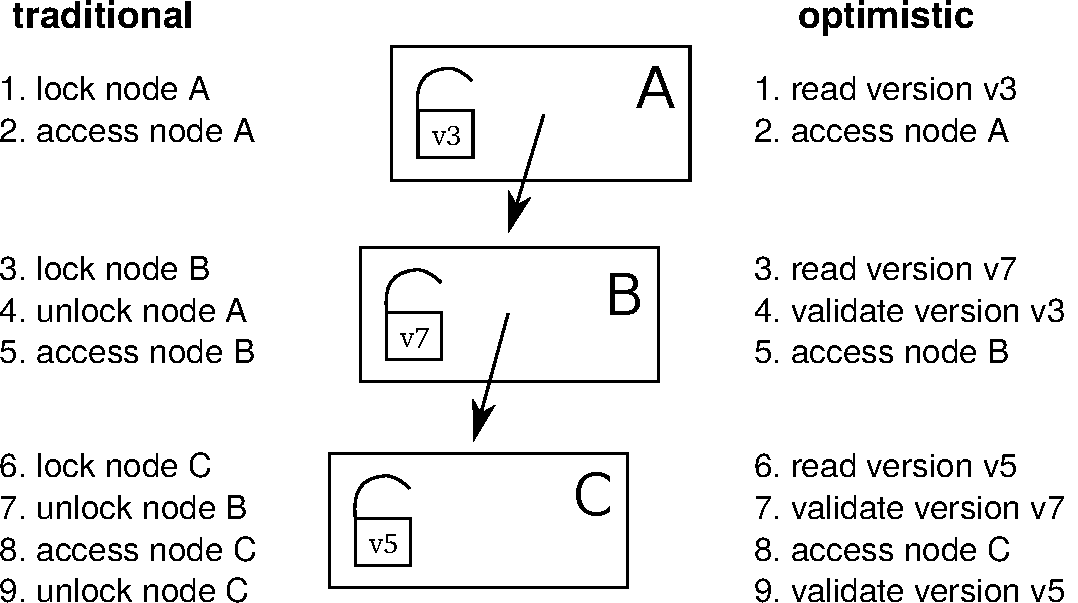
\includegraphics[width=0.65\linewidth]{olcall.pdf}
  \vspace{0.2cm}
  \caption{Comparison of a lookup operation in a 3-level tree using traditional lock coupling (left-hand side) vs.~optimistic lock coupling (right-hand side).}
  \label{fig:olc}
\end{figure}

The traditional and most common lock-based synchronization protocol for B-trees is lock coupling, which interleaves lock acquisitions while holding at most two locks at a time.
If, as we observed earlier, optimistic locks have similar semantics as traditional locks, it is natural to ask whether lock coupling can be combined with optimistic locks.
And indeed the answer is yes: One can almost mechanically translate traditional lock coupling code to optimistic lock coupling code.
This is illustrated in Figure~\ref{fig:olc}, which compares the traversal in a tree of height 3 using traditional and optimistic locks.
As the figure shows, the main difference is that locking is translated to reading the version and that unlocking becomes validation of the previously read version.
This simple change provides efficient lock-free tree traversal without the need to design a complex synchronization protocol.

It is important to emphasize the conceptual simplicity of OLC in comparison to data structures that use custom protocols like the Bw-tree~\cite{DBLP:conf/icde/LevandoskiLS13a}.
To implement lock-free access, the Bw-tree requires an indirection table, delta nodes, complex splitting and merging logic, retry logic, etc.
OLC, on the other hand, can directly be applied to B-trees mostly by adding the appropriate optimistic locking code and without modifying the node layout itself.
Therefore, OpenBw-Tree, an open source implementation of the Bw-tree, requires an order of magnitude more code than a B-tree based on OLC\footnote{Both implementations are available on GitHub: \url{https://github.com/wangziqi2016/index-microbench}}.
Given how difficult it is to develop, validate, and debug lock-free code, simplicity is obviously a major advantage.

\subsection{Correctness Aspects}

\begin{figure}
  % \centering
  %[basicstyle=\normalsize\ttfamily,showstringspaces=false,columns=fullflexible,breaklines=false,breakatwhitespace=true,numbers=none,numberstyle=\small,style=C,keepspaces=true]
\begin{lstlisting}[basicstyle=\ttfamily,language=C++,numbers=left,numberstyle=\small]
std::atomic<BTreeNode*> root;

// search for key in B+tree, returns payload in resultOut
bool lookup(Key key, Value& resultOut) {
   BTreeNode* node = root.load();
   uint64_t nodeVersion = node->readLockOrRestart();
   if (node != root.load()) // make sure the root is still the root
      restart();

   BTreeInner<Key>* parent = nullptr;
   uint64_t parentVersion = 0;

   while (node->isInner()) {
      auto inner = (BTreeInner*)node;

      // unlock parent and make current node the parent
      if (parent)
         parent->readUnlockOrRestart(parentVersion);
      parent = inner;
      parentVersion = nodeVersion;

      // search for next node
      node = inner->findChild(key);
      // validate 'inner' to ensure that 'node' pointer is valid
      inner->checkOrRestart(nodeVersion);
      // now it safe to dereference 'node' pointer (read its version)
      nodeVersion = node->readLockOrRestart();
   }

   // search in leaf and retrieve payload
   auto leaf = (BTreeLeaf*)node;
   bool success = leaf->findValue(key, resultOut);

   // unlock everything
   if (parent)
      parent->readUnlockOrRestart(parentVersion);
   node->readUnlockOrRestart(nodeVersion);

   return success;
}
\end{lstlisting}
  \vspace{0.2cm}
  \caption{B-tree lookup code using OLC. For simplicity, the restart logic is not shown.}
  \label{fig:lookup}
\end{figure}

So far, we have introduced the high-level ideas behind OLC and have stressed its similarity to traditional lock coupling.
Let us now discuss some cases where the close similarity between lock coupling and OLC breaks down.
To make this more concrete, we show the B-tree lookup code in Figure~\ref{fig:lookup}.
In the code, \texttt{readLockOrRestart} reads the lock version and \texttt{readUnlockOrRestart} validates that the read was correct.

One issue with OLC is that any pointer speculatively read from a node may point to invalid memory (if that node is modified concurrently).
Dereferencing such a pointer (e.g., to read its optimistic lock), may cause a segmentation fault or undefined behavior.
In the code shown in Figure~\ref{fig:lookup}, this problem is prevented by the extra check in line 25, which ensures that the read from the node containing the pointer was correct.
Without this additional validation, the code would in line 27 dereference the pointer speculatively read in line 23.
Note that the implementation of \texttt{checkOrRestart} is actually identical to \texttt{readUnlockOrRestart}.
We chose to give it a different name to highlight the fact that this extra check would not be necessary with read/write locks.

Another potential issue with optimistic locks is code that does not terminate.
Code that speculatively accesses a node, like an intra-node binary search, should be written in a way such that it always terminates---even in the presence of concurrent writes.
Otherwise, the validation code that detects the concurrent write will never run.
The binary search of a B-tree, for example, needs to be written in such a way that each comparison makes progress.
For some data structures that do not require loops in the traversal code (like ART) termination is trivially true.

\subsection{Implementation Details}

% implementation, efficiency
To implement an optimistic lock, one can combine the lock and the version counter into a single 64-bit\footnote{Even after subtracting one bit for the lock status, a back-of-the-envelope calculation can show that 63 bits are large enough to never overflow in practice.} word~\cite{artsync}.
A typical read operation will therefore merely consist of reading this version counter atomically.
In C++11 this can be implemented using the \texttt{std::atomic} type.

On x86, atomic reads are cheap because of x86's strong memory order guarantees.
No memory fences are required for sequentially-consistent loads, which are translated (by both GCC and clang) into standard \texttt{MOV} instructions.
Hence, the only effect of \texttt{std::atomic} for loads is preventing instruction re-ordering.
This makes version access and validation cheap.
Acquiring and releasing an optimistic lock in exclusive mode has comparable cost to a traditional lock:
A fairly expensive sequentially-consistent store is needed for acquiring a lock, while a standard \texttt{MOV} suffices for releasing it.
A simple sinlock-based implementation of optimistic locks can be found in the appendix of an earlier paper~\cite{artsync}.

OLC code must be able to handle restarts since validation or lock upgrade can fail due to concurrent writers.
Restarts can easily be implemented by wrapping the data structure operation in a loop (for simplicity not shown in Figure~\ref{fig:lookup}).
Such a loop also enables limiting the number of optimistic retry operations and falling back to pessimistic locking in cases of very heavy contention.
The ability to fall back to traditional locking is a major advantage of OLC in terms of robustness over lock-free approaches, which do not have this option.

In addition to the optimistic shared mode and the exclusive mode, optimistic locks also support a ``shared pessimistic'' mode, which physically acquires the lock in shared mode (allowing multiple concurrent readers but no writers).
This mode is useful for table (or range) scans that touch many tuples on a leaf page (which would otherwise easily abort).
Finally, let us mention that large range scans and table scans, should be broken up into several per-node traversals as is done in the LeanStore~\cite{leanstore} system.

Like all lock-free data structures, but unlike traditional locking and Hardware Transactional Memory~\cite{DBLP:conf/hpca/KarnagelDRLLSL14,DBLP:journals/pvldb/MakreshanskiLS15,htmtkde}, OLC requires care when deleting (and reusing) nodes.
The reason is that a deleting thread can never be sure that a node can be reclaimed because other threads might still be optimistically reading from that node.
Therefore, standard solutions like epoch-based reclamation~\cite{DBLP:conf/sosp/TuZKLM13}, hazard pointers~\cite{DBLP:journals/tpds/Michael04}, or optimized hazard pointers~\cite{DBLP:conf/spaa/BalmauGHZ16} need to be used.
These memory reclamation techniques are, however, largely orthogonal to the synchronization protocol itself.

%-lock-free is not a strong guarantee

\newpage
\section{Evaluation}\label{sec:evaluation}

Let us now experimentally evaluate the overhead and scalability of OLC.
For the experiments, we use an in-memory B+tree implemented in C++11 using templates, which is configured to use nodes of 4096 bytes, random 8 byte keys, and 8 byte payloads.
Based on this B-tree, we compare the following synchronization approaches:
\begin{itemize}
\item an OLC implementation\footnote{An almost identical OLC implementation is available on github: \url{https://github.com/wangziqi2016/index-microbench/tree/master/BTreeOLC}}
\item a variant based on traditional lock coupling and read/write locks
\item the unsynchronized B-tree, which obviously is only correct for read-only workloads but allows measuring the overhead of synchronization
\end{itemize}
Note that earlier work has compared the OLC implementation with a Bw-tree implementation~\cite{buzzword} and other state-of-the-art in-memory index structures.

We use a Haswell EP system with an Intel Xeon E5-2687W v3 CPU, which has 10 cores (20 ``Hyper-Threads'') and 25~MB of L3 cache.
The system is running Ubuntu 18.10 and we use GCC 8.2.0 to compile our code.
The CPU counters are obtained using the Linux perf API\footnote{We use the following convenience wrapper: \url{https://github.com/viktorleis/perfevent}}.

\begin{table}
  \caption{Performance and CPU counters for lookup and insert operations in a B-tree with 100M keys. We perform 100M operations and normalize the CPU counters by that number.}
  \label{tab:overhead}
  \centering
  \begin{tabular}{lrrrrrrr}\toprule
                    &         &        &        & instruc-  & L1     & L3     & branch \\
                    & threads & M op/s & cycles & tions & misses & misses & misses \\\midrule
lookup (no sync.)   & 1       & 1.72   & 2028   & 283     & 39.1   & 14.9   & 16.1   \\
lookup (OLC)        & 1       & 1.65   & 2107   & 370     & 43.9   & 15.1   & 16.7   \\
lookup (lock coup.) & 1       & 1.72   & 2078   & 365     & 42.3   & 16.9   & 15.7   \\\midrule
insert (no sync.)   & 1       & 1.51   & 2286   & 530     & 59.8   & 31.1   & 17.3   \\
insert (OLC)        & 1       & 1.50   & 2303   & 629     & 61.2   & 31.1   & 16.5   \\
insert (lock coup.) & 1       & 1.41   & 2473   & 644     & 61.0   & 31.0   & 17.2   \\\midrule
lookup (no sync.)   & 10      & 15.48  & 2058   & 283     & 38.6   & 15.5   & 16.0   \\
lookup (OLC)        & 10      & 14.60  & 2187   & 370     & 43.8   & 15.8   & 16.8   \\
lookup (lock coup.) & 10      & 5.71   & 5591   & 379     & 54.2   & 17.0   & 14.8   \\\midrule
insert (no sync.)   & 10      & -      & -      & -       & -      & -      & -      \\
insert (OLC)        & 10      & 10.46  & 2940   & 656     & 62.0   & 32.5   & 16.8   \\
insert (lock coup.) & 10      & 7.55   & 4161   & 667     & 75.0   & 28.6   & 16.2   \\
    \bottomrule
\end{tabular}
\end{table}

Table~\ref{tab:overhead} compares the performance and CPU counters for lookup and insert operations in a B-tree with 100M keys.
With {\em single-threaded} execution, we observe that all three approaches have very similar performance.
Adding traditional or optimistic locks to unsynchronized B-tree code results in up to 30\% of additional instructions without affecting single-threaded performance much.

\begin{figure}
  \centering
  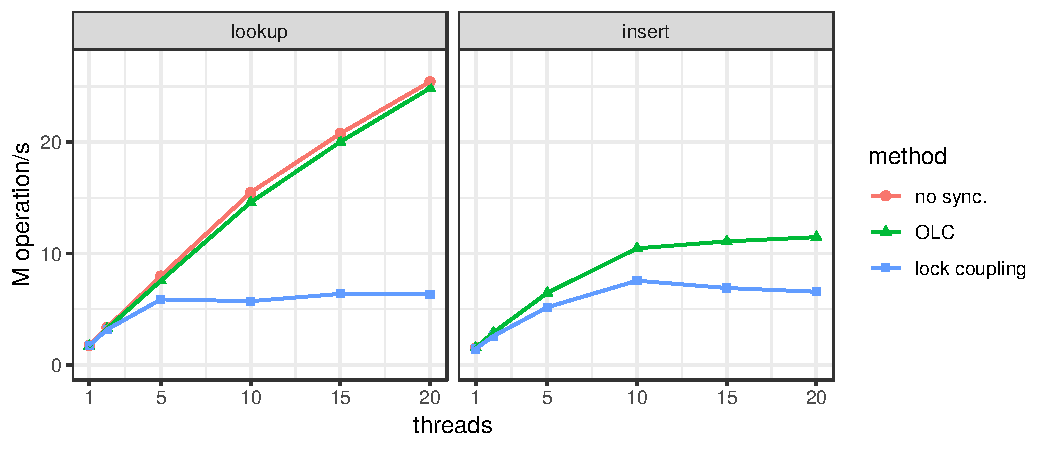
\includegraphics[width=\linewidth]{scale.pdf}
  \vspace{0.2cm}
  \caption{Scalability on 10-core system for B-tree operations (100M values).}
  \label{fig:scale}
\end{figure}

As Figure~\ref{fig:scale} shows, the results change dramatically once we use multiple threads.
For lookup, the scalability of OLC is near-linear up to 20 threads, even though the system has only 10 ``real cores''.
The OLC scalability for insert is also respectable (though not quite as linear because multi-threaded insertion approaches the memory bandwidth of our processor).
The figure also shows that the results of traditional lock coupling with read/write locks are significantly worse than OLC.
With 20 threads, lookup with OLC is 3.9$\times$ faster than traditional lock coupling.

\section{Summary}\label{sec:conc}

Optimistic Lock Coupling (OLC) is an effective synchronization method that combines the simplicity of traditional lock coupling with the superior scalability of lock-free approaches.
OLC is widely applicable and has already been successfully used to synchronize several data structures, including B-trees, binary search trees, and different trie variants.
These features make it highly attractive for modern database systems as well as performance-critical systems software in general.

\begin{thebibliography}{10}

\bibitem{DBLP:conf/spaa/BalmauGHZ16}
O.~Balmau, R.~Guerraoui, M.~Herlihy, and I.~Zablotchi.
\newblock Fast and robust memory reclamation for concurrent data structures.
\newblock In {\em SPAA}, 2016.

\bibitem{DBLP:journals/acta/BayerS77}
R.~Bayer and M.~Schkolnick.
\newblock Concurrency of operations on {B}-trees.
\newblock {\em Acta Informatica}, 9, 1977.

\bibitem{hot}
R.~Binna, E.~Zangerle, M.~Pichl, G.~Specht, and V.~Leis.
\newblock {HOT}: A height optimized trie index for main-memory database
  systems.
\newblock In {\em SIGMOD}, 2018.

\bibitem{DBLP:conf/ppopp/BronsonCCO10}
N.~G. Bronson, J.~Casper, H.~Chafi, and K.~Olukotun.
\newblock A practical concurrent binary search tree.
\newblock In {\em PPOPP}, 2010.

\bibitem{DBLP:conf/vldb/ChaHKK01}
S.~K. Cha, S.~Hwang, K.~Kim, and K.~Kwon.
\newblock Cache-conscious concurrency control of main-memory indexes on
  shared-memory multiprocessor systems.
\newblock In {\em VLDB}, 2001.

\bibitem{intel}
I.~Cutress.
\newblock {Intel} goes for 48-cores: {Cascade-AP} with multi-chip package
  coming soon.
\newblock
  \url{https://www.anandtech.com/show/13535/intel-goes-for-48cores-cascade-ap},
  2018 (accessed January, 2019).

\bibitem{DBLP:conf/cidr/FaleiroA17}
J.~M. Faleiro and D.~J. Abadi.
\newblock Latch-free synchronization in database systems: Silver bullet or
  fool's gold?
\newblock In {\em CIDR}, 2017.

\bibitem{DBLP:journals/ftdb/Graefe11}
G.~Graefe.
\newblock Modern {B}-tree techniques.
\newblock {\em Foundations and Trends in Databases}, 3(4), 2011.

\bibitem{DBLP:conf/hpca/KarnagelDRLLSL14}
T.~Karnagel, R.~Dementiev, R.~Rajwar, K.~Lai, T.~Legler, B.~Schlegel, and
  W.~Lehner.
\newblock Improving in-memory database index performance with
  {Intel}\({}^{\mbox{{\textregistered}}}\) transactional synchronization
  extensions.
\newblock In {\em HPCA}, 2014.

\bibitem{DBLP:journals/tods/LehmanY81}
P.~L. Lehman and S.~B. Yao.
\newblock Efficient locking for concurrent operations on {B}-trees.
\newblock {\em {ACM} Trans. Database Syst.}, 6(4), 1981.

\bibitem{leanstore}
V.~Leis, M.~Haubenschild, A.~Kemper, and T.~Neumann.
\newblock Leanstore: In-memory data management beyond main memory.
\newblock In {\em ICDE}, 2018.

\bibitem{art}
V.~Leis, A.~Kemper, and T.~Neumann.
\newblock The adaptive radix tree: {ARTful} indexing for main-memory databases.
\newblock In {\em ICDE}, 2013.

\bibitem{htmtkde}
V.~Leis, A.~Kemper, and T.~Neumann.
\newblock Scaling {HTM}-supported database transactions to many cores.
\newblock {\em {IEEE} Trans. Knowl. Data Eng.}, 28(2), 2016.

\bibitem{artsync}
V.~Leis, F.~Scheibner, A.~Kemper, and T.~Neumann.
\newblock The {ART} of practical synchronization.
\newblock In {\em DaMoN}, 2016.

\bibitem{DBLP:conf/icde/LevandoskiLS13a}
J.~J. Levandoski, D.~B. Lomet, and S.~Sengupta.
\newblock The {Bw}-tree: A {B}-tree for new hardware platforms.
\newblock In {\em ICDE}, 2013.

\bibitem{DBLP:journals/pvldb/MakreshanskiLS15}
D.~Makreshanski, J.~J. Levandoski, and R.~Stutsman.
\newblock To lock, swap, or elide: On the interplay of hardware transactional
  memory and lock-free indexing.
\newblock {\em {PVLDB}}, 8(11), 2015.

\bibitem{DBLP:dblp_conf/eurosys/MaoKM12}
Y.~Mao, E.~Kohler, and R.~T. Morris.
\newblock Cache craftiness for fast multicore key-value storage.
\newblock In {\em EuroSys}, 2012.

\bibitem{DBLP:journals/tpds/Michael04}
M.~M. Michael.
\newblock Hazard pointers: Safe memory reclamation for lock-free objects.
\newblock {\em {IEEE} Trans. Parallel Distrib. Syst.}, 15(6), 2004.

\bibitem{DBLP:journals/jacm/ShalevS06}
O.~Shalev and N.~Shavit.
\newblock Split-ordered lists: Lock-free extensible hash tables.
\newblock {\em J. {ACM}}, 53(3), 2006.

\bibitem{amd}
A.~Shilov.
\newblock {AMD} previews {EPYC} ‘{Rome}’ processor: Up to 64 {Zen} 2 cores.
\newblock
  \url{https://www.anandtech.com/show/13561/amd-previews-epyc-rome-processor-up-to-64-zen-2-cores},
  2018 (accessed January, 2019).

\bibitem{DBLP:conf/sosp/TuZKLM13}
S.~Tu, W.~Zheng, E.~Kohler, B.~Liskov, and S.~Madden.
\newblock Speedy transactions in multicore in-memory databases.
\newblock In {\em SOSP}, 2013.

\bibitem{buzzword}
Z.~Wang, A.~Pavlo, H.~Lim, V.~Leis, H.~Zhang, M.~Kaminsky, and D.~Andersen.
\newblock Building a {Bw}-tree takes more than just buzz words.
\newblock In {\em SIGMOD}, 2018.

\end{thebibliography}


%\bibliographystyle{abbrv}
%\bibliography{main}

\end{document}

\end{article}




\end{articlesection}

%\begin{articlesection}{Imagine All the People and AI in the Future of Work}
%\begin{article}
%{Capturing Human Factors to Optimize Crowdsourced Label
%Acquisition through Active Learning}
%{Senjuti Basu Roy}
%\pdfminorversion=5
\documentclass[11pt]{article}
\usepackage{deauthor,times,graphicx,caption,microtype}
\usepackage{hyperref}
\usepackage{listings}
\usepackage{booktabs}

\begin{document}

\title{Optimistic Lock Coupling: A Scalable and Efficient General-Purpose Synchronization Method}

\author{Viktor Leis, Michael Haubenschild\raisebox{0.9ex}{$\ast$}, Thomas Neumann\\ Technische Universit{\"a}t M{\"u}nchen \hspace{0.7cm} Tableau Software\raisebox{0.9ex}{$\ast$} \\ {\{leis,neumann\}{@}in.tum.de} \hspace{0.7cm} {mhaubenschild{@}tableau.com\raisebox{0.9ex}{$\ast$}}}

\maketitle

\begin{abstract}
As the number of cores on commodity processors continues to increase, scalability becomes more and more crucial for overall performance.
Scalable and efficient concurrent data structures are particularly important, as these are often the building blocks of parallel algorithms.
Unfortunately, traditional synchronization techniques based on fine-grained locking have been shown to be unscalable on modern multi-core CPUs.
Lock-free data structures, on the other hand, are extremely difficult to design and often incur significant overhead.

In this work, we make the case for Optimistic Lock Coupling as a practical alternative to both traditional locking and the lock-free approach.
We show that Optimistic Lock Coupling is highly scalable and almost as simple to implement as traditional lock coupling.
Another important advantage is that it is easily applicable to most tree-like data structures.
We therefore argue that Optimistic Lock Coupling, rather than a complex and error-prone custom synchronization protocol, should be the default choice for performance-critical data structures.
\end{abstract}

\section{Introduction}

% more and more cores
Today, Intel's commodity server processors have up to 28 cores and its upcoming microarchitecture will have up to 48 cores per socket~\cite{intel}.
Similarly, AMD currently stands at 32 cores and this number is expected to double in the next generation~\cite{amd}.
Since both platforms support simultaneous multithreading (also known as hyperthreading), affordable commodity servers (with up to two sockets) will soon routinely have between 100 and 200 hardware threads.

% data structure scalability is important
With such a high degree of hardware parallelism, efficient data processing crucially depends on how well concurrent data structures scale.
Internally, database systems use a plethora of data structures like table heaps, internal work queues, and, most importantly, index structures.
Any of these can easily become a scalability (and therefore overall performance) bottleneck on many-core CPUs.

% traditional synchronization: fine-grained locks, slow, cache invalidation
Traditionally, database systems synchronize internal data structures using fine-grained reader/writer locks\footnote{In this work, we focus on data structure synchronization rather than high-level transaction semantics and therefore use the term {\em lock} for what would typically be called {\em latch} in the database literature. We thus follow common computer science (rather than database) terminology.}.
Unfortunately, while fine-grained locking makes lock contention unlikely, it still results in bad scalability because lock acquisition and release require writing to shared memory.
Due to the way cache coherency is implemented on modern multi-core CPUs, these writes cause additional cache misses\footnote{The cache coherency protocol ensures that all copies of a cache line on other cores are invalidated before the write can proceed.} and the cache line containing the lock's internal data becomes a point of physical contention.
As a result, any frequently-accessed lock (e.g., the lock of the root node of a B-tree) severely limits scalability.

% lock-free bw-tree: no more latches, but indirections, extremely complex
Lock-free data structures like the Bw-tree~\cite{DBLP:conf/icde/LevandoskiLS13a} (a lock-free B-tree variant) or the Split-Ordered List~\cite{DBLP:journals/jacm/ShalevS06} (a lock-free hash table) do not acquire any locks and therefore generally scale much better than locking-based approaches (in particular for read-mostly workloads).
However, lock-free synchronization has other downsides:
First, it is very difficult and results in extremely complex and error-prone code (when compared to locking).
Second, because the functionality of atomic primitives provided by the hardware (e.g., atomically compare-and-swap 8 bytes) is limited, complex operations require additional indirections within the data structure.
For example, the Bw-tree requires an indirection table and the Split-Ordered List requires ``dummy nodes'', resulting in overhead due to additional cache misses.

% OLC for the win
In this paper we make the case for {\em Optimistic Lock Coupling (OLC)}, a synchronization method that combines some of the best properties of lock-based and lock-free synchronization.
OLC utilizes a special lock type that can be used in two modes:
The first mode is similar to a traditional mutex and excludes other threads by physically acquiring the underlying lock.
In the second mode, reads can proceed optimistically by validating a version counter that is embedded in the lock (similar to optimistic concurrency control).
The first mode is typically used by writers and the second mode by readers.
Besides this special lock type, OLC is based on the observation that optimistic lock validations can be interleaved/coupled---similar to the pair-wise interleaved lock acquisition of traditional lock coupling.
Hence, the name Optimistic Lock Coupling.

OLC has a number of desirable features:
\begin{itemize}
\item By reducing the number of writes to shared memory locations and thereby avoiding cache invalidations, it {\bf scales well} for most workloads.
\item In comparison to unsynchronized code, it requires few additional CPU instructions making it {\bf efficient}.
\item OLC is {\bf widely applicable} to different data structures. It has already been successfully used for synchronizing binary search trees~\cite{DBLP:conf/ppopp/BronsonCCO10}, tries~\cite{artsync}, trie/B-tree hybrids~\cite{DBLP:dblp_conf/eurosys/MaoKM12}, and B-trees~\cite{buzzword}.
\item In comparison to the lock-free paradigm, it is also {\bf easy to use} and requires few modifications to existing, single-threaded data structures.
\end{itemize}
Despite these positive features and its simplicity, OLC is not yet widely known.
The goal of this paper is therefore to popularize this simple idea and to make a case for it.
We argue that OLC deserves to be widely known.
It is a good default synchronization paradigm---more complex, data structure-specific protocols are seldom beneficial.

The rest of the paper is organized as follows.
Section~\ref{sec:related} discusses related work, tracing the history of OLC and its underlying ideas in the literature.
The core of the paper is Section~\ref{sec:olc}, which describes the ideas behind OLC and how it can be used to synchronize complex data structures.
In Section~\ref{sec:evaluation} we experimentally show that OLC has low overhead and scales well when used to synchronize an in-memory B-tree.
We summarize the paper in Section~\ref{sec:conc}.

\newpage
\section{Related Work}\label{sec:related}

Lock coupling has been proposed as a method for allowing concurrent operations on B-trees in 1977~\cite{DBLP:journals/acta/BayerS77}.
This traditional and still widely-used method, described in detail in Graefe's B-tree survey~\cite{DBLP:journals/ftdb/Graefe11}, is also called ``latch coupling'', ``hand-over-hand locking'', and ``crabbing''.
Because at most two locks are held at-a-time during tree traversal, this technique seemingly allows for a high degree of parallelism---in particular if read/write locks are used to enable inner nodes to be locked in shared mode.
However, as we show in Section~\ref{sec:evaluation}, on modern hardware lock acquisition (even in shared mode) results in suboptimal scalability.

An early alternative from 1981 is a B-tree variant called B-link tree~\cite{DBLP:journals/tods/LehmanY81}, which only holds a single lock at a time.
It is based on the observation that between the release of the parent lock and the acquisition of the child lock, the only ``dangerous'' thing that could have happened is the split of a child node (assuming one does not implement merge operations).
Thus, when a split happens, the key being searched might end up on a neighboring node to the right of the current child node.
A B-link tree traversal therefore detects this condition and, if needed, transparently proceeds to the neighboring node.
Releasing the parent lock early is highly beneficial when the child node needs to be fetched from disk.
For in-memory workloads, however, the B-link tree has the same scalability issues as lock coupling (it acquires just as many locks).

The next major advance, Optimistic Latch-Free Index Traversal (OLFIT)~\cite{DBLP:conf/vldb/ChaHKK01}, was proposed in 2001.
OLFIT introduced the idea of a combined lock/update counter, which we call {\em optimistic lock}. % , for lack of a better name,
Based on these per-node optimistic locks and the synchronization protocol of the B-link tree, OLFIT finally achieves good scalability on parallel processors.
The OLFIT protocol is fairly complex, as it requires both the non-trivial B-link protocol and optimistic locks.
Furthermore, like the B-link tree protocol, it does not support merging nodes, and is specific to B-trees (cannot easily be applied to other data structures).

In the following two decades, the growth of main-memory capacity led to much research into other data structures besides the venerable B-tree.
Particularly relevant for our discussion is Bronson et al.'s~\cite{DBLP:conf/ppopp/BronsonCCO10} concurrent binary search tree, which is based on optimistic version validation and has a sophisticated, data structure-specific synchronization protocol.
To the best of our knowledge, this 2010 paper is the first that, as part of its protocol, interleaves version validation across nodes---rather than validating each node separately like OLFIT.
In that paper, this idea is called ``hand-over-hand, optimistic validation'', while we prefer the term Optimistic Lock Coupling to highlight the close resemblance to traditional lock coupling.
Similarly, Mao et al.'s~\cite{DBLP:dblp_conf/eurosys/MaoKM12} Masstree (a concurrent hybrid trie/B-tree) is also based on the same ideas, but again uses them as part of a more complex protocol.

The Adaptive Radix Tree (ART)~\cite{art} is another recent in-memory data structure, which we proposed in 2013.
In contrast to the two data structures just mentioned, it was originally designed with single-threaded performance in mind without supporting concurrency.
To add support for concurrency, we initially started designing a custom protocol called Read-Optimized Write Exclusion (ROWEX)~\cite{artsync}, which turned out to be non-trivial and requires modifications of the underlying data structure\footnote{Note that ROWEX is already easier to apply to existing data structures than the lock-free approach. The difficulty depends on the data structure. Applying ROWEX is hard for B-trees with sorted keys and fairly easy for copy-on-write data structures like the Height Optimized Trie~\cite{hot}---with ART being somewhere in the middle.}.
However, fairly late in the project, we also realized, that OLC {\em alone} (rather than as part of a more complex protocol) is sufficient to synchronize ART.
No other changes to the data structure were necessary.
Both approaches were published and experimentally evaluated in a followup paper~\cite{artsync}, which shows that, despite its simplicity, OLC is efficient, scalable, and generally outperforms ROWEX.

Similar results were recently published regarding B-trees~\cite{buzzword}.
In this experimental study a simple OLC-based synchronization outperformed the Bw-tree~\cite{DBLP:conf/icde/LevandoskiLS13a}, a complex lock-free synchronization approach.
Another recent paper shows that for write-intensive workloads, locking often performs better than lock-free synchronization~\cite{DBLP:conf/cidr/FaleiroA17}.
These experiences indicate that OLC is a general-purpose synchronization paradigm and motivate the current paper.

%foster b-tree\cite{DBLP:journals/tods/GraefeKK12}
%Shasha theory~\cite{DBLP:journals/tods/ShashaG88}

\section{Optimistic Lock Coupling}\label{sec:olc}

% locks suck
The standard technique for inter-thread synchronization is mutual exclusion using fine-grained locks.
In a B-tree, for example, every node usually has its own associated lock, which is acquired before accessing that node.
The problem of locking on modern multi- and many-core processors is that lock acquisition and release require writing to the shared memory location that implements the lock.
This write causes exclusive ownership of the underlying cache line and invalidates copies of it on all other processor cores.
For hierarchical, tree-like data structures, the lock of the root node becomes a point of physical contention---even in read-only workloads and even when read/write locks are used.
Depending on the specific data structure, number of cores, cache coherency protocol implementation, cache topology, whether Non-Uniform Memory Access (NUMA) is used, locking can even result in multi-threaded performance that is worse than single-threaded execution.

% in b-trees this happens very much
The inherent pessimism of locking is particularly unfortunate for B-trees:
Despite the fact that logical modifications of the root node are very infrequent, every B-tree operation must lock the root node during tree traversal\footnote{To a lesser extent this obviously applies to all inner nodes, not just the root.}.
Even the vast majority of update operations (with the exception of splits and merges), only modify a single leaf node.
These observations indicate that a more optimistic approach, which does not require locking inner nodes, would be very beneficial for B-trees.

\subsection{Optimistic Locks}

% optimism to the rescue
As the name indicates, optimistic locks try to solve the scalability issues of traditional locks using an optimistic approach.
Instead of always physically acquiring locks, even for nodes that are unlikely to be modified simultaneously, after-the-fact validation is used to detect conflicts.
This is done by augmenting each lock with a version/update counter that is incremented on every modification.
Using this version counter, readers can optimistically proceed before validating that the version did not change to ensure that the read was safe.
If validation fails, the operation is restarted.

% details on opt locks
Using optimistic locks, a read-only node access (i.e., the majority of all operations in a B-tree) does not acquire the lock and does not increment the version counter.
Instead, it performs the following steps:
\begin{enumerate}
\item read lock version (restart if lock is not free)
\item access node
\item read the version again and validate that it has not changed in the meantime
\end{enumerate}
If the last step (the validation) fails, the operation has to be restarted.
Write operations, on the other hand, are more similar to traditional locking:
\begin{enumerate}
\item acquire lock (wait if necessary)
\item access/write to node
\item increment version and unlock node
\end{enumerate}
Writes can therefore protect a node from other writes.

% similar to locks
As we observed in an earlier paper~\cite{artsync}, because of similar semantics, optimistic locks can be hidden behind an API very similar to traditional read/write locks.
Both approaches have an exclusive lock mode, and acquiring a traditional lock in shared mode is analogous to optimistic version validation.
Furthermore, like with some implementations of traditional read/write locks, optimistic locks allow upgrading a shared lock to an exclusive lock.
Lock upgrades are, for example, used to avoid most B-tree update operations from having to lock inner nodes.
In our experience, the close resemblance of optimistic and traditional locks simplifies the reasoning about optimistic locks;
one can apply similar thinking as in traditional lock-based protocols.

\subsection{Lock Coupling with Optimistic Locks}

\begin{figure}
  \centering
  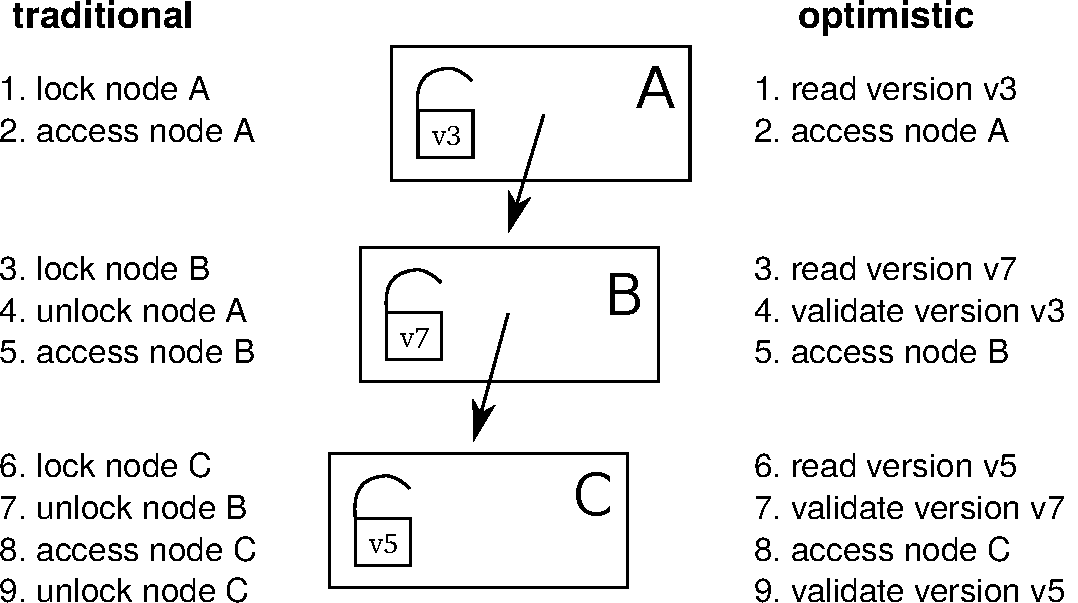
\includegraphics[width=0.65\linewidth]{olcall.pdf}
  \vspace{0.2cm}
  \caption{Comparison of a lookup operation in a 3-level tree using traditional lock coupling (left-hand side) vs.~optimistic lock coupling (right-hand side).}
  \label{fig:olc}
\end{figure}

The traditional and most common lock-based synchronization protocol for B-trees is lock coupling, which interleaves lock acquisitions while holding at most two locks at a time.
If, as we observed earlier, optimistic locks have similar semantics as traditional locks, it is natural to ask whether lock coupling can be combined with optimistic locks.
And indeed the answer is yes: One can almost mechanically translate traditional lock coupling code to optimistic lock coupling code.
This is illustrated in Figure~\ref{fig:olc}, which compares the traversal in a tree of height 3 using traditional and optimistic locks.
As the figure shows, the main difference is that locking is translated to reading the version and that unlocking becomes validation of the previously read version.
This simple change provides efficient lock-free tree traversal without the need to design a complex synchronization protocol.

It is important to emphasize the conceptual simplicity of OLC in comparison to data structures that use custom protocols like the Bw-tree~\cite{DBLP:conf/icde/LevandoskiLS13a}.
To implement lock-free access, the Bw-tree requires an indirection table, delta nodes, complex splitting and merging logic, retry logic, etc.
OLC, on the other hand, can directly be applied to B-trees mostly by adding the appropriate optimistic locking code and without modifying the node layout itself.
Therefore, OpenBw-Tree, an open source implementation of the Bw-tree, requires an order of magnitude more code than a B-tree based on OLC\footnote{Both implementations are available on GitHub: \url{https://github.com/wangziqi2016/index-microbench}}.
Given how difficult it is to develop, validate, and debug lock-free code, simplicity is obviously a major advantage.

\subsection{Correctness Aspects}

\begin{figure}
  % \centering
  %[basicstyle=\normalsize\ttfamily,showstringspaces=false,columns=fullflexible,breaklines=false,breakatwhitespace=true,numbers=none,numberstyle=\small,style=C,keepspaces=true]
\begin{lstlisting}[basicstyle=\ttfamily,language=C++,numbers=left,numberstyle=\small]
std::atomic<BTreeNode*> root;

// search for key in B+tree, returns payload in resultOut
bool lookup(Key key, Value& resultOut) {
   BTreeNode* node = root.load();
   uint64_t nodeVersion = node->readLockOrRestart();
   if (node != root.load()) // make sure the root is still the root
      restart();

   BTreeInner<Key>* parent = nullptr;
   uint64_t parentVersion = 0;

   while (node->isInner()) {
      auto inner = (BTreeInner*)node;

      // unlock parent and make current node the parent
      if (parent)
         parent->readUnlockOrRestart(parentVersion);
      parent = inner;
      parentVersion = nodeVersion;

      // search for next node
      node = inner->findChild(key);
      // validate 'inner' to ensure that 'node' pointer is valid
      inner->checkOrRestart(nodeVersion);
      // now it safe to dereference 'node' pointer (read its version)
      nodeVersion = node->readLockOrRestart();
   }

   // search in leaf and retrieve payload
   auto leaf = (BTreeLeaf*)node;
   bool success = leaf->findValue(key, resultOut);

   // unlock everything
   if (parent)
      parent->readUnlockOrRestart(parentVersion);
   node->readUnlockOrRestart(nodeVersion);

   return success;
}
\end{lstlisting}
  \vspace{0.2cm}
  \caption{B-tree lookup code using OLC. For simplicity, the restart logic is not shown.}
  \label{fig:lookup}
\end{figure}

So far, we have introduced the high-level ideas behind OLC and have stressed its similarity to traditional lock coupling.
Let us now discuss some cases where the close similarity between lock coupling and OLC breaks down.
To make this more concrete, we show the B-tree lookup code in Figure~\ref{fig:lookup}.
In the code, \texttt{readLockOrRestart} reads the lock version and \texttt{readUnlockOrRestart} validates that the read was correct.

One issue with OLC is that any pointer speculatively read from a node may point to invalid memory (if that node is modified concurrently).
Dereferencing such a pointer (e.g., to read its optimistic lock), may cause a segmentation fault or undefined behavior.
In the code shown in Figure~\ref{fig:lookup}, this problem is prevented by the extra check in line 25, which ensures that the read from the node containing the pointer was correct.
Without this additional validation, the code would in line 27 dereference the pointer speculatively read in line 23.
Note that the implementation of \texttt{checkOrRestart} is actually identical to \texttt{readUnlockOrRestart}.
We chose to give it a different name to highlight the fact that this extra check would not be necessary with read/write locks.

Another potential issue with optimistic locks is code that does not terminate.
Code that speculatively accesses a node, like an intra-node binary search, should be written in a way such that it always terminates---even in the presence of concurrent writes.
Otherwise, the validation code that detects the concurrent write will never run.
The binary search of a B-tree, for example, needs to be written in such a way that each comparison makes progress.
For some data structures that do not require loops in the traversal code (like ART) termination is trivially true.

\subsection{Implementation Details}

% implementation, efficiency
To implement an optimistic lock, one can combine the lock and the version counter into a single 64-bit\footnote{Even after subtracting one bit for the lock status, a back-of-the-envelope calculation can show that 63 bits are large enough to never overflow in practice.} word~\cite{artsync}.
A typical read operation will therefore merely consist of reading this version counter atomically.
In C++11 this can be implemented using the \texttt{std::atomic} type.

On x86, atomic reads are cheap because of x86's strong memory order guarantees.
No memory fences are required for sequentially-consistent loads, which are translated (by both GCC and clang) into standard \texttt{MOV} instructions.
Hence, the only effect of \texttt{std::atomic} for loads is preventing instruction re-ordering.
This makes version access and validation cheap.
Acquiring and releasing an optimistic lock in exclusive mode has comparable cost to a traditional lock:
A fairly expensive sequentially-consistent store is needed for acquiring a lock, while a standard \texttt{MOV} suffices for releasing it.
A simple sinlock-based implementation of optimistic locks can be found in the appendix of an earlier paper~\cite{artsync}.

OLC code must be able to handle restarts since validation or lock upgrade can fail due to concurrent writers.
Restarts can easily be implemented by wrapping the data structure operation in a loop (for simplicity not shown in Figure~\ref{fig:lookup}).
Such a loop also enables limiting the number of optimistic retry operations and falling back to pessimistic locking in cases of very heavy contention.
The ability to fall back to traditional locking is a major advantage of OLC in terms of robustness over lock-free approaches, which do not have this option.

In addition to the optimistic shared mode and the exclusive mode, optimistic locks also support a ``shared pessimistic'' mode, which physically acquires the lock in shared mode (allowing multiple concurrent readers but no writers).
This mode is useful for table (or range) scans that touch many tuples on a leaf page (which would otherwise easily abort).
Finally, let us mention that large range scans and table scans, should be broken up into several per-node traversals as is done in the LeanStore~\cite{leanstore} system.

Like all lock-free data structures, but unlike traditional locking and Hardware Transactional Memory~\cite{DBLP:conf/hpca/KarnagelDRLLSL14,DBLP:journals/pvldb/MakreshanskiLS15,htmtkde}, OLC requires care when deleting (and reusing) nodes.
The reason is that a deleting thread can never be sure that a node can be reclaimed because other threads might still be optimistically reading from that node.
Therefore, standard solutions like epoch-based reclamation~\cite{DBLP:conf/sosp/TuZKLM13}, hazard pointers~\cite{DBLP:journals/tpds/Michael04}, or optimized hazard pointers~\cite{DBLP:conf/spaa/BalmauGHZ16} need to be used.
These memory reclamation techniques are, however, largely orthogonal to the synchronization protocol itself.

%-lock-free is not a strong guarantee

\newpage
\section{Evaluation}\label{sec:evaluation}

Let us now experimentally evaluate the overhead and scalability of OLC.
For the experiments, we use an in-memory B+tree implemented in C++11 using templates, which is configured to use nodes of 4096 bytes, random 8 byte keys, and 8 byte payloads.
Based on this B-tree, we compare the following synchronization approaches:
\begin{itemize}
\item an OLC implementation\footnote{An almost identical OLC implementation is available on github: \url{https://github.com/wangziqi2016/index-microbench/tree/master/BTreeOLC}}
\item a variant based on traditional lock coupling and read/write locks
\item the unsynchronized B-tree, which obviously is only correct for read-only workloads but allows measuring the overhead of synchronization
\end{itemize}
Note that earlier work has compared the OLC implementation with a Bw-tree implementation~\cite{buzzword} and other state-of-the-art in-memory index structures.

We use a Haswell EP system with an Intel Xeon E5-2687W v3 CPU, which has 10 cores (20 ``Hyper-Threads'') and 25~MB of L3 cache.
The system is running Ubuntu 18.10 and we use GCC 8.2.0 to compile our code.
The CPU counters are obtained using the Linux perf API\footnote{We use the following convenience wrapper: \url{https://github.com/viktorleis/perfevent}}.

\begin{table}
  \caption{Performance and CPU counters for lookup and insert operations in a B-tree with 100M keys. We perform 100M operations and normalize the CPU counters by that number.}
  \label{tab:overhead}
  \centering
  \begin{tabular}{lrrrrrrr}\toprule
                    &         &        &        & instruc-  & L1     & L3     & branch \\
                    & threads & M op/s & cycles & tions & misses & misses & misses \\\midrule
lookup (no sync.)   & 1       & 1.72   & 2028   & 283     & 39.1   & 14.9   & 16.1   \\
lookup (OLC)        & 1       & 1.65   & 2107   & 370     & 43.9   & 15.1   & 16.7   \\
lookup (lock coup.) & 1       & 1.72   & 2078   & 365     & 42.3   & 16.9   & 15.7   \\\midrule
insert (no sync.)   & 1       & 1.51   & 2286   & 530     & 59.8   & 31.1   & 17.3   \\
insert (OLC)        & 1       & 1.50   & 2303   & 629     & 61.2   & 31.1   & 16.5   \\
insert (lock coup.) & 1       & 1.41   & 2473   & 644     & 61.0   & 31.0   & 17.2   \\\midrule
lookup (no sync.)   & 10      & 15.48  & 2058   & 283     & 38.6   & 15.5   & 16.0   \\
lookup (OLC)        & 10      & 14.60  & 2187   & 370     & 43.8   & 15.8   & 16.8   \\
lookup (lock coup.) & 10      & 5.71   & 5591   & 379     & 54.2   & 17.0   & 14.8   \\\midrule
insert (no sync.)   & 10      & -      & -      & -       & -      & -      & -      \\
insert (OLC)        & 10      & 10.46  & 2940   & 656     & 62.0   & 32.5   & 16.8   \\
insert (lock coup.) & 10      & 7.55   & 4161   & 667     & 75.0   & 28.6   & 16.2   \\
    \bottomrule
\end{tabular}
\end{table}

Table~\ref{tab:overhead} compares the performance and CPU counters for lookup and insert operations in a B-tree with 100M keys.
With {\em single-threaded} execution, we observe that all three approaches have very similar performance.
Adding traditional or optimistic locks to unsynchronized B-tree code results in up to 30\% of additional instructions without affecting single-threaded performance much.

\begin{figure}
  \centering
  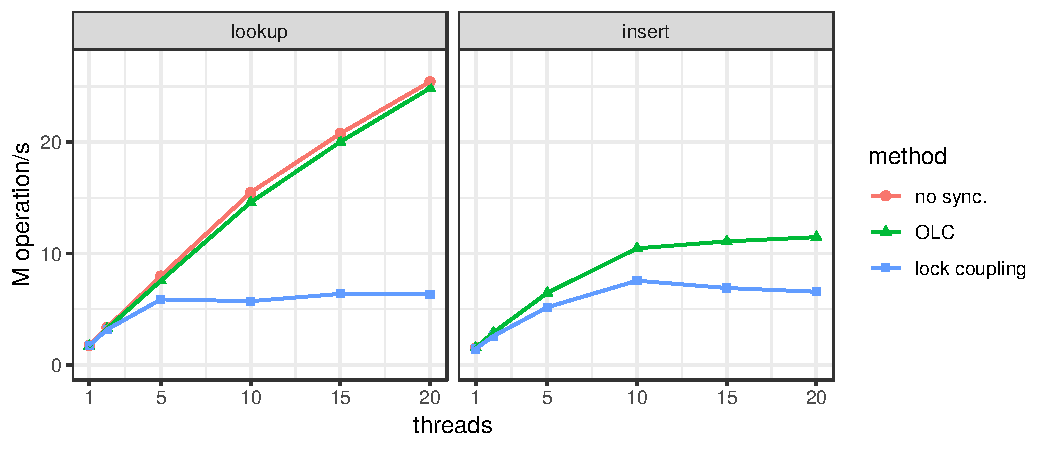
\includegraphics[width=\linewidth]{scale.pdf}
  \vspace{0.2cm}
  \caption{Scalability on 10-core system for B-tree operations (100M values).}
  \label{fig:scale}
\end{figure}

As Figure~\ref{fig:scale} shows, the results change dramatically once we use multiple threads.
For lookup, the scalability of OLC is near-linear up to 20 threads, even though the system has only 10 ``real cores''.
The OLC scalability for insert is also respectable (though not quite as linear because multi-threaded insertion approaches the memory bandwidth of our processor).
The figure also shows that the results of traditional lock coupling with read/write locks are significantly worse than OLC.
With 20 threads, lookup with OLC is 3.9$\times$ faster than traditional lock coupling.

\section{Summary}\label{sec:conc}

Optimistic Lock Coupling (OLC) is an effective synchronization method that combines the simplicity of traditional lock coupling with the superior scalability of lock-free approaches.
OLC is widely applicable and has already been successfully used to synchronize several data structures, including B-trees, binary search trees, and different trie variants.
These features make it highly attractive for modern database systems as well as performance-critical systems software in general.

\begin{thebibliography}{10}

\bibitem{DBLP:conf/spaa/BalmauGHZ16}
O.~Balmau, R.~Guerraoui, M.~Herlihy, and I.~Zablotchi.
\newblock Fast and robust memory reclamation for concurrent data structures.
\newblock In {\em SPAA}, 2016.

\bibitem{DBLP:journals/acta/BayerS77}
R.~Bayer and M.~Schkolnick.
\newblock Concurrency of operations on {B}-trees.
\newblock {\em Acta Informatica}, 9, 1977.

\bibitem{hot}
R.~Binna, E.~Zangerle, M.~Pichl, G.~Specht, and V.~Leis.
\newblock {HOT}: A height optimized trie index for main-memory database
  systems.
\newblock In {\em SIGMOD}, 2018.

\bibitem{DBLP:conf/ppopp/BronsonCCO10}
N.~G. Bronson, J.~Casper, H.~Chafi, and K.~Olukotun.
\newblock A practical concurrent binary search tree.
\newblock In {\em PPOPP}, 2010.

\bibitem{DBLP:conf/vldb/ChaHKK01}
S.~K. Cha, S.~Hwang, K.~Kim, and K.~Kwon.
\newblock Cache-conscious concurrency control of main-memory indexes on
  shared-memory multiprocessor systems.
\newblock In {\em VLDB}, 2001.

\bibitem{intel}
I.~Cutress.
\newblock {Intel} goes for 48-cores: {Cascade-AP} with multi-chip package
  coming soon.
\newblock
  \url{https://www.anandtech.com/show/13535/intel-goes-for-48cores-cascade-ap},
  2018 (accessed January, 2019).

\bibitem{DBLP:conf/cidr/FaleiroA17}
J.~M. Faleiro and D.~J. Abadi.
\newblock Latch-free synchronization in database systems: Silver bullet or
  fool's gold?
\newblock In {\em CIDR}, 2017.

\bibitem{DBLP:journals/ftdb/Graefe11}
G.~Graefe.
\newblock Modern {B}-tree techniques.
\newblock {\em Foundations and Trends in Databases}, 3(4), 2011.

\bibitem{DBLP:conf/hpca/KarnagelDRLLSL14}
T.~Karnagel, R.~Dementiev, R.~Rajwar, K.~Lai, T.~Legler, B.~Schlegel, and
  W.~Lehner.
\newblock Improving in-memory database index performance with
  {Intel}\({}^{\mbox{{\textregistered}}}\) transactional synchronization
  extensions.
\newblock In {\em HPCA}, 2014.

\bibitem{DBLP:journals/tods/LehmanY81}
P.~L. Lehman and S.~B. Yao.
\newblock Efficient locking for concurrent operations on {B}-trees.
\newblock {\em {ACM} Trans. Database Syst.}, 6(4), 1981.

\bibitem{leanstore}
V.~Leis, M.~Haubenschild, A.~Kemper, and T.~Neumann.
\newblock Leanstore: In-memory data management beyond main memory.
\newblock In {\em ICDE}, 2018.

\bibitem{art}
V.~Leis, A.~Kemper, and T.~Neumann.
\newblock The adaptive radix tree: {ARTful} indexing for main-memory databases.
\newblock In {\em ICDE}, 2013.

\bibitem{htmtkde}
V.~Leis, A.~Kemper, and T.~Neumann.
\newblock Scaling {HTM}-supported database transactions to many cores.
\newblock {\em {IEEE} Trans. Knowl. Data Eng.}, 28(2), 2016.

\bibitem{artsync}
V.~Leis, F.~Scheibner, A.~Kemper, and T.~Neumann.
\newblock The {ART} of practical synchronization.
\newblock In {\em DaMoN}, 2016.

\bibitem{DBLP:conf/icde/LevandoskiLS13a}
J.~J. Levandoski, D.~B. Lomet, and S.~Sengupta.
\newblock The {Bw}-tree: A {B}-tree for new hardware platforms.
\newblock In {\em ICDE}, 2013.

\bibitem{DBLP:journals/pvldb/MakreshanskiLS15}
D.~Makreshanski, J.~J. Levandoski, and R.~Stutsman.
\newblock To lock, swap, or elide: On the interplay of hardware transactional
  memory and lock-free indexing.
\newblock {\em {PVLDB}}, 8(11), 2015.

\bibitem{DBLP:dblp_conf/eurosys/MaoKM12}
Y.~Mao, E.~Kohler, and R.~T. Morris.
\newblock Cache craftiness for fast multicore key-value storage.
\newblock In {\em EuroSys}, 2012.

\bibitem{DBLP:journals/tpds/Michael04}
M.~M. Michael.
\newblock Hazard pointers: Safe memory reclamation for lock-free objects.
\newblock {\em {IEEE} Trans. Parallel Distrib. Syst.}, 15(6), 2004.

\bibitem{DBLP:journals/jacm/ShalevS06}
O.~Shalev and N.~Shavit.
\newblock Split-ordered lists: Lock-free extensible hash tables.
\newblock {\em J. {ACM}}, 53(3), 2006.

\bibitem{amd}
A.~Shilov.
\newblock {AMD} previews {EPYC} ‘{Rome}’ processor: Up to 64 {Zen} 2 cores.
\newblock
  \url{https://www.anandtech.com/show/13561/amd-previews-epyc-rome-processor-up-to-64-zen-2-cores},
  2018 (accessed January, 2019).

\bibitem{DBLP:conf/sosp/TuZKLM13}
S.~Tu, W.~Zheng, E.~Kohler, B.~Liskov, and S.~Madden.
\newblock Speedy transactions in multicore in-memory databases.
\newblock In {\em SOSP}, 2013.

\bibitem{buzzword}
Z.~Wang, A.~Pavlo, H.~Lim, V.~Leis, H.~Zhang, M.~Kaminsky, and D.~Andersen.
\newblock Building a {Bw}-tree takes more than just buzz words.
\newblock In {\em SIGMOD}, 2018.

\end{thebibliography}


%\bibliographystyle{abbrv}
%\bibliography{main}

\end{document}

%\end{article}
%
%\begin{article}
%{Interaction Management in Crowdsourcing}
%{Yansheng Wang, Tianshu Song, Qian Tao, Yuxiang Zeng, Zimu Zhou,
%Yi Xu, Yongxin Tong, Lei Chen}
%\graphicspath{{submissions/yongxin}}
%\pdfminorversion=5
\documentclass[11pt]{article}
\usepackage{deauthor,times,graphicx,caption,microtype}
\usepackage{hyperref}
\usepackage{listings}
\usepackage{booktabs}

\begin{document}

\title{Optimistic Lock Coupling: A Scalable and Efficient General-Purpose Synchronization Method}

\author{Viktor Leis, Michael Haubenschild\raisebox{0.9ex}{$\ast$}, Thomas Neumann\\ Technische Universit{\"a}t M{\"u}nchen \hspace{0.7cm} Tableau Software\raisebox{0.9ex}{$\ast$} \\ {\{leis,neumann\}{@}in.tum.de} \hspace{0.7cm} {mhaubenschild{@}tableau.com\raisebox{0.9ex}{$\ast$}}}

\maketitle

\begin{abstract}
As the number of cores on commodity processors continues to increase, scalability becomes more and more crucial for overall performance.
Scalable and efficient concurrent data structures are particularly important, as these are often the building blocks of parallel algorithms.
Unfortunately, traditional synchronization techniques based on fine-grained locking have been shown to be unscalable on modern multi-core CPUs.
Lock-free data structures, on the other hand, are extremely difficult to design and often incur significant overhead.

In this work, we make the case for Optimistic Lock Coupling as a practical alternative to both traditional locking and the lock-free approach.
We show that Optimistic Lock Coupling is highly scalable and almost as simple to implement as traditional lock coupling.
Another important advantage is that it is easily applicable to most tree-like data structures.
We therefore argue that Optimistic Lock Coupling, rather than a complex and error-prone custom synchronization protocol, should be the default choice for performance-critical data structures.
\end{abstract}

\section{Introduction}

% more and more cores
Today, Intel's commodity server processors have up to 28 cores and its upcoming microarchitecture will have up to 48 cores per socket~\cite{intel}.
Similarly, AMD currently stands at 32 cores and this number is expected to double in the next generation~\cite{amd}.
Since both platforms support simultaneous multithreading (also known as hyperthreading), affordable commodity servers (with up to two sockets) will soon routinely have between 100 and 200 hardware threads.

% data structure scalability is important
With such a high degree of hardware parallelism, efficient data processing crucially depends on how well concurrent data structures scale.
Internally, database systems use a plethora of data structures like table heaps, internal work queues, and, most importantly, index structures.
Any of these can easily become a scalability (and therefore overall performance) bottleneck on many-core CPUs.

% traditional synchronization: fine-grained locks, slow, cache invalidation
Traditionally, database systems synchronize internal data structures using fine-grained reader/writer locks\footnote{In this work, we focus on data structure synchronization rather than high-level transaction semantics and therefore use the term {\em lock} for what would typically be called {\em latch} in the database literature. We thus follow common computer science (rather than database) terminology.}.
Unfortunately, while fine-grained locking makes lock contention unlikely, it still results in bad scalability because lock acquisition and release require writing to shared memory.
Due to the way cache coherency is implemented on modern multi-core CPUs, these writes cause additional cache misses\footnote{The cache coherency protocol ensures that all copies of a cache line on other cores are invalidated before the write can proceed.} and the cache line containing the lock's internal data becomes a point of physical contention.
As a result, any frequently-accessed lock (e.g., the lock of the root node of a B-tree) severely limits scalability.

% lock-free bw-tree: no more latches, but indirections, extremely complex
Lock-free data structures like the Bw-tree~\cite{DBLP:conf/icde/LevandoskiLS13a} (a lock-free B-tree variant) or the Split-Ordered List~\cite{DBLP:journals/jacm/ShalevS06} (a lock-free hash table) do not acquire any locks and therefore generally scale much better than locking-based approaches (in particular for read-mostly workloads).
However, lock-free synchronization has other downsides:
First, it is very difficult and results in extremely complex and error-prone code (when compared to locking).
Second, because the functionality of atomic primitives provided by the hardware (e.g., atomically compare-and-swap 8 bytes) is limited, complex operations require additional indirections within the data structure.
For example, the Bw-tree requires an indirection table and the Split-Ordered List requires ``dummy nodes'', resulting in overhead due to additional cache misses.

% OLC for the win
In this paper we make the case for {\em Optimistic Lock Coupling (OLC)}, a synchronization method that combines some of the best properties of lock-based and lock-free synchronization.
OLC utilizes a special lock type that can be used in two modes:
The first mode is similar to a traditional mutex and excludes other threads by physically acquiring the underlying lock.
In the second mode, reads can proceed optimistically by validating a version counter that is embedded in the lock (similar to optimistic concurrency control).
The first mode is typically used by writers and the second mode by readers.
Besides this special lock type, OLC is based on the observation that optimistic lock validations can be interleaved/coupled---similar to the pair-wise interleaved lock acquisition of traditional lock coupling.
Hence, the name Optimistic Lock Coupling.

OLC has a number of desirable features:
\begin{itemize}
\item By reducing the number of writes to shared memory locations and thereby avoiding cache invalidations, it {\bf scales well} for most workloads.
\item In comparison to unsynchronized code, it requires few additional CPU instructions making it {\bf efficient}.
\item OLC is {\bf widely applicable} to different data structures. It has already been successfully used for synchronizing binary search trees~\cite{DBLP:conf/ppopp/BronsonCCO10}, tries~\cite{artsync}, trie/B-tree hybrids~\cite{DBLP:dblp_conf/eurosys/MaoKM12}, and B-trees~\cite{buzzword}.
\item In comparison to the lock-free paradigm, it is also {\bf easy to use} and requires few modifications to existing, single-threaded data structures.
\end{itemize}
Despite these positive features and its simplicity, OLC is not yet widely known.
The goal of this paper is therefore to popularize this simple idea and to make a case for it.
We argue that OLC deserves to be widely known.
It is a good default synchronization paradigm---more complex, data structure-specific protocols are seldom beneficial.

The rest of the paper is organized as follows.
Section~\ref{sec:related} discusses related work, tracing the history of OLC and its underlying ideas in the literature.
The core of the paper is Section~\ref{sec:olc}, which describes the ideas behind OLC and how it can be used to synchronize complex data structures.
In Section~\ref{sec:evaluation} we experimentally show that OLC has low overhead and scales well when used to synchronize an in-memory B-tree.
We summarize the paper in Section~\ref{sec:conc}.

\newpage
\section{Related Work}\label{sec:related}

Lock coupling has been proposed as a method for allowing concurrent operations on B-trees in 1977~\cite{DBLP:journals/acta/BayerS77}.
This traditional and still widely-used method, described in detail in Graefe's B-tree survey~\cite{DBLP:journals/ftdb/Graefe11}, is also called ``latch coupling'', ``hand-over-hand locking'', and ``crabbing''.
Because at most two locks are held at-a-time during tree traversal, this technique seemingly allows for a high degree of parallelism---in particular if read/write locks are used to enable inner nodes to be locked in shared mode.
However, as we show in Section~\ref{sec:evaluation}, on modern hardware lock acquisition (even in shared mode) results in suboptimal scalability.

An early alternative from 1981 is a B-tree variant called B-link tree~\cite{DBLP:journals/tods/LehmanY81}, which only holds a single lock at a time.
It is based on the observation that between the release of the parent lock and the acquisition of the child lock, the only ``dangerous'' thing that could have happened is the split of a child node (assuming one does not implement merge operations).
Thus, when a split happens, the key being searched might end up on a neighboring node to the right of the current child node.
A B-link tree traversal therefore detects this condition and, if needed, transparently proceeds to the neighboring node.
Releasing the parent lock early is highly beneficial when the child node needs to be fetched from disk.
For in-memory workloads, however, the B-link tree has the same scalability issues as lock coupling (it acquires just as many locks).

The next major advance, Optimistic Latch-Free Index Traversal (OLFIT)~\cite{DBLP:conf/vldb/ChaHKK01}, was proposed in 2001.
OLFIT introduced the idea of a combined lock/update counter, which we call {\em optimistic lock}. % , for lack of a better name,
Based on these per-node optimistic locks and the synchronization protocol of the B-link tree, OLFIT finally achieves good scalability on parallel processors.
The OLFIT protocol is fairly complex, as it requires both the non-trivial B-link protocol and optimistic locks.
Furthermore, like the B-link tree protocol, it does not support merging nodes, and is specific to B-trees (cannot easily be applied to other data structures).

In the following two decades, the growth of main-memory capacity led to much research into other data structures besides the venerable B-tree.
Particularly relevant for our discussion is Bronson et al.'s~\cite{DBLP:conf/ppopp/BronsonCCO10} concurrent binary search tree, which is based on optimistic version validation and has a sophisticated, data structure-specific synchronization protocol.
To the best of our knowledge, this 2010 paper is the first that, as part of its protocol, interleaves version validation across nodes---rather than validating each node separately like OLFIT.
In that paper, this idea is called ``hand-over-hand, optimistic validation'', while we prefer the term Optimistic Lock Coupling to highlight the close resemblance to traditional lock coupling.
Similarly, Mao et al.'s~\cite{DBLP:dblp_conf/eurosys/MaoKM12} Masstree (a concurrent hybrid trie/B-tree) is also based on the same ideas, but again uses them as part of a more complex protocol.

The Adaptive Radix Tree (ART)~\cite{art} is another recent in-memory data structure, which we proposed in 2013.
In contrast to the two data structures just mentioned, it was originally designed with single-threaded performance in mind without supporting concurrency.
To add support for concurrency, we initially started designing a custom protocol called Read-Optimized Write Exclusion (ROWEX)~\cite{artsync}, which turned out to be non-trivial and requires modifications of the underlying data structure\footnote{Note that ROWEX is already easier to apply to existing data structures than the lock-free approach. The difficulty depends on the data structure. Applying ROWEX is hard for B-trees with sorted keys and fairly easy for copy-on-write data structures like the Height Optimized Trie~\cite{hot}---with ART being somewhere in the middle.}.
However, fairly late in the project, we also realized, that OLC {\em alone} (rather than as part of a more complex protocol) is sufficient to synchronize ART.
No other changes to the data structure were necessary.
Both approaches were published and experimentally evaluated in a followup paper~\cite{artsync}, which shows that, despite its simplicity, OLC is efficient, scalable, and generally outperforms ROWEX.

Similar results were recently published regarding B-trees~\cite{buzzword}.
In this experimental study a simple OLC-based synchronization outperformed the Bw-tree~\cite{DBLP:conf/icde/LevandoskiLS13a}, a complex lock-free synchronization approach.
Another recent paper shows that for write-intensive workloads, locking often performs better than lock-free synchronization~\cite{DBLP:conf/cidr/FaleiroA17}.
These experiences indicate that OLC is a general-purpose synchronization paradigm and motivate the current paper.

%foster b-tree\cite{DBLP:journals/tods/GraefeKK12}
%Shasha theory~\cite{DBLP:journals/tods/ShashaG88}

\section{Optimistic Lock Coupling}\label{sec:olc}

% locks suck
The standard technique for inter-thread synchronization is mutual exclusion using fine-grained locks.
In a B-tree, for example, every node usually has its own associated lock, which is acquired before accessing that node.
The problem of locking on modern multi- and many-core processors is that lock acquisition and release require writing to the shared memory location that implements the lock.
This write causes exclusive ownership of the underlying cache line and invalidates copies of it on all other processor cores.
For hierarchical, tree-like data structures, the lock of the root node becomes a point of physical contention---even in read-only workloads and even when read/write locks are used.
Depending on the specific data structure, number of cores, cache coherency protocol implementation, cache topology, whether Non-Uniform Memory Access (NUMA) is used, locking can even result in multi-threaded performance that is worse than single-threaded execution.

% in b-trees this happens very much
The inherent pessimism of locking is particularly unfortunate for B-trees:
Despite the fact that logical modifications of the root node are very infrequent, every B-tree operation must lock the root node during tree traversal\footnote{To a lesser extent this obviously applies to all inner nodes, not just the root.}.
Even the vast majority of update operations (with the exception of splits and merges), only modify a single leaf node.
These observations indicate that a more optimistic approach, which does not require locking inner nodes, would be very beneficial for B-trees.

\subsection{Optimistic Locks}

% optimism to the rescue
As the name indicates, optimistic locks try to solve the scalability issues of traditional locks using an optimistic approach.
Instead of always physically acquiring locks, even for nodes that are unlikely to be modified simultaneously, after-the-fact validation is used to detect conflicts.
This is done by augmenting each lock with a version/update counter that is incremented on every modification.
Using this version counter, readers can optimistically proceed before validating that the version did not change to ensure that the read was safe.
If validation fails, the operation is restarted.

% details on opt locks
Using optimistic locks, a read-only node access (i.e., the majority of all operations in a B-tree) does not acquire the lock and does not increment the version counter.
Instead, it performs the following steps:
\begin{enumerate}
\item read lock version (restart if lock is not free)
\item access node
\item read the version again and validate that it has not changed in the meantime
\end{enumerate}
If the last step (the validation) fails, the operation has to be restarted.
Write operations, on the other hand, are more similar to traditional locking:
\begin{enumerate}
\item acquire lock (wait if necessary)
\item access/write to node
\item increment version and unlock node
\end{enumerate}
Writes can therefore protect a node from other writes.

% similar to locks
As we observed in an earlier paper~\cite{artsync}, because of similar semantics, optimistic locks can be hidden behind an API very similar to traditional read/write locks.
Both approaches have an exclusive lock mode, and acquiring a traditional lock in shared mode is analogous to optimistic version validation.
Furthermore, like with some implementations of traditional read/write locks, optimistic locks allow upgrading a shared lock to an exclusive lock.
Lock upgrades are, for example, used to avoid most B-tree update operations from having to lock inner nodes.
In our experience, the close resemblance of optimistic and traditional locks simplifies the reasoning about optimistic locks;
one can apply similar thinking as in traditional lock-based protocols.

\subsection{Lock Coupling with Optimistic Locks}

\begin{figure}
  \centering
  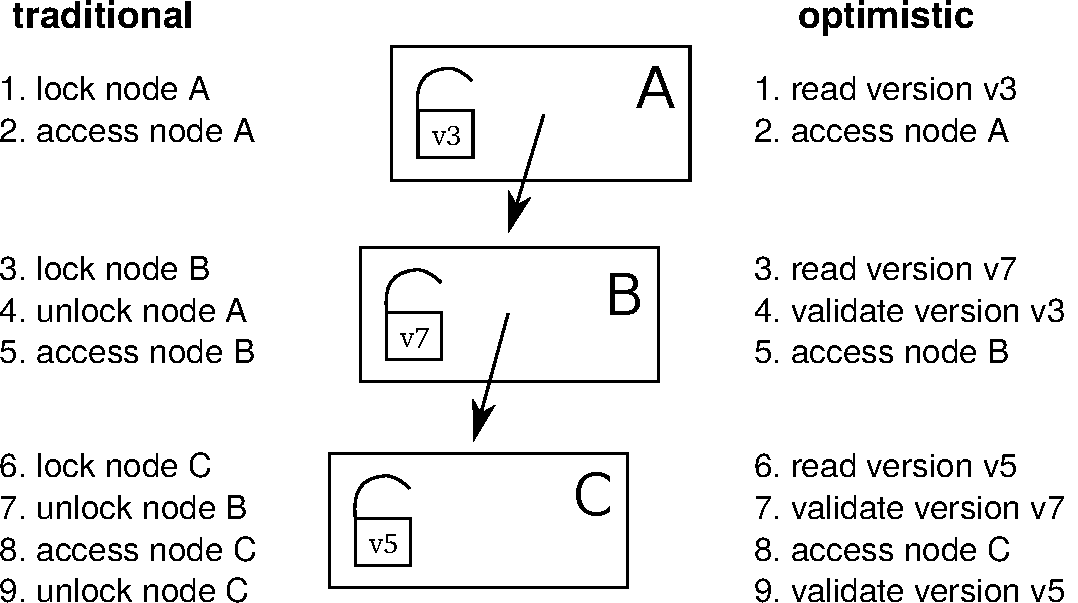
\includegraphics[width=0.65\linewidth]{olcall.pdf}
  \vspace{0.2cm}
  \caption{Comparison of a lookup operation in a 3-level tree using traditional lock coupling (left-hand side) vs.~optimistic lock coupling (right-hand side).}
  \label{fig:olc}
\end{figure}

The traditional and most common lock-based synchronization protocol for B-trees is lock coupling, which interleaves lock acquisitions while holding at most two locks at a time.
If, as we observed earlier, optimistic locks have similar semantics as traditional locks, it is natural to ask whether lock coupling can be combined with optimistic locks.
And indeed the answer is yes: One can almost mechanically translate traditional lock coupling code to optimistic lock coupling code.
This is illustrated in Figure~\ref{fig:olc}, which compares the traversal in a tree of height 3 using traditional and optimistic locks.
As the figure shows, the main difference is that locking is translated to reading the version and that unlocking becomes validation of the previously read version.
This simple change provides efficient lock-free tree traversal without the need to design a complex synchronization protocol.

It is important to emphasize the conceptual simplicity of OLC in comparison to data structures that use custom protocols like the Bw-tree~\cite{DBLP:conf/icde/LevandoskiLS13a}.
To implement lock-free access, the Bw-tree requires an indirection table, delta nodes, complex splitting and merging logic, retry logic, etc.
OLC, on the other hand, can directly be applied to B-trees mostly by adding the appropriate optimistic locking code and without modifying the node layout itself.
Therefore, OpenBw-Tree, an open source implementation of the Bw-tree, requires an order of magnitude more code than a B-tree based on OLC\footnote{Both implementations are available on GitHub: \url{https://github.com/wangziqi2016/index-microbench}}.
Given how difficult it is to develop, validate, and debug lock-free code, simplicity is obviously a major advantage.

\subsection{Correctness Aspects}

\begin{figure}
  % \centering
  %[basicstyle=\normalsize\ttfamily,showstringspaces=false,columns=fullflexible,breaklines=false,breakatwhitespace=true,numbers=none,numberstyle=\small,style=C,keepspaces=true]
\begin{lstlisting}[basicstyle=\ttfamily,language=C++,numbers=left,numberstyle=\small]
std::atomic<BTreeNode*> root;

// search for key in B+tree, returns payload in resultOut
bool lookup(Key key, Value& resultOut) {
   BTreeNode* node = root.load();
   uint64_t nodeVersion = node->readLockOrRestart();
   if (node != root.load()) // make sure the root is still the root
      restart();

   BTreeInner<Key>* parent = nullptr;
   uint64_t parentVersion = 0;

   while (node->isInner()) {
      auto inner = (BTreeInner*)node;

      // unlock parent and make current node the parent
      if (parent)
         parent->readUnlockOrRestart(parentVersion);
      parent = inner;
      parentVersion = nodeVersion;

      // search for next node
      node = inner->findChild(key);
      // validate 'inner' to ensure that 'node' pointer is valid
      inner->checkOrRestart(nodeVersion);
      // now it safe to dereference 'node' pointer (read its version)
      nodeVersion = node->readLockOrRestart();
   }

   // search in leaf and retrieve payload
   auto leaf = (BTreeLeaf*)node;
   bool success = leaf->findValue(key, resultOut);

   // unlock everything
   if (parent)
      parent->readUnlockOrRestart(parentVersion);
   node->readUnlockOrRestart(nodeVersion);

   return success;
}
\end{lstlisting}
  \vspace{0.2cm}
  \caption{B-tree lookup code using OLC. For simplicity, the restart logic is not shown.}
  \label{fig:lookup}
\end{figure}

So far, we have introduced the high-level ideas behind OLC and have stressed its similarity to traditional lock coupling.
Let us now discuss some cases where the close similarity between lock coupling and OLC breaks down.
To make this more concrete, we show the B-tree lookup code in Figure~\ref{fig:lookup}.
In the code, \texttt{readLockOrRestart} reads the lock version and \texttt{readUnlockOrRestart} validates that the read was correct.

One issue with OLC is that any pointer speculatively read from a node may point to invalid memory (if that node is modified concurrently).
Dereferencing such a pointer (e.g., to read its optimistic lock), may cause a segmentation fault or undefined behavior.
In the code shown in Figure~\ref{fig:lookup}, this problem is prevented by the extra check in line 25, which ensures that the read from the node containing the pointer was correct.
Without this additional validation, the code would in line 27 dereference the pointer speculatively read in line 23.
Note that the implementation of \texttt{checkOrRestart} is actually identical to \texttt{readUnlockOrRestart}.
We chose to give it a different name to highlight the fact that this extra check would not be necessary with read/write locks.

Another potential issue with optimistic locks is code that does not terminate.
Code that speculatively accesses a node, like an intra-node binary search, should be written in a way such that it always terminates---even in the presence of concurrent writes.
Otherwise, the validation code that detects the concurrent write will never run.
The binary search of a B-tree, for example, needs to be written in such a way that each comparison makes progress.
For some data structures that do not require loops in the traversal code (like ART) termination is trivially true.

\subsection{Implementation Details}

% implementation, efficiency
To implement an optimistic lock, one can combine the lock and the version counter into a single 64-bit\footnote{Even after subtracting one bit for the lock status, a back-of-the-envelope calculation can show that 63 bits are large enough to never overflow in practice.} word~\cite{artsync}.
A typical read operation will therefore merely consist of reading this version counter atomically.
In C++11 this can be implemented using the \texttt{std::atomic} type.

On x86, atomic reads are cheap because of x86's strong memory order guarantees.
No memory fences are required for sequentially-consistent loads, which are translated (by both GCC and clang) into standard \texttt{MOV} instructions.
Hence, the only effect of \texttt{std::atomic} for loads is preventing instruction re-ordering.
This makes version access and validation cheap.
Acquiring and releasing an optimistic lock in exclusive mode has comparable cost to a traditional lock:
A fairly expensive sequentially-consistent store is needed for acquiring a lock, while a standard \texttt{MOV} suffices for releasing it.
A simple sinlock-based implementation of optimistic locks can be found in the appendix of an earlier paper~\cite{artsync}.

OLC code must be able to handle restarts since validation or lock upgrade can fail due to concurrent writers.
Restarts can easily be implemented by wrapping the data structure operation in a loop (for simplicity not shown in Figure~\ref{fig:lookup}).
Such a loop also enables limiting the number of optimistic retry operations and falling back to pessimistic locking in cases of very heavy contention.
The ability to fall back to traditional locking is a major advantage of OLC in terms of robustness over lock-free approaches, which do not have this option.

In addition to the optimistic shared mode and the exclusive mode, optimistic locks also support a ``shared pessimistic'' mode, which physically acquires the lock in shared mode (allowing multiple concurrent readers but no writers).
This mode is useful for table (or range) scans that touch many tuples on a leaf page (which would otherwise easily abort).
Finally, let us mention that large range scans and table scans, should be broken up into several per-node traversals as is done in the LeanStore~\cite{leanstore} system.

Like all lock-free data structures, but unlike traditional locking and Hardware Transactional Memory~\cite{DBLP:conf/hpca/KarnagelDRLLSL14,DBLP:journals/pvldb/MakreshanskiLS15,htmtkde}, OLC requires care when deleting (and reusing) nodes.
The reason is that a deleting thread can never be sure that a node can be reclaimed because other threads might still be optimistically reading from that node.
Therefore, standard solutions like epoch-based reclamation~\cite{DBLP:conf/sosp/TuZKLM13}, hazard pointers~\cite{DBLP:journals/tpds/Michael04}, or optimized hazard pointers~\cite{DBLP:conf/spaa/BalmauGHZ16} need to be used.
These memory reclamation techniques are, however, largely orthogonal to the synchronization protocol itself.

%-lock-free is not a strong guarantee

\newpage
\section{Evaluation}\label{sec:evaluation}

Let us now experimentally evaluate the overhead and scalability of OLC.
For the experiments, we use an in-memory B+tree implemented in C++11 using templates, which is configured to use nodes of 4096 bytes, random 8 byte keys, and 8 byte payloads.
Based on this B-tree, we compare the following synchronization approaches:
\begin{itemize}
\item an OLC implementation\footnote{An almost identical OLC implementation is available on github: \url{https://github.com/wangziqi2016/index-microbench/tree/master/BTreeOLC}}
\item a variant based on traditional lock coupling and read/write locks
\item the unsynchronized B-tree, which obviously is only correct for read-only workloads but allows measuring the overhead of synchronization
\end{itemize}
Note that earlier work has compared the OLC implementation with a Bw-tree implementation~\cite{buzzword} and other state-of-the-art in-memory index structures.

We use a Haswell EP system with an Intel Xeon E5-2687W v3 CPU, which has 10 cores (20 ``Hyper-Threads'') and 25~MB of L3 cache.
The system is running Ubuntu 18.10 and we use GCC 8.2.0 to compile our code.
The CPU counters are obtained using the Linux perf API\footnote{We use the following convenience wrapper: \url{https://github.com/viktorleis/perfevent}}.

\begin{table}
  \caption{Performance and CPU counters for lookup and insert operations in a B-tree with 100M keys. We perform 100M operations and normalize the CPU counters by that number.}
  \label{tab:overhead}
  \centering
  \begin{tabular}{lrrrrrrr}\toprule
                    &         &        &        & instruc-  & L1     & L3     & branch \\
                    & threads & M op/s & cycles & tions & misses & misses & misses \\\midrule
lookup (no sync.)   & 1       & 1.72   & 2028   & 283     & 39.1   & 14.9   & 16.1   \\
lookup (OLC)        & 1       & 1.65   & 2107   & 370     & 43.9   & 15.1   & 16.7   \\
lookup (lock coup.) & 1       & 1.72   & 2078   & 365     & 42.3   & 16.9   & 15.7   \\\midrule
insert (no sync.)   & 1       & 1.51   & 2286   & 530     & 59.8   & 31.1   & 17.3   \\
insert (OLC)        & 1       & 1.50   & 2303   & 629     & 61.2   & 31.1   & 16.5   \\
insert (lock coup.) & 1       & 1.41   & 2473   & 644     & 61.0   & 31.0   & 17.2   \\\midrule
lookup (no sync.)   & 10      & 15.48  & 2058   & 283     & 38.6   & 15.5   & 16.0   \\
lookup (OLC)        & 10      & 14.60  & 2187   & 370     & 43.8   & 15.8   & 16.8   \\
lookup (lock coup.) & 10      & 5.71   & 5591   & 379     & 54.2   & 17.0   & 14.8   \\\midrule
insert (no sync.)   & 10      & -      & -      & -       & -      & -      & -      \\
insert (OLC)        & 10      & 10.46  & 2940   & 656     & 62.0   & 32.5   & 16.8   \\
insert (lock coup.) & 10      & 7.55   & 4161   & 667     & 75.0   & 28.6   & 16.2   \\
    \bottomrule
\end{tabular}
\end{table}

Table~\ref{tab:overhead} compares the performance and CPU counters for lookup and insert operations in a B-tree with 100M keys.
With {\em single-threaded} execution, we observe that all three approaches have very similar performance.
Adding traditional or optimistic locks to unsynchronized B-tree code results in up to 30\% of additional instructions without affecting single-threaded performance much.

\begin{figure}
  \centering
  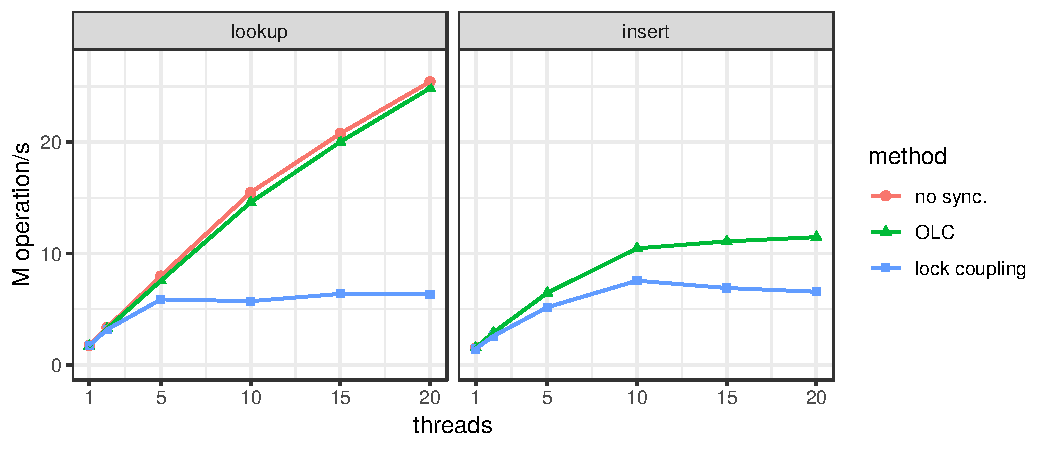
\includegraphics[width=\linewidth]{scale.pdf}
  \vspace{0.2cm}
  \caption{Scalability on 10-core system for B-tree operations (100M values).}
  \label{fig:scale}
\end{figure}

As Figure~\ref{fig:scale} shows, the results change dramatically once we use multiple threads.
For lookup, the scalability of OLC is near-linear up to 20 threads, even though the system has only 10 ``real cores''.
The OLC scalability for insert is also respectable (though not quite as linear because multi-threaded insertion approaches the memory bandwidth of our processor).
The figure also shows that the results of traditional lock coupling with read/write locks are significantly worse than OLC.
With 20 threads, lookup with OLC is 3.9$\times$ faster than traditional lock coupling.

\section{Summary}\label{sec:conc}

Optimistic Lock Coupling (OLC) is an effective synchronization method that combines the simplicity of traditional lock coupling with the superior scalability of lock-free approaches.
OLC is widely applicable and has already been successfully used to synchronize several data structures, including B-trees, binary search trees, and different trie variants.
These features make it highly attractive for modern database systems as well as performance-critical systems software in general.

\begin{thebibliography}{10}

\bibitem{DBLP:conf/spaa/BalmauGHZ16}
O.~Balmau, R.~Guerraoui, M.~Herlihy, and I.~Zablotchi.
\newblock Fast and robust memory reclamation for concurrent data structures.
\newblock In {\em SPAA}, 2016.

\bibitem{DBLP:journals/acta/BayerS77}
R.~Bayer and M.~Schkolnick.
\newblock Concurrency of operations on {B}-trees.
\newblock {\em Acta Informatica}, 9, 1977.

\bibitem{hot}
R.~Binna, E.~Zangerle, M.~Pichl, G.~Specht, and V.~Leis.
\newblock {HOT}: A height optimized trie index for main-memory database
  systems.
\newblock In {\em SIGMOD}, 2018.

\bibitem{DBLP:conf/ppopp/BronsonCCO10}
N.~G. Bronson, J.~Casper, H.~Chafi, and K.~Olukotun.
\newblock A practical concurrent binary search tree.
\newblock In {\em PPOPP}, 2010.

\bibitem{DBLP:conf/vldb/ChaHKK01}
S.~K. Cha, S.~Hwang, K.~Kim, and K.~Kwon.
\newblock Cache-conscious concurrency control of main-memory indexes on
  shared-memory multiprocessor systems.
\newblock In {\em VLDB}, 2001.

\bibitem{intel}
I.~Cutress.
\newblock {Intel} goes for 48-cores: {Cascade-AP} with multi-chip package
  coming soon.
\newblock
  \url{https://www.anandtech.com/show/13535/intel-goes-for-48cores-cascade-ap},
  2018 (accessed January, 2019).

\bibitem{DBLP:conf/cidr/FaleiroA17}
J.~M. Faleiro and D.~J. Abadi.
\newblock Latch-free synchronization in database systems: Silver bullet or
  fool's gold?
\newblock In {\em CIDR}, 2017.

\bibitem{DBLP:journals/ftdb/Graefe11}
G.~Graefe.
\newblock Modern {B}-tree techniques.
\newblock {\em Foundations and Trends in Databases}, 3(4), 2011.

\bibitem{DBLP:conf/hpca/KarnagelDRLLSL14}
T.~Karnagel, R.~Dementiev, R.~Rajwar, K.~Lai, T.~Legler, B.~Schlegel, and
  W.~Lehner.
\newblock Improving in-memory database index performance with
  {Intel}\({}^{\mbox{{\textregistered}}}\) transactional synchronization
  extensions.
\newblock In {\em HPCA}, 2014.

\bibitem{DBLP:journals/tods/LehmanY81}
P.~L. Lehman and S.~B. Yao.
\newblock Efficient locking for concurrent operations on {B}-trees.
\newblock {\em {ACM} Trans. Database Syst.}, 6(4), 1981.

\bibitem{leanstore}
V.~Leis, M.~Haubenschild, A.~Kemper, and T.~Neumann.
\newblock Leanstore: In-memory data management beyond main memory.
\newblock In {\em ICDE}, 2018.

\bibitem{art}
V.~Leis, A.~Kemper, and T.~Neumann.
\newblock The adaptive radix tree: {ARTful} indexing for main-memory databases.
\newblock In {\em ICDE}, 2013.

\bibitem{htmtkde}
V.~Leis, A.~Kemper, and T.~Neumann.
\newblock Scaling {HTM}-supported database transactions to many cores.
\newblock {\em {IEEE} Trans. Knowl. Data Eng.}, 28(2), 2016.

\bibitem{artsync}
V.~Leis, F.~Scheibner, A.~Kemper, and T.~Neumann.
\newblock The {ART} of practical synchronization.
\newblock In {\em DaMoN}, 2016.

\bibitem{DBLP:conf/icde/LevandoskiLS13a}
J.~J. Levandoski, D.~B. Lomet, and S.~Sengupta.
\newblock The {Bw}-tree: A {B}-tree for new hardware platforms.
\newblock In {\em ICDE}, 2013.

\bibitem{DBLP:journals/pvldb/MakreshanskiLS15}
D.~Makreshanski, J.~J. Levandoski, and R.~Stutsman.
\newblock To lock, swap, or elide: On the interplay of hardware transactional
  memory and lock-free indexing.
\newblock {\em {PVLDB}}, 8(11), 2015.

\bibitem{DBLP:dblp_conf/eurosys/MaoKM12}
Y.~Mao, E.~Kohler, and R.~T. Morris.
\newblock Cache craftiness for fast multicore key-value storage.
\newblock In {\em EuroSys}, 2012.

\bibitem{DBLP:journals/tpds/Michael04}
M.~M. Michael.
\newblock Hazard pointers: Safe memory reclamation for lock-free objects.
\newblock {\em {IEEE} Trans. Parallel Distrib. Syst.}, 15(6), 2004.

\bibitem{DBLP:journals/jacm/ShalevS06}
O.~Shalev and N.~Shavit.
\newblock Split-ordered lists: Lock-free extensible hash tables.
\newblock {\em J. {ACM}}, 53(3), 2006.

\bibitem{amd}
A.~Shilov.
\newblock {AMD} previews {EPYC} ‘{Rome}’ processor: Up to 64 {Zen} 2 cores.
\newblock
  \url{https://www.anandtech.com/show/13561/amd-previews-epyc-rome-processor-up-to-64-zen-2-cores},
  2018 (accessed January, 2019).

\bibitem{DBLP:conf/sosp/TuZKLM13}
S.~Tu, W.~Zheng, E.~Kohler, B.~Liskov, and S.~Madden.
\newblock Speedy transactions in multicore in-memory databases.
\newblock In {\em SOSP}, 2013.

\bibitem{buzzword}
Z.~Wang, A.~Pavlo, H.~Lim, V.~Leis, H.~Zhang, M.~Kaminsky, and D.~Andersen.
\newblock Building a {Bw}-tree takes more than just buzz words.
\newblock In {\em SIGMOD}, 2018.

\end{thebibliography}


%\bibliographystyle{abbrv}
%\bibliography{main}

\end{document}

%\end{article}
%
%
%\begin{article}
%{Platform Design for Crowdsourcing and Future of Work}
%{David Gross-Amblard, Atsuyuki Morishima, Saravanan Thirumuruganathan,Marion Tommasi, Ko Yoshida}
%\graphicspath{{submissions/atsuyuki/}}
%\pdfminorversion=5
\documentclass[11pt]{article}
\usepackage{deauthor,times,graphicx,caption,microtype}
\usepackage{hyperref}
\usepackage{listings}
\usepackage{booktabs}

\begin{document}

\title{Optimistic Lock Coupling: A Scalable and Efficient General-Purpose Synchronization Method}

\author{Viktor Leis, Michael Haubenschild\raisebox{0.9ex}{$\ast$}, Thomas Neumann\\ Technische Universit{\"a}t M{\"u}nchen \hspace{0.7cm} Tableau Software\raisebox{0.9ex}{$\ast$} \\ {\{leis,neumann\}{@}in.tum.de} \hspace{0.7cm} {mhaubenschild{@}tableau.com\raisebox{0.9ex}{$\ast$}}}

\maketitle

\begin{abstract}
As the number of cores on commodity processors continues to increase, scalability becomes more and more crucial for overall performance.
Scalable and efficient concurrent data structures are particularly important, as these are often the building blocks of parallel algorithms.
Unfortunately, traditional synchronization techniques based on fine-grained locking have been shown to be unscalable on modern multi-core CPUs.
Lock-free data structures, on the other hand, are extremely difficult to design and often incur significant overhead.

In this work, we make the case for Optimistic Lock Coupling as a practical alternative to both traditional locking and the lock-free approach.
We show that Optimistic Lock Coupling is highly scalable and almost as simple to implement as traditional lock coupling.
Another important advantage is that it is easily applicable to most tree-like data structures.
We therefore argue that Optimistic Lock Coupling, rather than a complex and error-prone custom synchronization protocol, should be the default choice for performance-critical data structures.
\end{abstract}

\section{Introduction}

% more and more cores
Today, Intel's commodity server processors have up to 28 cores and its upcoming microarchitecture will have up to 48 cores per socket~\cite{intel}.
Similarly, AMD currently stands at 32 cores and this number is expected to double in the next generation~\cite{amd}.
Since both platforms support simultaneous multithreading (also known as hyperthreading), affordable commodity servers (with up to two sockets) will soon routinely have between 100 and 200 hardware threads.

% data structure scalability is important
With such a high degree of hardware parallelism, efficient data processing crucially depends on how well concurrent data structures scale.
Internally, database systems use a plethora of data structures like table heaps, internal work queues, and, most importantly, index structures.
Any of these can easily become a scalability (and therefore overall performance) bottleneck on many-core CPUs.

% traditional synchronization: fine-grained locks, slow, cache invalidation
Traditionally, database systems synchronize internal data structures using fine-grained reader/writer locks\footnote{In this work, we focus on data structure synchronization rather than high-level transaction semantics and therefore use the term {\em lock} for what would typically be called {\em latch} in the database literature. We thus follow common computer science (rather than database) terminology.}.
Unfortunately, while fine-grained locking makes lock contention unlikely, it still results in bad scalability because lock acquisition and release require writing to shared memory.
Due to the way cache coherency is implemented on modern multi-core CPUs, these writes cause additional cache misses\footnote{The cache coherency protocol ensures that all copies of a cache line on other cores are invalidated before the write can proceed.} and the cache line containing the lock's internal data becomes a point of physical contention.
As a result, any frequently-accessed lock (e.g., the lock of the root node of a B-tree) severely limits scalability.

% lock-free bw-tree: no more latches, but indirections, extremely complex
Lock-free data structures like the Bw-tree~\cite{DBLP:conf/icde/LevandoskiLS13a} (a lock-free B-tree variant) or the Split-Ordered List~\cite{DBLP:journals/jacm/ShalevS06} (a lock-free hash table) do not acquire any locks and therefore generally scale much better than locking-based approaches (in particular for read-mostly workloads).
However, lock-free synchronization has other downsides:
First, it is very difficult and results in extremely complex and error-prone code (when compared to locking).
Second, because the functionality of atomic primitives provided by the hardware (e.g., atomically compare-and-swap 8 bytes) is limited, complex operations require additional indirections within the data structure.
For example, the Bw-tree requires an indirection table and the Split-Ordered List requires ``dummy nodes'', resulting in overhead due to additional cache misses.

% OLC for the win
In this paper we make the case for {\em Optimistic Lock Coupling (OLC)}, a synchronization method that combines some of the best properties of lock-based and lock-free synchronization.
OLC utilizes a special lock type that can be used in two modes:
The first mode is similar to a traditional mutex and excludes other threads by physically acquiring the underlying lock.
In the second mode, reads can proceed optimistically by validating a version counter that is embedded in the lock (similar to optimistic concurrency control).
The first mode is typically used by writers and the second mode by readers.
Besides this special lock type, OLC is based on the observation that optimistic lock validations can be interleaved/coupled---similar to the pair-wise interleaved lock acquisition of traditional lock coupling.
Hence, the name Optimistic Lock Coupling.

OLC has a number of desirable features:
\begin{itemize}
\item By reducing the number of writes to shared memory locations and thereby avoiding cache invalidations, it {\bf scales well} for most workloads.
\item In comparison to unsynchronized code, it requires few additional CPU instructions making it {\bf efficient}.
\item OLC is {\bf widely applicable} to different data structures. It has already been successfully used for synchronizing binary search trees~\cite{DBLP:conf/ppopp/BronsonCCO10}, tries~\cite{artsync}, trie/B-tree hybrids~\cite{DBLP:dblp_conf/eurosys/MaoKM12}, and B-trees~\cite{buzzword}.
\item In comparison to the lock-free paradigm, it is also {\bf easy to use} and requires few modifications to existing, single-threaded data structures.
\end{itemize}
Despite these positive features and its simplicity, OLC is not yet widely known.
The goal of this paper is therefore to popularize this simple idea and to make a case for it.
We argue that OLC deserves to be widely known.
It is a good default synchronization paradigm---more complex, data structure-specific protocols are seldom beneficial.

The rest of the paper is organized as follows.
Section~\ref{sec:related} discusses related work, tracing the history of OLC and its underlying ideas in the literature.
The core of the paper is Section~\ref{sec:olc}, which describes the ideas behind OLC and how it can be used to synchronize complex data structures.
In Section~\ref{sec:evaluation} we experimentally show that OLC has low overhead and scales well when used to synchronize an in-memory B-tree.
We summarize the paper in Section~\ref{sec:conc}.

\newpage
\section{Related Work}\label{sec:related}

Lock coupling has been proposed as a method for allowing concurrent operations on B-trees in 1977~\cite{DBLP:journals/acta/BayerS77}.
This traditional and still widely-used method, described in detail in Graefe's B-tree survey~\cite{DBLP:journals/ftdb/Graefe11}, is also called ``latch coupling'', ``hand-over-hand locking'', and ``crabbing''.
Because at most two locks are held at-a-time during tree traversal, this technique seemingly allows for a high degree of parallelism---in particular if read/write locks are used to enable inner nodes to be locked in shared mode.
However, as we show in Section~\ref{sec:evaluation}, on modern hardware lock acquisition (even in shared mode) results in suboptimal scalability.

An early alternative from 1981 is a B-tree variant called B-link tree~\cite{DBLP:journals/tods/LehmanY81}, which only holds a single lock at a time.
It is based on the observation that between the release of the parent lock and the acquisition of the child lock, the only ``dangerous'' thing that could have happened is the split of a child node (assuming one does not implement merge operations).
Thus, when a split happens, the key being searched might end up on a neighboring node to the right of the current child node.
A B-link tree traversal therefore detects this condition and, if needed, transparently proceeds to the neighboring node.
Releasing the parent lock early is highly beneficial when the child node needs to be fetched from disk.
For in-memory workloads, however, the B-link tree has the same scalability issues as lock coupling (it acquires just as many locks).

The next major advance, Optimistic Latch-Free Index Traversal (OLFIT)~\cite{DBLP:conf/vldb/ChaHKK01}, was proposed in 2001.
OLFIT introduced the idea of a combined lock/update counter, which we call {\em optimistic lock}. % , for lack of a better name,
Based on these per-node optimistic locks and the synchronization protocol of the B-link tree, OLFIT finally achieves good scalability on parallel processors.
The OLFIT protocol is fairly complex, as it requires both the non-trivial B-link protocol and optimistic locks.
Furthermore, like the B-link tree protocol, it does not support merging nodes, and is specific to B-trees (cannot easily be applied to other data structures).

In the following two decades, the growth of main-memory capacity led to much research into other data structures besides the venerable B-tree.
Particularly relevant for our discussion is Bronson et al.'s~\cite{DBLP:conf/ppopp/BronsonCCO10} concurrent binary search tree, which is based on optimistic version validation and has a sophisticated, data structure-specific synchronization protocol.
To the best of our knowledge, this 2010 paper is the first that, as part of its protocol, interleaves version validation across nodes---rather than validating each node separately like OLFIT.
In that paper, this idea is called ``hand-over-hand, optimistic validation'', while we prefer the term Optimistic Lock Coupling to highlight the close resemblance to traditional lock coupling.
Similarly, Mao et al.'s~\cite{DBLP:dblp_conf/eurosys/MaoKM12} Masstree (a concurrent hybrid trie/B-tree) is also based on the same ideas, but again uses them as part of a more complex protocol.

The Adaptive Radix Tree (ART)~\cite{art} is another recent in-memory data structure, which we proposed in 2013.
In contrast to the two data structures just mentioned, it was originally designed with single-threaded performance in mind without supporting concurrency.
To add support for concurrency, we initially started designing a custom protocol called Read-Optimized Write Exclusion (ROWEX)~\cite{artsync}, which turned out to be non-trivial and requires modifications of the underlying data structure\footnote{Note that ROWEX is already easier to apply to existing data structures than the lock-free approach. The difficulty depends on the data structure. Applying ROWEX is hard for B-trees with sorted keys and fairly easy for copy-on-write data structures like the Height Optimized Trie~\cite{hot}---with ART being somewhere in the middle.}.
However, fairly late in the project, we also realized, that OLC {\em alone} (rather than as part of a more complex protocol) is sufficient to synchronize ART.
No other changes to the data structure were necessary.
Both approaches were published and experimentally evaluated in a followup paper~\cite{artsync}, which shows that, despite its simplicity, OLC is efficient, scalable, and generally outperforms ROWEX.

Similar results were recently published regarding B-trees~\cite{buzzword}.
In this experimental study a simple OLC-based synchronization outperformed the Bw-tree~\cite{DBLP:conf/icde/LevandoskiLS13a}, a complex lock-free synchronization approach.
Another recent paper shows that for write-intensive workloads, locking often performs better than lock-free synchronization~\cite{DBLP:conf/cidr/FaleiroA17}.
These experiences indicate that OLC is a general-purpose synchronization paradigm and motivate the current paper.

%foster b-tree\cite{DBLP:journals/tods/GraefeKK12}
%Shasha theory~\cite{DBLP:journals/tods/ShashaG88}

\section{Optimistic Lock Coupling}\label{sec:olc}

% locks suck
The standard technique for inter-thread synchronization is mutual exclusion using fine-grained locks.
In a B-tree, for example, every node usually has its own associated lock, which is acquired before accessing that node.
The problem of locking on modern multi- and many-core processors is that lock acquisition and release require writing to the shared memory location that implements the lock.
This write causes exclusive ownership of the underlying cache line and invalidates copies of it on all other processor cores.
For hierarchical, tree-like data structures, the lock of the root node becomes a point of physical contention---even in read-only workloads and even when read/write locks are used.
Depending on the specific data structure, number of cores, cache coherency protocol implementation, cache topology, whether Non-Uniform Memory Access (NUMA) is used, locking can even result in multi-threaded performance that is worse than single-threaded execution.

% in b-trees this happens very much
The inherent pessimism of locking is particularly unfortunate for B-trees:
Despite the fact that logical modifications of the root node are very infrequent, every B-tree operation must lock the root node during tree traversal\footnote{To a lesser extent this obviously applies to all inner nodes, not just the root.}.
Even the vast majority of update operations (with the exception of splits and merges), only modify a single leaf node.
These observations indicate that a more optimistic approach, which does not require locking inner nodes, would be very beneficial for B-trees.

\subsection{Optimistic Locks}

% optimism to the rescue
As the name indicates, optimistic locks try to solve the scalability issues of traditional locks using an optimistic approach.
Instead of always physically acquiring locks, even for nodes that are unlikely to be modified simultaneously, after-the-fact validation is used to detect conflicts.
This is done by augmenting each lock with a version/update counter that is incremented on every modification.
Using this version counter, readers can optimistically proceed before validating that the version did not change to ensure that the read was safe.
If validation fails, the operation is restarted.

% details on opt locks
Using optimistic locks, a read-only node access (i.e., the majority of all operations in a B-tree) does not acquire the lock and does not increment the version counter.
Instead, it performs the following steps:
\begin{enumerate}
\item read lock version (restart if lock is not free)
\item access node
\item read the version again and validate that it has not changed in the meantime
\end{enumerate}
If the last step (the validation) fails, the operation has to be restarted.
Write operations, on the other hand, are more similar to traditional locking:
\begin{enumerate}
\item acquire lock (wait if necessary)
\item access/write to node
\item increment version and unlock node
\end{enumerate}
Writes can therefore protect a node from other writes.

% similar to locks
As we observed in an earlier paper~\cite{artsync}, because of similar semantics, optimistic locks can be hidden behind an API very similar to traditional read/write locks.
Both approaches have an exclusive lock mode, and acquiring a traditional lock in shared mode is analogous to optimistic version validation.
Furthermore, like with some implementations of traditional read/write locks, optimistic locks allow upgrading a shared lock to an exclusive lock.
Lock upgrades are, for example, used to avoid most B-tree update operations from having to lock inner nodes.
In our experience, the close resemblance of optimistic and traditional locks simplifies the reasoning about optimistic locks;
one can apply similar thinking as in traditional lock-based protocols.

\subsection{Lock Coupling with Optimistic Locks}

\begin{figure}
  \centering
  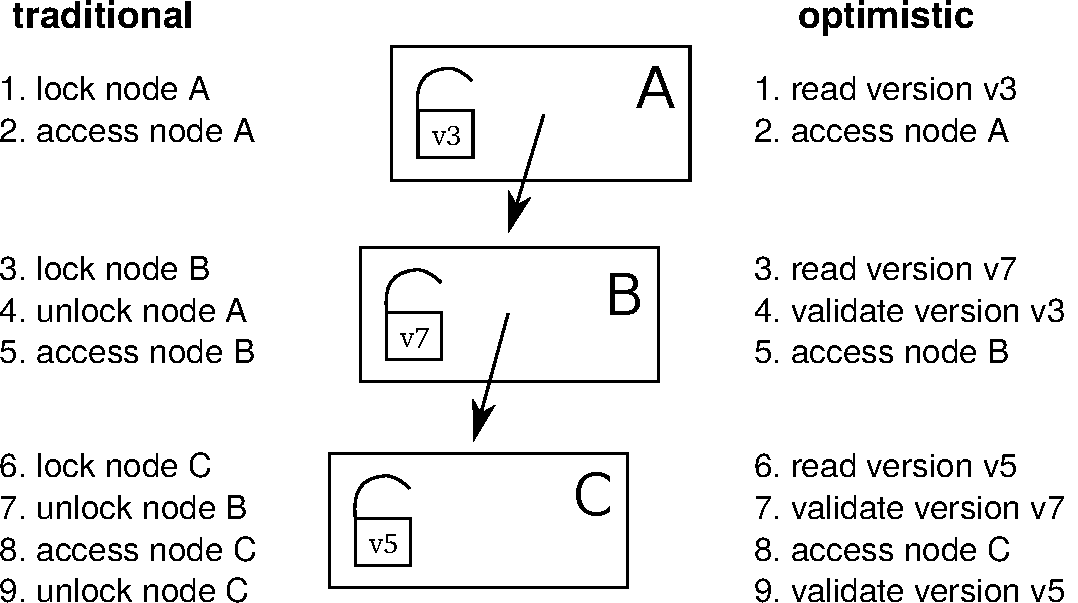
\includegraphics[width=0.65\linewidth]{olcall.pdf}
  \vspace{0.2cm}
  \caption{Comparison of a lookup operation in a 3-level tree using traditional lock coupling (left-hand side) vs.~optimistic lock coupling (right-hand side).}
  \label{fig:olc}
\end{figure}

The traditional and most common lock-based synchronization protocol for B-trees is lock coupling, which interleaves lock acquisitions while holding at most two locks at a time.
If, as we observed earlier, optimistic locks have similar semantics as traditional locks, it is natural to ask whether lock coupling can be combined with optimistic locks.
And indeed the answer is yes: One can almost mechanically translate traditional lock coupling code to optimistic lock coupling code.
This is illustrated in Figure~\ref{fig:olc}, which compares the traversal in a tree of height 3 using traditional and optimistic locks.
As the figure shows, the main difference is that locking is translated to reading the version and that unlocking becomes validation of the previously read version.
This simple change provides efficient lock-free tree traversal without the need to design a complex synchronization protocol.

It is important to emphasize the conceptual simplicity of OLC in comparison to data structures that use custom protocols like the Bw-tree~\cite{DBLP:conf/icde/LevandoskiLS13a}.
To implement lock-free access, the Bw-tree requires an indirection table, delta nodes, complex splitting and merging logic, retry logic, etc.
OLC, on the other hand, can directly be applied to B-trees mostly by adding the appropriate optimistic locking code and without modifying the node layout itself.
Therefore, OpenBw-Tree, an open source implementation of the Bw-tree, requires an order of magnitude more code than a B-tree based on OLC\footnote{Both implementations are available on GitHub: \url{https://github.com/wangziqi2016/index-microbench}}.
Given how difficult it is to develop, validate, and debug lock-free code, simplicity is obviously a major advantage.

\subsection{Correctness Aspects}

\begin{figure}
  % \centering
  %[basicstyle=\normalsize\ttfamily,showstringspaces=false,columns=fullflexible,breaklines=false,breakatwhitespace=true,numbers=none,numberstyle=\small,style=C,keepspaces=true]
\begin{lstlisting}[basicstyle=\ttfamily,language=C++,numbers=left,numberstyle=\small]
std::atomic<BTreeNode*> root;

// search for key in B+tree, returns payload in resultOut
bool lookup(Key key, Value& resultOut) {
   BTreeNode* node = root.load();
   uint64_t nodeVersion = node->readLockOrRestart();
   if (node != root.load()) // make sure the root is still the root
      restart();

   BTreeInner<Key>* parent = nullptr;
   uint64_t parentVersion = 0;

   while (node->isInner()) {
      auto inner = (BTreeInner*)node;

      // unlock parent and make current node the parent
      if (parent)
         parent->readUnlockOrRestart(parentVersion);
      parent = inner;
      parentVersion = nodeVersion;

      // search for next node
      node = inner->findChild(key);
      // validate 'inner' to ensure that 'node' pointer is valid
      inner->checkOrRestart(nodeVersion);
      // now it safe to dereference 'node' pointer (read its version)
      nodeVersion = node->readLockOrRestart();
   }

   // search in leaf and retrieve payload
   auto leaf = (BTreeLeaf*)node;
   bool success = leaf->findValue(key, resultOut);

   // unlock everything
   if (parent)
      parent->readUnlockOrRestart(parentVersion);
   node->readUnlockOrRestart(nodeVersion);

   return success;
}
\end{lstlisting}
  \vspace{0.2cm}
  \caption{B-tree lookup code using OLC. For simplicity, the restart logic is not shown.}
  \label{fig:lookup}
\end{figure}

So far, we have introduced the high-level ideas behind OLC and have stressed its similarity to traditional lock coupling.
Let us now discuss some cases where the close similarity between lock coupling and OLC breaks down.
To make this more concrete, we show the B-tree lookup code in Figure~\ref{fig:lookup}.
In the code, \texttt{readLockOrRestart} reads the lock version and \texttt{readUnlockOrRestart} validates that the read was correct.

One issue with OLC is that any pointer speculatively read from a node may point to invalid memory (if that node is modified concurrently).
Dereferencing such a pointer (e.g., to read its optimistic lock), may cause a segmentation fault or undefined behavior.
In the code shown in Figure~\ref{fig:lookup}, this problem is prevented by the extra check in line 25, which ensures that the read from the node containing the pointer was correct.
Without this additional validation, the code would in line 27 dereference the pointer speculatively read in line 23.
Note that the implementation of \texttt{checkOrRestart} is actually identical to \texttt{readUnlockOrRestart}.
We chose to give it a different name to highlight the fact that this extra check would not be necessary with read/write locks.

Another potential issue with optimistic locks is code that does not terminate.
Code that speculatively accesses a node, like an intra-node binary search, should be written in a way such that it always terminates---even in the presence of concurrent writes.
Otherwise, the validation code that detects the concurrent write will never run.
The binary search of a B-tree, for example, needs to be written in such a way that each comparison makes progress.
For some data structures that do not require loops in the traversal code (like ART) termination is trivially true.

\subsection{Implementation Details}

% implementation, efficiency
To implement an optimistic lock, one can combine the lock and the version counter into a single 64-bit\footnote{Even after subtracting one bit for the lock status, a back-of-the-envelope calculation can show that 63 bits are large enough to never overflow in practice.} word~\cite{artsync}.
A typical read operation will therefore merely consist of reading this version counter atomically.
In C++11 this can be implemented using the \texttt{std::atomic} type.

On x86, atomic reads are cheap because of x86's strong memory order guarantees.
No memory fences are required for sequentially-consistent loads, which are translated (by both GCC and clang) into standard \texttt{MOV} instructions.
Hence, the only effect of \texttt{std::atomic} for loads is preventing instruction re-ordering.
This makes version access and validation cheap.
Acquiring and releasing an optimistic lock in exclusive mode has comparable cost to a traditional lock:
A fairly expensive sequentially-consistent store is needed for acquiring a lock, while a standard \texttt{MOV} suffices for releasing it.
A simple sinlock-based implementation of optimistic locks can be found in the appendix of an earlier paper~\cite{artsync}.

OLC code must be able to handle restarts since validation or lock upgrade can fail due to concurrent writers.
Restarts can easily be implemented by wrapping the data structure operation in a loop (for simplicity not shown in Figure~\ref{fig:lookup}).
Such a loop also enables limiting the number of optimistic retry operations and falling back to pessimistic locking in cases of very heavy contention.
The ability to fall back to traditional locking is a major advantage of OLC in terms of robustness over lock-free approaches, which do not have this option.

In addition to the optimistic shared mode and the exclusive mode, optimistic locks also support a ``shared pessimistic'' mode, which physically acquires the lock in shared mode (allowing multiple concurrent readers but no writers).
This mode is useful for table (or range) scans that touch many tuples on a leaf page (which would otherwise easily abort).
Finally, let us mention that large range scans and table scans, should be broken up into several per-node traversals as is done in the LeanStore~\cite{leanstore} system.

Like all lock-free data structures, but unlike traditional locking and Hardware Transactional Memory~\cite{DBLP:conf/hpca/KarnagelDRLLSL14,DBLP:journals/pvldb/MakreshanskiLS15,htmtkde}, OLC requires care when deleting (and reusing) nodes.
The reason is that a deleting thread can never be sure that a node can be reclaimed because other threads might still be optimistically reading from that node.
Therefore, standard solutions like epoch-based reclamation~\cite{DBLP:conf/sosp/TuZKLM13}, hazard pointers~\cite{DBLP:journals/tpds/Michael04}, or optimized hazard pointers~\cite{DBLP:conf/spaa/BalmauGHZ16} need to be used.
These memory reclamation techniques are, however, largely orthogonal to the synchronization protocol itself.

%-lock-free is not a strong guarantee

\newpage
\section{Evaluation}\label{sec:evaluation}

Let us now experimentally evaluate the overhead and scalability of OLC.
For the experiments, we use an in-memory B+tree implemented in C++11 using templates, which is configured to use nodes of 4096 bytes, random 8 byte keys, and 8 byte payloads.
Based on this B-tree, we compare the following synchronization approaches:
\begin{itemize}
\item an OLC implementation\footnote{An almost identical OLC implementation is available on github: \url{https://github.com/wangziqi2016/index-microbench/tree/master/BTreeOLC}}
\item a variant based on traditional lock coupling and read/write locks
\item the unsynchronized B-tree, which obviously is only correct for read-only workloads but allows measuring the overhead of synchronization
\end{itemize}
Note that earlier work has compared the OLC implementation with a Bw-tree implementation~\cite{buzzword} and other state-of-the-art in-memory index structures.

We use a Haswell EP system with an Intel Xeon E5-2687W v3 CPU, which has 10 cores (20 ``Hyper-Threads'') and 25~MB of L3 cache.
The system is running Ubuntu 18.10 and we use GCC 8.2.0 to compile our code.
The CPU counters are obtained using the Linux perf API\footnote{We use the following convenience wrapper: \url{https://github.com/viktorleis/perfevent}}.

\begin{table}
  \caption{Performance and CPU counters for lookup and insert operations in a B-tree with 100M keys. We perform 100M operations and normalize the CPU counters by that number.}
  \label{tab:overhead}
  \centering
  \begin{tabular}{lrrrrrrr}\toprule
                    &         &        &        & instruc-  & L1     & L3     & branch \\
                    & threads & M op/s & cycles & tions & misses & misses & misses \\\midrule
lookup (no sync.)   & 1       & 1.72   & 2028   & 283     & 39.1   & 14.9   & 16.1   \\
lookup (OLC)        & 1       & 1.65   & 2107   & 370     & 43.9   & 15.1   & 16.7   \\
lookup (lock coup.) & 1       & 1.72   & 2078   & 365     & 42.3   & 16.9   & 15.7   \\\midrule
insert (no sync.)   & 1       & 1.51   & 2286   & 530     & 59.8   & 31.1   & 17.3   \\
insert (OLC)        & 1       & 1.50   & 2303   & 629     & 61.2   & 31.1   & 16.5   \\
insert (lock coup.) & 1       & 1.41   & 2473   & 644     & 61.0   & 31.0   & 17.2   \\\midrule
lookup (no sync.)   & 10      & 15.48  & 2058   & 283     & 38.6   & 15.5   & 16.0   \\
lookup (OLC)        & 10      & 14.60  & 2187   & 370     & 43.8   & 15.8   & 16.8   \\
lookup (lock coup.) & 10      & 5.71   & 5591   & 379     & 54.2   & 17.0   & 14.8   \\\midrule
insert (no sync.)   & 10      & -      & -      & -       & -      & -      & -      \\
insert (OLC)        & 10      & 10.46  & 2940   & 656     & 62.0   & 32.5   & 16.8   \\
insert (lock coup.) & 10      & 7.55   & 4161   & 667     & 75.0   & 28.6   & 16.2   \\
    \bottomrule
\end{tabular}
\end{table}

Table~\ref{tab:overhead} compares the performance and CPU counters for lookup and insert operations in a B-tree with 100M keys.
With {\em single-threaded} execution, we observe that all three approaches have very similar performance.
Adding traditional or optimistic locks to unsynchronized B-tree code results in up to 30\% of additional instructions without affecting single-threaded performance much.

\begin{figure}
  \centering
  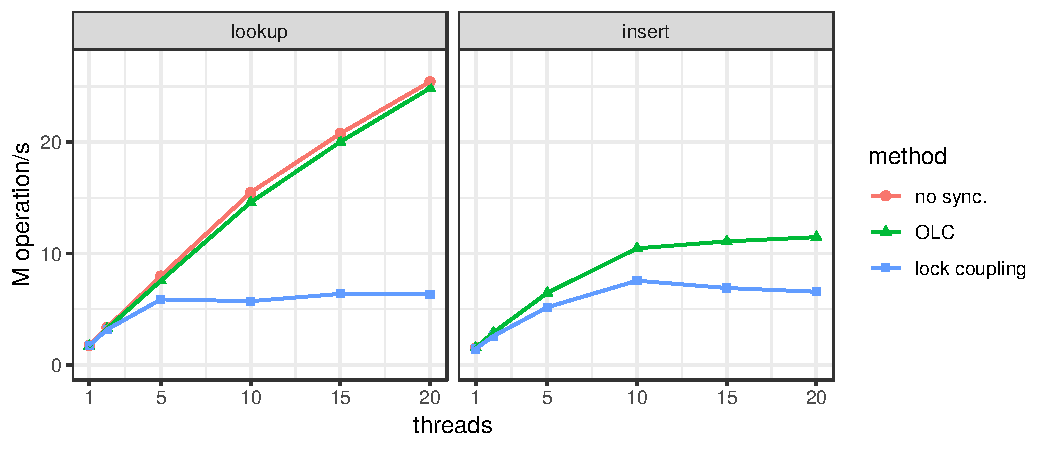
\includegraphics[width=\linewidth]{scale.pdf}
  \vspace{0.2cm}
  \caption{Scalability on 10-core system for B-tree operations (100M values).}
  \label{fig:scale}
\end{figure}

As Figure~\ref{fig:scale} shows, the results change dramatically once we use multiple threads.
For lookup, the scalability of OLC is near-linear up to 20 threads, even though the system has only 10 ``real cores''.
The OLC scalability for insert is also respectable (though not quite as linear because multi-threaded insertion approaches the memory bandwidth of our processor).
The figure also shows that the results of traditional lock coupling with read/write locks are significantly worse than OLC.
With 20 threads, lookup with OLC is 3.9$\times$ faster than traditional lock coupling.

\section{Summary}\label{sec:conc}

Optimistic Lock Coupling (OLC) is an effective synchronization method that combines the simplicity of traditional lock coupling with the superior scalability of lock-free approaches.
OLC is widely applicable and has already been successfully used to synchronize several data structures, including B-trees, binary search trees, and different trie variants.
These features make it highly attractive for modern database systems as well as performance-critical systems software in general.

\begin{thebibliography}{10}

\bibitem{DBLP:conf/spaa/BalmauGHZ16}
O.~Balmau, R.~Guerraoui, M.~Herlihy, and I.~Zablotchi.
\newblock Fast and robust memory reclamation for concurrent data structures.
\newblock In {\em SPAA}, 2016.

\bibitem{DBLP:journals/acta/BayerS77}
R.~Bayer and M.~Schkolnick.
\newblock Concurrency of operations on {B}-trees.
\newblock {\em Acta Informatica}, 9, 1977.

\bibitem{hot}
R.~Binna, E.~Zangerle, M.~Pichl, G.~Specht, and V.~Leis.
\newblock {HOT}: A height optimized trie index for main-memory database
  systems.
\newblock In {\em SIGMOD}, 2018.

\bibitem{DBLP:conf/ppopp/BronsonCCO10}
N.~G. Bronson, J.~Casper, H.~Chafi, and K.~Olukotun.
\newblock A practical concurrent binary search tree.
\newblock In {\em PPOPP}, 2010.

\bibitem{DBLP:conf/vldb/ChaHKK01}
S.~K. Cha, S.~Hwang, K.~Kim, and K.~Kwon.
\newblock Cache-conscious concurrency control of main-memory indexes on
  shared-memory multiprocessor systems.
\newblock In {\em VLDB}, 2001.

\bibitem{intel}
I.~Cutress.
\newblock {Intel} goes for 48-cores: {Cascade-AP} with multi-chip package
  coming soon.
\newblock
  \url{https://www.anandtech.com/show/13535/intel-goes-for-48cores-cascade-ap},
  2018 (accessed January, 2019).

\bibitem{DBLP:conf/cidr/FaleiroA17}
J.~M. Faleiro and D.~J. Abadi.
\newblock Latch-free synchronization in database systems: Silver bullet or
  fool's gold?
\newblock In {\em CIDR}, 2017.

\bibitem{DBLP:journals/ftdb/Graefe11}
G.~Graefe.
\newblock Modern {B}-tree techniques.
\newblock {\em Foundations and Trends in Databases}, 3(4), 2011.

\bibitem{DBLP:conf/hpca/KarnagelDRLLSL14}
T.~Karnagel, R.~Dementiev, R.~Rajwar, K.~Lai, T.~Legler, B.~Schlegel, and
  W.~Lehner.
\newblock Improving in-memory database index performance with
  {Intel}\({}^{\mbox{{\textregistered}}}\) transactional synchronization
  extensions.
\newblock In {\em HPCA}, 2014.

\bibitem{DBLP:journals/tods/LehmanY81}
P.~L. Lehman and S.~B. Yao.
\newblock Efficient locking for concurrent operations on {B}-trees.
\newblock {\em {ACM} Trans. Database Syst.}, 6(4), 1981.

\bibitem{leanstore}
V.~Leis, M.~Haubenschild, A.~Kemper, and T.~Neumann.
\newblock Leanstore: In-memory data management beyond main memory.
\newblock In {\em ICDE}, 2018.

\bibitem{art}
V.~Leis, A.~Kemper, and T.~Neumann.
\newblock The adaptive radix tree: {ARTful} indexing for main-memory databases.
\newblock In {\em ICDE}, 2013.

\bibitem{htmtkde}
V.~Leis, A.~Kemper, and T.~Neumann.
\newblock Scaling {HTM}-supported database transactions to many cores.
\newblock {\em {IEEE} Trans. Knowl. Data Eng.}, 28(2), 2016.

\bibitem{artsync}
V.~Leis, F.~Scheibner, A.~Kemper, and T.~Neumann.
\newblock The {ART} of practical synchronization.
\newblock In {\em DaMoN}, 2016.

\bibitem{DBLP:conf/icde/LevandoskiLS13a}
J.~J. Levandoski, D.~B. Lomet, and S.~Sengupta.
\newblock The {Bw}-tree: A {B}-tree for new hardware platforms.
\newblock In {\em ICDE}, 2013.

\bibitem{DBLP:journals/pvldb/MakreshanskiLS15}
D.~Makreshanski, J.~J. Levandoski, and R.~Stutsman.
\newblock To lock, swap, or elide: On the interplay of hardware transactional
  memory and lock-free indexing.
\newblock {\em {PVLDB}}, 8(11), 2015.

\bibitem{DBLP:dblp_conf/eurosys/MaoKM12}
Y.~Mao, E.~Kohler, and R.~T. Morris.
\newblock Cache craftiness for fast multicore key-value storage.
\newblock In {\em EuroSys}, 2012.

\bibitem{DBLP:journals/tpds/Michael04}
M.~M. Michael.
\newblock Hazard pointers: Safe memory reclamation for lock-free objects.
\newblock {\em {IEEE} Trans. Parallel Distrib. Syst.}, 15(6), 2004.

\bibitem{DBLP:journals/jacm/ShalevS06}
O.~Shalev and N.~Shavit.
\newblock Split-ordered lists: Lock-free extensible hash tables.
\newblock {\em J. {ACM}}, 53(3), 2006.

\bibitem{amd}
A.~Shilov.
\newblock {AMD} previews {EPYC} ‘{Rome}’ processor: Up to 64 {Zen} 2 cores.
\newblock
  \url{https://www.anandtech.com/show/13561/amd-previews-epyc-rome-processor-up-to-64-zen-2-cores},
  2018 (accessed January, 2019).

\bibitem{DBLP:conf/sosp/TuZKLM13}
S.~Tu, W.~Zheng, E.~Kohler, B.~Liskov, and S.~Madden.
\newblock Speedy transactions in multicore in-memory databases.
\newblock In {\em SOSP}, 2013.

\bibitem{buzzword}
Z.~Wang, A.~Pavlo, H.~Lim, V.~Leis, H.~Zhang, M.~Kaminsky, and D.~Andersen.
\newblock Building a {Bw}-tree takes more than just buzz words.
\newblock In {\em SIGMOD}, 2018.

\end{thebibliography}


%\bibliographystyle{abbrv}
%\bibliography{main}

\end{document}

%\end{article}
%
%
%
%\begin{article}
%{On Benchmarking for Crowdsourcing and Future of Work Platforms}
%{Ria Mae Borromeo, Lei Chen, Abhishek Dubey, Sudeepa Roy, Saravanan Thirumuruganathan}
%\graphicspath{{submissions/lei/}}
%\pdfminorversion=5
\documentclass[11pt]{article}
\usepackage{deauthor,times,graphicx,caption,microtype}
\usepackage{hyperref}
\usepackage{listings}
\usepackage{booktabs}

\begin{document}

\title{Optimistic Lock Coupling: A Scalable and Efficient General-Purpose Synchronization Method}

\author{Viktor Leis, Michael Haubenschild\raisebox{0.9ex}{$\ast$}, Thomas Neumann\\ Technische Universit{\"a}t M{\"u}nchen \hspace{0.7cm} Tableau Software\raisebox{0.9ex}{$\ast$} \\ {\{leis,neumann\}{@}in.tum.de} \hspace{0.7cm} {mhaubenschild{@}tableau.com\raisebox{0.9ex}{$\ast$}}}

\maketitle

\begin{abstract}
As the number of cores on commodity processors continues to increase, scalability becomes more and more crucial for overall performance.
Scalable and efficient concurrent data structures are particularly important, as these are often the building blocks of parallel algorithms.
Unfortunately, traditional synchronization techniques based on fine-grained locking have been shown to be unscalable on modern multi-core CPUs.
Lock-free data structures, on the other hand, are extremely difficult to design and often incur significant overhead.

In this work, we make the case for Optimistic Lock Coupling as a practical alternative to both traditional locking and the lock-free approach.
We show that Optimistic Lock Coupling is highly scalable and almost as simple to implement as traditional lock coupling.
Another important advantage is that it is easily applicable to most tree-like data structures.
We therefore argue that Optimistic Lock Coupling, rather than a complex and error-prone custom synchronization protocol, should be the default choice for performance-critical data structures.
\end{abstract}

\section{Introduction}

% more and more cores
Today, Intel's commodity server processors have up to 28 cores and its upcoming microarchitecture will have up to 48 cores per socket~\cite{intel}.
Similarly, AMD currently stands at 32 cores and this number is expected to double in the next generation~\cite{amd}.
Since both platforms support simultaneous multithreading (also known as hyperthreading), affordable commodity servers (with up to two sockets) will soon routinely have between 100 and 200 hardware threads.

% data structure scalability is important
With such a high degree of hardware parallelism, efficient data processing crucially depends on how well concurrent data structures scale.
Internally, database systems use a plethora of data structures like table heaps, internal work queues, and, most importantly, index structures.
Any of these can easily become a scalability (and therefore overall performance) bottleneck on many-core CPUs.

% traditional synchronization: fine-grained locks, slow, cache invalidation
Traditionally, database systems synchronize internal data structures using fine-grained reader/writer locks\footnote{In this work, we focus on data structure synchronization rather than high-level transaction semantics and therefore use the term {\em lock} for what would typically be called {\em latch} in the database literature. We thus follow common computer science (rather than database) terminology.}.
Unfortunately, while fine-grained locking makes lock contention unlikely, it still results in bad scalability because lock acquisition and release require writing to shared memory.
Due to the way cache coherency is implemented on modern multi-core CPUs, these writes cause additional cache misses\footnote{The cache coherency protocol ensures that all copies of a cache line on other cores are invalidated before the write can proceed.} and the cache line containing the lock's internal data becomes a point of physical contention.
As a result, any frequently-accessed lock (e.g., the lock of the root node of a B-tree) severely limits scalability.

% lock-free bw-tree: no more latches, but indirections, extremely complex
Lock-free data structures like the Bw-tree~\cite{DBLP:conf/icde/LevandoskiLS13a} (a lock-free B-tree variant) or the Split-Ordered List~\cite{DBLP:journals/jacm/ShalevS06} (a lock-free hash table) do not acquire any locks and therefore generally scale much better than locking-based approaches (in particular for read-mostly workloads).
However, lock-free synchronization has other downsides:
First, it is very difficult and results in extremely complex and error-prone code (when compared to locking).
Second, because the functionality of atomic primitives provided by the hardware (e.g., atomically compare-and-swap 8 bytes) is limited, complex operations require additional indirections within the data structure.
For example, the Bw-tree requires an indirection table and the Split-Ordered List requires ``dummy nodes'', resulting in overhead due to additional cache misses.

% OLC for the win
In this paper we make the case for {\em Optimistic Lock Coupling (OLC)}, a synchronization method that combines some of the best properties of lock-based and lock-free synchronization.
OLC utilizes a special lock type that can be used in two modes:
The first mode is similar to a traditional mutex and excludes other threads by physically acquiring the underlying lock.
In the second mode, reads can proceed optimistically by validating a version counter that is embedded in the lock (similar to optimistic concurrency control).
The first mode is typically used by writers and the second mode by readers.
Besides this special lock type, OLC is based on the observation that optimistic lock validations can be interleaved/coupled---similar to the pair-wise interleaved lock acquisition of traditional lock coupling.
Hence, the name Optimistic Lock Coupling.

OLC has a number of desirable features:
\begin{itemize}
\item By reducing the number of writes to shared memory locations and thereby avoiding cache invalidations, it {\bf scales well} for most workloads.
\item In comparison to unsynchronized code, it requires few additional CPU instructions making it {\bf efficient}.
\item OLC is {\bf widely applicable} to different data structures. It has already been successfully used for synchronizing binary search trees~\cite{DBLP:conf/ppopp/BronsonCCO10}, tries~\cite{artsync}, trie/B-tree hybrids~\cite{DBLP:dblp_conf/eurosys/MaoKM12}, and B-trees~\cite{buzzword}.
\item In comparison to the lock-free paradigm, it is also {\bf easy to use} and requires few modifications to existing, single-threaded data structures.
\end{itemize}
Despite these positive features and its simplicity, OLC is not yet widely known.
The goal of this paper is therefore to popularize this simple idea and to make a case for it.
We argue that OLC deserves to be widely known.
It is a good default synchronization paradigm---more complex, data structure-specific protocols are seldom beneficial.

The rest of the paper is organized as follows.
Section~\ref{sec:related} discusses related work, tracing the history of OLC and its underlying ideas in the literature.
The core of the paper is Section~\ref{sec:olc}, which describes the ideas behind OLC and how it can be used to synchronize complex data structures.
In Section~\ref{sec:evaluation} we experimentally show that OLC has low overhead and scales well when used to synchronize an in-memory B-tree.
We summarize the paper in Section~\ref{sec:conc}.

\newpage
\section{Related Work}\label{sec:related}

Lock coupling has been proposed as a method for allowing concurrent operations on B-trees in 1977~\cite{DBLP:journals/acta/BayerS77}.
This traditional and still widely-used method, described in detail in Graefe's B-tree survey~\cite{DBLP:journals/ftdb/Graefe11}, is also called ``latch coupling'', ``hand-over-hand locking'', and ``crabbing''.
Because at most two locks are held at-a-time during tree traversal, this technique seemingly allows for a high degree of parallelism---in particular if read/write locks are used to enable inner nodes to be locked in shared mode.
However, as we show in Section~\ref{sec:evaluation}, on modern hardware lock acquisition (even in shared mode) results in suboptimal scalability.

An early alternative from 1981 is a B-tree variant called B-link tree~\cite{DBLP:journals/tods/LehmanY81}, which only holds a single lock at a time.
It is based on the observation that between the release of the parent lock and the acquisition of the child lock, the only ``dangerous'' thing that could have happened is the split of a child node (assuming one does not implement merge operations).
Thus, when a split happens, the key being searched might end up on a neighboring node to the right of the current child node.
A B-link tree traversal therefore detects this condition and, if needed, transparently proceeds to the neighboring node.
Releasing the parent lock early is highly beneficial when the child node needs to be fetched from disk.
For in-memory workloads, however, the B-link tree has the same scalability issues as lock coupling (it acquires just as many locks).

The next major advance, Optimistic Latch-Free Index Traversal (OLFIT)~\cite{DBLP:conf/vldb/ChaHKK01}, was proposed in 2001.
OLFIT introduced the idea of a combined lock/update counter, which we call {\em optimistic lock}. % , for lack of a better name,
Based on these per-node optimistic locks and the synchronization protocol of the B-link tree, OLFIT finally achieves good scalability on parallel processors.
The OLFIT protocol is fairly complex, as it requires both the non-trivial B-link protocol and optimistic locks.
Furthermore, like the B-link tree protocol, it does not support merging nodes, and is specific to B-trees (cannot easily be applied to other data structures).

In the following two decades, the growth of main-memory capacity led to much research into other data structures besides the venerable B-tree.
Particularly relevant for our discussion is Bronson et al.'s~\cite{DBLP:conf/ppopp/BronsonCCO10} concurrent binary search tree, which is based on optimistic version validation and has a sophisticated, data structure-specific synchronization protocol.
To the best of our knowledge, this 2010 paper is the first that, as part of its protocol, interleaves version validation across nodes---rather than validating each node separately like OLFIT.
In that paper, this idea is called ``hand-over-hand, optimistic validation'', while we prefer the term Optimistic Lock Coupling to highlight the close resemblance to traditional lock coupling.
Similarly, Mao et al.'s~\cite{DBLP:dblp_conf/eurosys/MaoKM12} Masstree (a concurrent hybrid trie/B-tree) is also based on the same ideas, but again uses them as part of a more complex protocol.

The Adaptive Radix Tree (ART)~\cite{art} is another recent in-memory data structure, which we proposed in 2013.
In contrast to the two data structures just mentioned, it was originally designed with single-threaded performance in mind without supporting concurrency.
To add support for concurrency, we initially started designing a custom protocol called Read-Optimized Write Exclusion (ROWEX)~\cite{artsync}, which turned out to be non-trivial and requires modifications of the underlying data structure\footnote{Note that ROWEX is already easier to apply to existing data structures than the lock-free approach. The difficulty depends on the data structure. Applying ROWEX is hard for B-trees with sorted keys and fairly easy for copy-on-write data structures like the Height Optimized Trie~\cite{hot}---with ART being somewhere in the middle.}.
However, fairly late in the project, we also realized, that OLC {\em alone} (rather than as part of a more complex protocol) is sufficient to synchronize ART.
No other changes to the data structure were necessary.
Both approaches were published and experimentally evaluated in a followup paper~\cite{artsync}, which shows that, despite its simplicity, OLC is efficient, scalable, and generally outperforms ROWEX.

Similar results were recently published regarding B-trees~\cite{buzzword}.
In this experimental study a simple OLC-based synchronization outperformed the Bw-tree~\cite{DBLP:conf/icde/LevandoskiLS13a}, a complex lock-free synchronization approach.
Another recent paper shows that for write-intensive workloads, locking often performs better than lock-free synchronization~\cite{DBLP:conf/cidr/FaleiroA17}.
These experiences indicate that OLC is a general-purpose synchronization paradigm and motivate the current paper.

%foster b-tree\cite{DBLP:journals/tods/GraefeKK12}
%Shasha theory~\cite{DBLP:journals/tods/ShashaG88}

\section{Optimistic Lock Coupling}\label{sec:olc}

% locks suck
The standard technique for inter-thread synchronization is mutual exclusion using fine-grained locks.
In a B-tree, for example, every node usually has its own associated lock, which is acquired before accessing that node.
The problem of locking on modern multi- and many-core processors is that lock acquisition and release require writing to the shared memory location that implements the lock.
This write causes exclusive ownership of the underlying cache line and invalidates copies of it on all other processor cores.
For hierarchical, tree-like data structures, the lock of the root node becomes a point of physical contention---even in read-only workloads and even when read/write locks are used.
Depending on the specific data structure, number of cores, cache coherency protocol implementation, cache topology, whether Non-Uniform Memory Access (NUMA) is used, locking can even result in multi-threaded performance that is worse than single-threaded execution.

% in b-trees this happens very much
The inherent pessimism of locking is particularly unfortunate for B-trees:
Despite the fact that logical modifications of the root node are very infrequent, every B-tree operation must lock the root node during tree traversal\footnote{To a lesser extent this obviously applies to all inner nodes, not just the root.}.
Even the vast majority of update operations (with the exception of splits and merges), only modify a single leaf node.
These observations indicate that a more optimistic approach, which does not require locking inner nodes, would be very beneficial for B-trees.

\subsection{Optimistic Locks}

% optimism to the rescue
As the name indicates, optimistic locks try to solve the scalability issues of traditional locks using an optimistic approach.
Instead of always physically acquiring locks, even for nodes that are unlikely to be modified simultaneously, after-the-fact validation is used to detect conflicts.
This is done by augmenting each lock with a version/update counter that is incremented on every modification.
Using this version counter, readers can optimistically proceed before validating that the version did not change to ensure that the read was safe.
If validation fails, the operation is restarted.

% details on opt locks
Using optimistic locks, a read-only node access (i.e., the majority of all operations in a B-tree) does not acquire the lock and does not increment the version counter.
Instead, it performs the following steps:
\begin{enumerate}
\item read lock version (restart if lock is not free)
\item access node
\item read the version again and validate that it has not changed in the meantime
\end{enumerate}
If the last step (the validation) fails, the operation has to be restarted.
Write operations, on the other hand, are more similar to traditional locking:
\begin{enumerate}
\item acquire lock (wait if necessary)
\item access/write to node
\item increment version and unlock node
\end{enumerate}
Writes can therefore protect a node from other writes.

% similar to locks
As we observed in an earlier paper~\cite{artsync}, because of similar semantics, optimistic locks can be hidden behind an API very similar to traditional read/write locks.
Both approaches have an exclusive lock mode, and acquiring a traditional lock in shared mode is analogous to optimistic version validation.
Furthermore, like with some implementations of traditional read/write locks, optimistic locks allow upgrading a shared lock to an exclusive lock.
Lock upgrades are, for example, used to avoid most B-tree update operations from having to lock inner nodes.
In our experience, the close resemblance of optimistic and traditional locks simplifies the reasoning about optimistic locks;
one can apply similar thinking as in traditional lock-based protocols.

\subsection{Lock Coupling with Optimistic Locks}

\begin{figure}
  \centering
  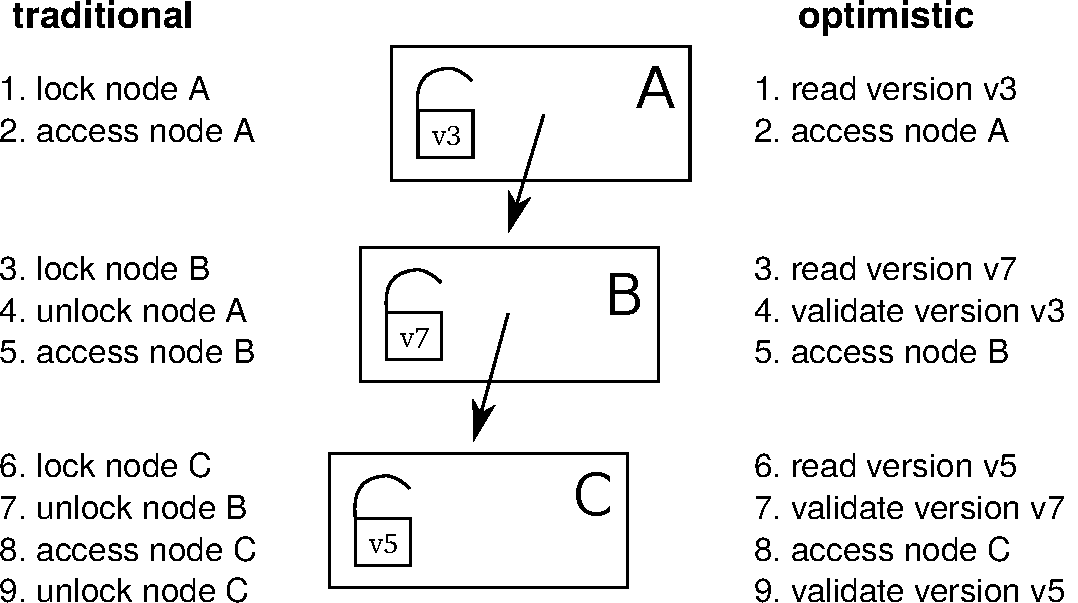
\includegraphics[width=0.65\linewidth]{olcall.pdf}
  \vspace{0.2cm}
  \caption{Comparison of a lookup operation in a 3-level tree using traditional lock coupling (left-hand side) vs.~optimistic lock coupling (right-hand side).}
  \label{fig:olc}
\end{figure}

The traditional and most common lock-based synchronization protocol for B-trees is lock coupling, which interleaves lock acquisitions while holding at most two locks at a time.
If, as we observed earlier, optimistic locks have similar semantics as traditional locks, it is natural to ask whether lock coupling can be combined with optimistic locks.
And indeed the answer is yes: One can almost mechanically translate traditional lock coupling code to optimistic lock coupling code.
This is illustrated in Figure~\ref{fig:olc}, which compares the traversal in a tree of height 3 using traditional and optimistic locks.
As the figure shows, the main difference is that locking is translated to reading the version and that unlocking becomes validation of the previously read version.
This simple change provides efficient lock-free tree traversal without the need to design a complex synchronization protocol.

It is important to emphasize the conceptual simplicity of OLC in comparison to data structures that use custom protocols like the Bw-tree~\cite{DBLP:conf/icde/LevandoskiLS13a}.
To implement lock-free access, the Bw-tree requires an indirection table, delta nodes, complex splitting and merging logic, retry logic, etc.
OLC, on the other hand, can directly be applied to B-trees mostly by adding the appropriate optimistic locking code and without modifying the node layout itself.
Therefore, OpenBw-Tree, an open source implementation of the Bw-tree, requires an order of magnitude more code than a B-tree based on OLC\footnote{Both implementations are available on GitHub: \url{https://github.com/wangziqi2016/index-microbench}}.
Given how difficult it is to develop, validate, and debug lock-free code, simplicity is obviously a major advantage.

\subsection{Correctness Aspects}

\begin{figure}
  % \centering
  %[basicstyle=\normalsize\ttfamily,showstringspaces=false,columns=fullflexible,breaklines=false,breakatwhitespace=true,numbers=none,numberstyle=\small,style=C,keepspaces=true]
\begin{lstlisting}[basicstyle=\ttfamily,language=C++,numbers=left,numberstyle=\small]
std::atomic<BTreeNode*> root;

// search for key in B+tree, returns payload in resultOut
bool lookup(Key key, Value& resultOut) {
   BTreeNode* node = root.load();
   uint64_t nodeVersion = node->readLockOrRestart();
   if (node != root.load()) // make sure the root is still the root
      restart();

   BTreeInner<Key>* parent = nullptr;
   uint64_t parentVersion = 0;

   while (node->isInner()) {
      auto inner = (BTreeInner*)node;

      // unlock parent and make current node the parent
      if (parent)
         parent->readUnlockOrRestart(parentVersion);
      parent = inner;
      parentVersion = nodeVersion;

      // search for next node
      node = inner->findChild(key);
      // validate 'inner' to ensure that 'node' pointer is valid
      inner->checkOrRestart(nodeVersion);
      // now it safe to dereference 'node' pointer (read its version)
      nodeVersion = node->readLockOrRestart();
   }

   // search in leaf and retrieve payload
   auto leaf = (BTreeLeaf*)node;
   bool success = leaf->findValue(key, resultOut);

   // unlock everything
   if (parent)
      parent->readUnlockOrRestart(parentVersion);
   node->readUnlockOrRestart(nodeVersion);

   return success;
}
\end{lstlisting}
  \vspace{0.2cm}
  \caption{B-tree lookup code using OLC. For simplicity, the restart logic is not shown.}
  \label{fig:lookup}
\end{figure}

So far, we have introduced the high-level ideas behind OLC and have stressed its similarity to traditional lock coupling.
Let us now discuss some cases where the close similarity between lock coupling and OLC breaks down.
To make this more concrete, we show the B-tree lookup code in Figure~\ref{fig:lookup}.
In the code, \texttt{readLockOrRestart} reads the lock version and \texttt{readUnlockOrRestart} validates that the read was correct.

One issue with OLC is that any pointer speculatively read from a node may point to invalid memory (if that node is modified concurrently).
Dereferencing such a pointer (e.g., to read its optimistic lock), may cause a segmentation fault or undefined behavior.
In the code shown in Figure~\ref{fig:lookup}, this problem is prevented by the extra check in line 25, which ensures that the read from the node containing the pointer was correct.
Without this additional validation, the code would in line 27 dereference the pointer speculatively read in line 23.
Note that the implementation of \texttt{checkOrRestart} is actually identical to \texttt{readUnlockOrRestart}.
We chose to give it a different name to highlight the fact that this extra check would not be necessary with read/write locks.

Another potential issue with optimistic locks is code that does not terminate.
Code that speculatively accesses a node, like an intra-node binary search, should be written in a way such that it always terminates---even in the presence of concurrent writes.
Otherwise, the validation code that detects the concurrent write will never run.
The binary search of a B-tree, for example, needs to be written in such a way that each comparison makes progress.
For some data structures that do not require loops in the traversal code (like ART) termination is trivially true.

\subsection{Implementation Details}

% implementation, efficiency
To implement an optimistic lock, one can combine the lock and the version counter into a single 64-bit\footnote{Even after subtracting one bit for the lock status, a back-of-the-envelope calculation can show that 63 bits are large enough to never overflow in practice.} word~\cite{artsync}.
A typical read operation will therefore merely consist of reading this version counter atomically.
In C++11 this can be implemented using the \texttt{std::atomic} type.

On x86, atomic reads are cheap because of x86's strong memory order guarantees.
No memory fences are required for sequentially-consistent loads, which are translated (by both GCC and clang) into standard \texttt{MOV} instructions.
Hence, the only effect of \texttt{std::atomic} for loads is preventing instruction re-ordering.
This makes version access and validation cheap.
Acquiring and releasing an optimistic lock in exclusive mode has comparable cost to a traditional lock:
A fairly expensive sequentially-consistent store is needed for acquiring a lock, while a standard \texttt{MOV} suffices for releasing it.
A simple sinlock-based implementation of optimistic locks can be found in the appendix of an earlier paper~\cite{artsync}.

OLC code must be able to handle restarts since validation or lock upgrade can fail due to concurrent writers.
Restarts can easily be implemented by wrapping the data structure operation in a loop (for simplicity not shown in Figure~\ref{fig:lookup}).
Such a loop also enables limiting the number of optimistic retry operations and falling back to pessimistic locking in cases of very heavy contention.
The ability to fall back to traditional locking is a major advantage of OLC in terms of robustness over lock-free approaches, which do not have this option.

In addition to the optimistic shared mode and the exclusive mode, optimistic locks also support a ``shared pessimistic'' mode, which physically acquires the lock in shared mode (allowing multiple concurrent readers but no writers).
This mode is useful for table (or range) scans that touch many tuples on a leaf page (which would otherwise easily abort).
Finally, let us mention that large range scans and table scans, should be broken up into several per-node traversals as is done in the LeanStore~\cite{leanstore} system.

Like all lock-free data structures, but unlike traditional locking and Hardware Transactional Memory~\cite{DBLP:conf/hpca/KarnagelDRLLSL14,DBLP:journals/pvldb/MakreshanskiLS15,htmtkde}, OLC requires care when deleting (and reusing) nodes.
The reason is that a deleting thread can never be sure that a node can be reclaimed because other threads might still be optimistically reading from that node.
Therefore, standard solutions like epoch-based reclamation~\cite{DBLP:conf/sosp/TuZKLM13}, hazard pointers~\cite{DBLP:journals/tpds/Michael04}, or optimized hazard pointers~\cite{DBLP:conf/spaa/BalmauGHZ16} need to be used.
These memory reclamation techniques are, however, largely orthogonal to the synchronization protocol itself.

%-lock-free is not a strong guarantee

\newpage
\section{Evaluation}\label{sec:evaluation}

Let us now experimentally evaluate the overhead and scalability of OLC.
For the experiments, we use an in-memory B+tree implemented in C++11 using templates, which is configured to use nodes of 4096 bytes, random 8 byte keys, and 8 byte payloads.
Based on this B-tree, we compare the following synchronization approaches:
\begin{itemize}
\item an OLC implementation\footnote{An almost identical OLC implementation is available on github: \url{https://github.com/wangziqi2016/index-microbench/tree/master/BTreeOLC}}
\item a variant based on traditional lock coupling and read/write locks
\item the unsynchronized B-tree, which obviously is only correct for read-only workloads but allows measuring the overhead of synchronization
\end{itemize}
Note that earlier work has compared the OLC implementation with a Bw-tree implementation~\cite{buzzword} and other state-of-the-art in-memory index structures.

We use a Haswell EP system with an Intel Xeon E5-2687W v3 CPU, which has 10 cores (20 ``Hyper-Threads'') and 25~MB of L3 cache.
The system is running Ubuntu 18.10 and we use GCC 8.2.0 to compile our code.
The CPU counters are obtained using the Linux perf API\footnote{We use the following convenience wrapper: \url{https://github.com/viktorleis/perfevent}}.

\begin{table}
  \caption{Performance and CPU counters for lookup and insert operations in a B-tree with 100M keys. We perform 100M operations and normalize the CPU counters by that number.}
  \label{tab:overhead}
  \centering
  \begin{tabular}{lrrrrrrr}\toprule
                    &         &        &        & instruc-  & L1     & L3     & branch \\
                    & threads & M op/s & cycles & tions & misses & misses & misses \\\midrule
lookup (no sync.)   & 1       & 1.72   & 2028   & 283     & 39.1   & 14.9   & 16.1   \\
lookup (OLC)        & 1       & 1.65   & 2107   & 370     & 43.9   & 15.1   & 16.7   \\
lookup (lock coup.) & 1       & 1.72   & 2078   & 365     & 42.3   & 16.9   & 15.7   \\\midrule
insert (no sync.)   & 1       & 1.51   & 2286   & 530     & 59.8   & 31.1   & 17.3   \\
insert (OLC)        & 1       & 1.50   & 2303   & 629     & 61.2   & 31.1   & 16.5   \\
insert (lock coup.) & 1       & 1.41   & 2473   & 644     & 61.0   & 31.0   & 17.2   \\\midrule
lookup (no sync.)   & 10      & 15.48  & 2058   & 283     & 38.6   & 15.5   & 16.0   \\
lookup (OLC)        & 10      & 14.60  & 2187   & 370     & 43.8   & 15.8   & 16.8   \\
lookup (lock coup.) & 10      & 5.71   & 5591   & 379     & 54.2   & 17.0   & 14.8   \\\midrule
insert (no sync.)   & 10      & -      & -      & -       & -      & -      & -      \\
insert (OLC)        & 10      & 10.46  & 2940   & 656     & 62.0   & 32.5   & 16.8   \\
insert (lock coup.) & 10      & 7.55   & 4161   & 667     & 75.0   & 28.6   & 16.2   \\
    \bottomrule
\end{tabular}
\end{table}

Table~\ref{tab:overhead} compares the performance and CPU counters for lookup and insert operations in a B-tree with 100M keys.
With {\em single-threaded} execution, we observe that all three approaches have very similar performance.
Adding traditional or optimistic locks to unsynchronized B-tree code results in up to 30\% of additional instructions without affecting single-threaded performance much.

\begin{figure}
  \centering
  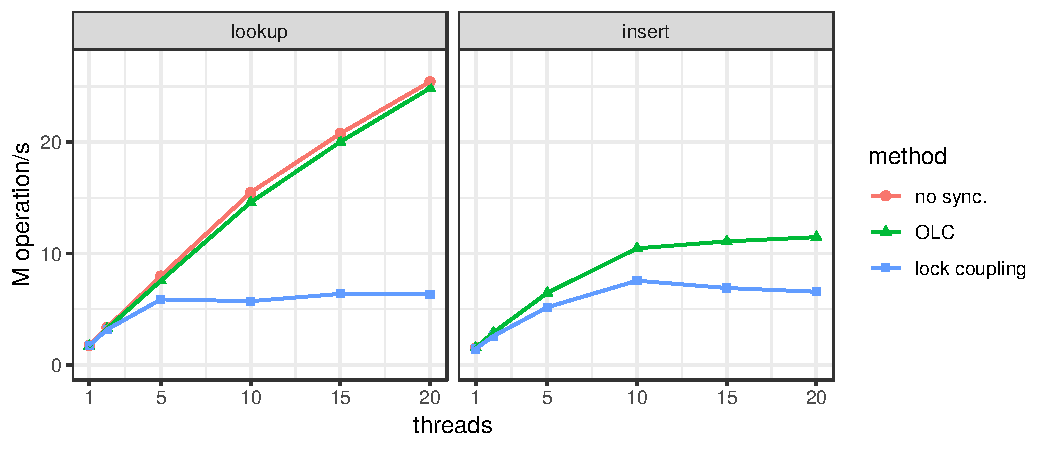
\includegraphics[width=\linewidth]{scale.pdf}
  \vspace{0.2cm}
  \caption{Scalability on 10-core system for B-tree operations (100M values).}
  \label{fig:scale}
\end{figure}

As Figure~\ref{fig:scale} shows, the results change dramatically once we use multiple threads.
For lookup, the scalability of OLC is near-linear up to 20 threads, even though the system has only 10 ``real cores''.
The OLC scalability for insert is also respectable (though not quite as linear because multi-threaded insertion approaches the memory bandwidth of our processor).
The figure also shows that the results of traditional lock coupling with read/write locks are significantly worse than OLC.
With 20 threads, lookup with OLC is 3.9$\times$ faster than traditional lock coupling.

\section{Summary}\label{sec:conc}

Optimistic Lock Coupling (OLC) is an effective synchronization method that combines the simplicity of traditional lock coupling with the superior scalability of lock-free approaches.
OLC is widely applicable and has already been successfully used to synchronize several data structures, including B-trees, binary search trees, and different trie variants.
These features make it highly attractive for modern database systems as well as performance-critical systems software in general.

\begin{thebibliography}{10}

\bibitem{DBLP:conf/spaa/BalmauGHZ16}
O.~Balmau, R.~Guerraoui, M.~Herlihy, and I.~Zablotchi.
\newblock Fast and robust memory reclamation for concurrent data structures.
\newblock In {\em SPAA}, 2016.

\bibitem{DBLP:journals/acta/BayerS77}
R.~Bayer and M.~Schkolnick.
\newblock Concurrency of operations on {B}-trees.
\newblock {\em Acta Informatica}, 9, 1977.

\bibitem{hot}
R.~Binna, E.~Zangerle, M.~Pichl, G.~Specht, and V.~Leis.
\newblock {HOT}: A height optimized trie index for main-memory database
  systems.
\newblock In {\em SIGMOD}, 2018.

\bibitem{DBLP:conf/ppopp/BronsonCCO10}
N.~G. Bronson, J.~Casper, H.~Chafi, and K.~Olukotun.
\newblock A practical concurrent binary search tree.
\newblock In {\em PPOPP}, 2010.

\bibitem{DBLP:conf/vldb/ChaHKK01}
S.~K. Cha, S.~Hwang, K.~Kim, and K.~Kwon.
\newblock Cache-conscious concurrency control of main-memory indexes on
  shared-memory multiprocessor systems.
\newblock In {\em VLDB}, 2001.

\bibitem{intel}
I.~Cutress.
\newblock {Intel} goes for 48-cores: {Cascade-AP} with multi-chip package
  coming soon.
\newblock
  \url{https://www.anandtech.com/show/13535/intel-goes-for-48cores-cascade-ap},
  2018 (accessed January, 2019).

\bibitem{DBLP:conf/cidr/FaleiroA17}
J.~M. Faleiro and D.~J. Abadi.
\newblock Latch-free synchronization in database systems: Silver bullet or
  fool's gold?
\newblock In {\em CIDR}, 2017.

\bibitem{DBLP:journals/ftdb/Graefe11}
G.~Graefe.
\newblock Modern {B}-tree techniques.
\newblock {\em Foundations and Trends in Databases}, 3(4), 2011.

\bibitem{DBLP:conf/hpca/KarnagelDRLLSL14}
T.~Karnagel, R.~Dementiev, R.~Rajwar, K.~Lai, T.~Legler, B.~Schlegel, and
  W.~Lehner.
\newblock Improving in-memory database index performance with
  {Intel}\({}^{\mbox{{\textregistered}}}\) transactional synchronization
  extensions.
\newblock In {\em HPCA}, 2014.

\bibitem{DBLP:journals/tods/LehmanY81}
P.~L. Lehman and S.~B. Yao.
\newblock Efficient locking for concurrent operations on {B}-trees.
\newblock {\em {ACM} Trans. Database Syst.}, 6(4), 1981.

\bibitem{leanstore}
V.~Leis, M.~Haubenschild, A.~Kemper, and T.~Neumann.
\newblock Leanstore: In-memory data management beyond main memory.
\newblock In {\em ICDE}, 2018.

\bibitem{art}
V.~Leis, A.~Kemper, and T.~Neumann.
\newblock The adaptive radix tree: {ARTful} indexing for main-memory databases.
\newblock In {\em ICDE}, 2013.

\bibitem{htmtkde}
V.~Leis, A.~Kemper, and T.~Neumann.
\newblock Scaling {HTM}-supported database transactions to many cores.
\newblock {\em {IEEE} Trans. Knowl. Data Eng.}, 28(2), 2016.

\bibitem{artsync}
V.~Leis, F.~Scheibner, A.~Kemper, and T.~Neumann.
\newblock The {ART} of practical synchronization.
\newblock In {\em DaMoN}, 2016.

\bibitem{DBLP:conf/icde/LevandoskiLS13a}
J.~J. Levandoski, D.~B. Lomet, and S.~Sengupta.
\newblock The {Bw}-tree: A {B}-tree for new hardware platforms.
\newblock In {\em ICDE}, 2013.

\bibitem{DBLP:journals/pvldb/MakreshanskiLS15}
D.~Makreshanski, J.~J. Levandoski, and R.~Stutsman.
\newblock To lock, swap, or elide: On the interplay of hardware transactional
  memory and lock-free indexing.
\newblock {\em {PVLDB}}, 8(11), 2015.

\bibitem{DBLP:dblp_conf/eurosys/MaoKM12}
Y.~Mao, E.~Kohler, and R.~T. Morris.
\newblock Cache craftiness for fast multicore key-value storage.
\newblock In {\em EuroSys}, 2012.

\bibitem{DBLP:journals/tpds/Michael04}
M.~M. Michael.
\newblock Hazard pointers: Safe memory reclamation for lock-free objects.
\newblock {\em {IEEE} Trans. Parallel Distrib. Syst.}, 15(6), 2004.

\bibitem{DBLP:journals/jacm/ShalevS06}
O.~Shalev and N.~Shavit.
\newblock Split-ordered lists: Lock-free extensible hash tables.
\newblock {\em J. {ACM}}, 53(3), 2006.

\bibitem{amd}
A.~Shilov.
\newblock {AMD} previews {EPYC} ‘{Rome}’ processor: Up to 64 {Zen} 2 cores.
\newblock
  \url{https://www.anandtech.com/show/13561/amd-previews-epyc-rome-processor-up-to-64-zen-2-cores},
  2018 (accessed January, 2019).

\bibitem{DBLP:conf/sosp/TuZKLM13}
S.~Tu, W.~Zheng, E.~Kohler, B.~Liskov, and S.~Madden.
\newblock Speedy transactions in multicore in-memory databases.
\newblock In {\em SOSP}, 2013.

\bibitem{buzzword}
Z.~Wang, A.~Pavlo, H.~Lim, V.~Leis, H.~Zhang, M.~Kaminsky, and D.~Andersen.
\newblock Building a {Bw}-tree takes more than just buzz words.
\newblock In {\em SIGMOD}, 2018.

\end{thebibliography}


%\bibliographystyle{abbrv}
%\bibliography{main}

\end{document}

%\end{article}
%
%
%
%\begin{article}
%{Ethical Challenges in the Future of Work}
%{Pierre Bourhis, Gianluca Demartini, Shady Elbassuoni, Emile Hoareau, H. Raghav Rao}
%\graphicspath{{submissions/gianluca/}}
%\pdfminorversion=5
\documentclass[11pt]{article}
\usepackage{deauthor,times,graphicx,caption,microtype}
\usepackage{hyperref}
\usepackage{listings}
\usepackage{booktabs}

\begin{document}

\title{Optimistic Lock Coupling: A Scalable and Efficient General-Purpose Synchronization Method}

\author{Viktor Leis, Michael Haubenschild\raisebox{0.9ex}{$\ast$}, Thomas Neumann\\ Technische Universit{\"a}t M{\"u}nchen \hspace{0.7cm} Tableau Software\raisebox{0.9ex}{$\ast$} \\ {\{leis,neumann\}{@}in.tum.de} \hspace{0.7cm} {mhaubenschild{@}tableau.com\raisebox{0.9ex}{$\ast$}}}

\maketitle

\begin{abstract}
As the number of cores on commodity processors continues to increase, scalability becomes more and more crucial for overall performance.
Scalable and efficient concurrent data structures are particularly important, as these are often the building blocks of parallel algorithms.
Unfortunately, traditional synchronization techniques based on fine-grained locking have been shown to be unscalable on modern multi-core CPUs.
Lock-free data structures, on the other hand, are extremely difficult to design and often incur significant overhead.

In this work, we make the case for Optimistic Lock Coupling as a practical alternative to both traditional locking and the lock-free approach.
We show that Optimistic Lock Coupling is highly scalable and almost as simple to implement as traditional lock coupling.
Another important advantage is that it is easily applicable to most tree-like data structures.
We therefore argue that Optimistic Lock Coupling, rather than a complex and error-prone custom synchronization protocol, should be the default choice for performance-critical data structures.
\end{abstract}

\section{Introduction}

% more and more cores
Today, Intel's commodity server processors have up to 28 cores and its upcoming microarchitecture will have up to 48 cores per socket~\cite{intel}.
Similarly, AMD currently stands at 32 cores and this number is expected to double in the next generation~\cite{amd}.
Since both platforms support simultaneous multithreading (also known as hyperthreading), affordable commodity servers (with up to two sockets) will soon routinely have between 100 and 200 hardware threads.

% data structure scalability is important
With such a high degree of hardware parallelism, efficient data processing crucially depends on how well concurrent data structures scale.
Internally, database systems use a plethora of data structures like table heaps, internal work queues, and, most importantly, index structures.
Any of these can easily become a scalability (and therefore overall performance) bottleneck on many-core CPUs.

% traditional synchronization: fine-grained locks, slow, cache invalidation
Traditionally, database systems synchronize internal data structures using fine-grained reader/writer locks\footnote{In this work, we focus on data structure synchronization rather than high-level transaction semantics and therefore use the term {\em lock} for what would typically be called {\em latch} in the database literature. We thus follow common computer science (rather than database) terminology.}.
Unfortunately, while fine-grained locking makes lock contention unlikely, it still results in bad scalability because lock acquisition and release require writing to shared memory.
Due to the way cache coherency is implemented on modern multi-core CPUs, these writes cause additional cache misses\footnote{The cache coherency protocol ensures that all copies of a cache line on other cores are invalidated before the write can proceed.} and the cache line containing the lock's internal data becomes a point of physical contention.
As a result, any frequently-accessed lock (e.g., the lock of the root node of a B-tree) severely limits scalability.

% lock-free bw-tree: no more latches, but indirections, extremely complex
Lock-free data structures like the Bw-tree~\cite{DBLP:conf/icde/LevandoskiLS13a} (a lock-free B-tree variant) or the Split-Ordered List~\cite{DBLP:journals/jacm/ShalevS06} (a lock-free hash table) do not acquire any locks and therefore generally scale much better than locking-based approaches (in particular for read-mostly workloads).
However, lock-free synchronization has other downsides:
First, it is very difficult and results in extremely complex and error-prone code (when compared to locking).
Second, because the functionality of atomic primitives provided by the hardware (e.g., atomically compare-and-swap 8 bytes) is limited, complex operations require additional indirections within the data structure.
For example, the Bw-tree requires an indirection table and the Split-Ordered List requires ``dummy nodes'', resulting in overhead due to additional cache misses.

% OLC for the win
In this paper we make the case for {\em Optimistic Lock Coupling (OLC)}, a synchronization method that combines some of the best properties of lock-based and lock-free synchronization.
OLC utilizes a special lock type that can be used in two modes:
The first mode is similar to a traditional mutex and excludes other threads by physically acquiring the underlying lock.
In the second mode, reads can proceed optimistically by validating a version counter that is embedded in the lock (similar to optimistic concurrency control).
The first mode is typically used by writers and the second mode by readers.
Besides this special lock type, OLC is based on the observation that optimistic lock validations can be interleaved/coupled---similar to the pair-wise interleaved lock acquisition of traditional lock coupling.
Hence, the name Optimistic Lock Coupling.

OLC has a number of desirable features:
\begin{itemize}
\item By reducing the number of writes to shared memory locations and thereby avoiding cache invalidations, it {\bf scales well} for most workloads.
\item In comparison to unsynchronized code, it requires few additional CPU instructions making it {\bf efficient}.
\item OLC is {\bf widely applicable} to different data structures. It has already been successfully used for synchronizing binary search trees~\cite{DBLP:conf/ppopp/BronsonCCO10}, tries~\cite{artsync}, trie/B-tree hybrids~\cite{DBLP:dblp_conf/eurosys/MaoKM12}, and B-trees~\cite{buzzword}.
\item In comparison to the lock-free paradigm, it is also {\bf easy to use} and requires few modifications to existing, single-threaded data structures.
\end{itemize}
Despite these positive features and its simplicity, OLC is not yet widely known.
The goal of this paper is therefore to popularize this simple idea and to make a case for it.
We argue that OLC deserves to be widely known.
It is a good default synchronization paradigm---more complex, data structure-specific protocols are seldom beneficial.

The rest of the paper is organized as follows.
Section~\ref{sec:related} discusses related work, tracing the history of OLC and its underlying ideas in the literature.
The core of the paper is Section~\ref{sec:olc}, which describes the ideas behind OLC and how it can be used to synchronize complex data structures.
In Section~\ref{sec:evaluation} we experimentally show that OLC has low overhead and scales well when used to synchronize an in-memory B-tree.
We summarize the paper in Section~\ref{sec:conc}.

\newpage
\section{Related Work}\label{sec:related}

Lock coupling has been proposed as a method for allowing concurrent operations on B-trees in 1977~\cite{DBLP:journals/acta/BayerS77}.
This traditional and still widely-used method, described in detail in Graefe's B-tree survey~\cite{DBLP:journals/ftdb/Graefe11}, is also called ``latch coupling'', ``hand-over-hand locking'', and ``crabbing''.
Because at most two locks are held at-a-time during tree traversal, this technique seemingly allows for a high degree of parallelism---in particular if read/write locks are used to enable inner nodes to be locked in shared mode.
However, as we show in Section~\ref{sec:evaluation}, on modern hardware lock acquisition (even in shared mode) results in suboptimal scalability.

An early alternative from 1981 is a B-tree variant called B-link tree~\cite{DBLP:journals/tods/LehmanY81}, which only holds a single lock at a time.
It is based on the observation that between the release of the parent lock and the acquisition of the child lock, the only ``dangerous'' thing that could have happened is the split of a child node (assuming one does not implement merge operations).
Thus, when a split happens, the key being searched might end up on a neighboring node to the right of the current child node.
A B-link tree traversal therefore detects this condition and, if needed, transparently proceeds to the neighboring node.
Releasing the parent lock early is highly beneficial when the child node needs to be fetched from disk.
For in-memory workloads, however, the B-link tree has the same scalability issues as lock coupling (it acquires just as many locks).

The next major advance, Optimistic Latch-Free Index Traversal (OLFIT)~\cite{DBLP:conf/vldb/ChaHKK01}, was proposed in 2001.
OLFIT introduced the idea of a combined lock/update counter, which we call {\em optimistic lock}. % , for lack of a better name,
Based on these per-node optimistic locks and the synchronization protocol of the B-link tree, OLFIT finally achieves good scalability on parallel processors.
The OLFIT protocol is fairly complex, as it requires both the non-trivial B-link protocol and optimistic locks.
Furthermore, like the B-link tree protocol, it does not support merging nodes, and is specific to B-trees (cannot easily be applied to other data structures).

In the following two decades, the growth of main-memory capacity led to much research into other data structures besides the venerable B-tree.
Particularly relevant for our discussion is Bronson et al.'s~\cite{DBLP:conf/ppopp/BronsonCCO10} concurrent binary search tree, which is based on optimistic version validation and has a sophisticated, data structure-specific synchronization protocol.
To the best of our knowledge, this 2010 paper is the first that, as part of its protocol, interleaves version validation across nodes---rather than validating each node separately like OLFIT.
In that paper, this idea is called ``hand-over-hand, optimistic validation'', while we prefer the term Optimistic Lock Coupling to highlight the close resemblance to traditional lock coupling.
Similarly, Mao et al.'s~\cite{DBLP:dblp_conf/eurosys/MaoKM12} Masstree (a concurrent hybrid trie/B-tree) is also based on the same ideas, but again uses them as part of a more complex protocol.

The Adaptive Radix Tree (ART)~\cite{art} is another recent in-memory data structure, which we proposed in 2013.
In contrast to the two data structures just mentioned, it was originally designed with single-threaded performance in mind without supporting concurrency.
To add support for concurrency, we initially started designing a custom protocol called Read-Optimized Write Exclusion (ROWEX)~\cite{artsync}, which turned out to be non-trivial and requires modifications of the underlying data structure\footnote{Note that ROWEX is already easier to apply to existing data structures than the lock-free approach. The difficulty depends on the data structure. Applying ROWEX is hard for B-trees with sorted keys and fairly easy for copy-on-write data structures like the Height Optimized Trie~\cite{hot}---with ART being somewhere in the middle.}.
However, fairly late in the project, we also realized, that OLC {\em alone} (rather than as part of a more complex protocol) is sufficient to synchronize ART.
No other changes to the data structure were necessary.
Both approaches were published and experimentally evaluated in a followup paper~\cite{artsync}, which shows that, despite its simplicity, OLC is efficient, scalable, and generally outperforms ROWEX.

Similar results were recently published regarding B-trees~\cite{buzzword}.
In this experimental study a simple OLC-based synchronization outperformed the Bw-tree~\cite{DBLP:conf/icde/LevandoskiLS13a}, a complex lock-free synchronization approach.
Another recent paper shows that for write-intensive workloads, locking often performs better than lock-free synchronization~\cite{DBLP:conf/cidr/FaleiroA17}.
These experiences indicate that OLC is a general-purpose synchronization paradigm and motivate the current paper.

%foster b-tree\cite{DBLP:journals/tods/GraefeKK12}
%Shasha theory~\cite{DBLP:journals/tods/ShashaG88}

\section{Optimistic Lock Coupling}\label{sec:olc}

% locks suck
The standard technique for inter-thread synchronization is mutual exclusion using fine-grained locks.
In a B-tree, for example, every node usually has its own associated lock, which is acquired before accessing that node.
The problem of locking on modern multi- and many-core processors is that lock acquisition and release require writing to the shared memory location that implements the lock.
This write causes exclusive ownership of the underlying cache line and invalidates copies of it on all other processor cores.
For hierarchical, tree-like data structures, the lock of the root node becomes a point of physical contention---even in read-only workloads and even when read/write locks are used.
Depending on the specific data structure, number of cores, cache coherency protocol implementation, cache topology, whether Non-Uniform Memory Access (NUMA) is used, locking can even result in multi-threaded performance that is worse than single-threaded execution.

% in b-trees this happens very much
The inherent pessimism of locking is particularly unfortunate for B-trees:
Despite the fact that logical modifications of the root node are very infrequent, every B-tree operation must lock the root node during tree traversal\footnote{To a lesser extent this obviously applies to all inner nodes, not just the root.}.
Even the vast majority of update operations (with the exception of splits and merges), only modify a single leaf node.
These observations indicate that a more optimistic approach, which does not require locking inner nodes, would be very beneficial for B-trees.

\subsection{Optimistic Locks}

% optimism to the rescue
As the name indicates, optimistic locks try to solve the scalability issues of traditional locks using an optimistic approach.
Instead of always physically acquiring locks, even for nodes that are unlikely to be modified simultaneously, after-the-fact validation is used to detect conflicts.
This is done by augmenting each lock with a version/update counter that is incremented on every modification.
Using this version counter, readers can optimistically proceed before validating that the version did not change to ensure that the read was safe.
If validation fails, the operation is restarted.

% details on opt locks
Using optimistic locks, a read-only node access (i.e., the majority of all operations in a B-tree) does not acquire the lock and does not increment the version counter.
Instead, it performs the following steps:
\begin{enumerate}
\item read lock version (restart if lock is not free)
\item access node
\item read the version again and validate that it has not changed in the meantime
\end{enumerate}
If the last step (the validation) fails, the operation has to be restarted.
Write operations, on the other hand, are more similar to traditional locking:
\begin{enumerate}
\item acquire lock (wait if necessary)
\item access/write to node
\item increment version and unlock node
\end{enumerate}
Writes can therefore protect a node from other writes.

% similar to locks
As we observed in an earlier paper~\cite{artsync}, because of similar semantics, optimistic locks can be hidden behind an API very similar to traditional read/write locks.
Both approaches have an exclusive lock mode, and acquiring a traditional lock in shared mode is analogous to optimistic version validation.
Furthermore, like with some implementations of traditional read/write locks, optimistic locks allow upgrading a shared lock to an exclusive lock.
Lock upgrades are, for example, used to avoid most B-tree update operations from having to lock inner nodes.
In our experience, the close resemblance of optimistic and traditional locks simplifies the reasoning about optimistic locks;
one can apply similar thinking as in traditional lock-based protocols.

\subsection{Lock Coupling with Optimistic Locks}

\begin{figure}
  \centering
  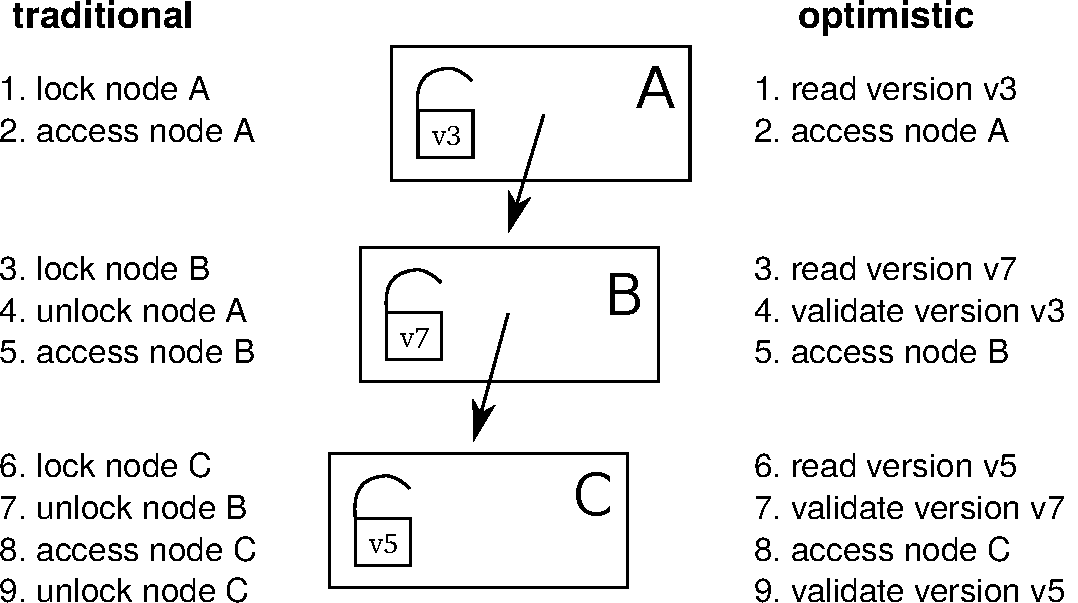
\includegraphics[width=0.65\linewidth]{olcall.pdf}
  \vspace{0.2cm}
  \caption{Comparison of a lookup operation in a 3-level tree using traditional lock coupling (left-hand side) vs.~optimistic lock coupling (right-hand side).}
  \label{fig:olc}
\end{figure}

The traditional and most common lock-based synchronization protocol for B-trees is lock coupling, which interleaves lock acquisitions while holding at most two locks at a time.
If, as we observed earlier, optimistic locks have similar semantics as traditional locks, it is natural to ask whether lock coupling can be combined with optimistic locks.
And indeed the answer is yes: One can almost mechanically translate traditional lock coupling code to optimistic lock coupling code.
This is illustrated in Figure~\ref{fig:olc}, which compares the traversal in a tree of height 3 using traditional and optimistic locks.
As the figure shows, the main difference is that locking is translated to reading the version and that unlocking becomes validation of the previously read version.
This simple change provides efficient lock-free tree traversal without the need to design a complex synchronization protocol.

It is important to emphasize the conceptual simplicity of OLC in comparison to data structures that use custom protocols like the Bw-tree~\cite{DBLP:conf/icde/LevandoskiLS13a}.
To implement lock-free access, the Bw-tree requires an indirection table, delta nodes, complex splitting and merging logic, retry logic, etc.
OLC, on the other hand, can directly be applied to B-trees mostly by adding the appropriate optimistic locking code and without modifying the node layout itself.
Therefore, OpenBw-Tree, an open source implementation of the Bw-tree, requires an order of magnitude more code than a B-tree based on OLC\footnote{Both implementations are available on GitHub: \url{https://github.com/wangziqi2016/index-microbench}}.
Given how difficult it is to develop, validate, and debug lock-free code, simplicity is obviously a major advantage.

\subsection{Correctness Aspects}

\begin{figure}
  % \centering
  %[basicstyle=\normalsize\ttfamily,showstringspaces=false,columns=fullflexible,breaklines=false,breakatwhitespace=true,numbers=none,numberstyle=\small,style=C,keepspaces=true]
\begin{lstlisting}[basicstyle=\ttfamily,language=C++,numbers=left,numberstyle=\small]
std::atomic<BTreeNode*> root;

// search for key in B+tree, returns payload in resultOut
bool lookup(Key key, Value& resultOut) {
   BTreeNode* node = root.load();
   uint64_t nodeVersion = node->readLockOrRestart();
   if (node != root.load()) // make sure the root is still the root
      restart();

   BTreeInner<Key>* parent = nullptr;
   uint64_t parentVersion = 0;

   while (node->isInner()) {
      auto inner = (BTreeInner*)node;

      // unlock parent and make current node the parent
      if (parent)
         parent->readUnlockOrRestart(parentVersion);
      parent = inner;
      parentVersion = nodeVersion;

      // search for next node
      node = inner->findChild(key);
      // validate 'inner' to ensure that 'node' pointer is valid
      inner->checkOrRestart(nodeVersion);
      // now it safe to dereference 'node' pointer (read its version)
      nodeVersion = node->readLockOrRestart();
   }

   // search in leaf and retrieve payload
   auto leaf = (BTreeLeaf*)node;
   bool success = leaf->findValue(key, resultOut);

   // unlock everything
   if (parent)
      parent->readUnlockOrRestart(parentVersion);
   node->readUnlockOrRestart(nodeVersion);

   return success;
}
\end{lstlisting}
  \vspace{0.2cm}
  \caption{B-tree lookup code using OLC. For simplicity, the restart logic is not shown.}
  \label{fig:lookup}
\end{figure}

So far, we have introduced the high-level ideas behind OLC and have stressed its similarity to traditional lock coupling.
Let us now discuss some cases where the close similarity between lock coupling and OLC breaks down.
To make this more concrete, we show the B-tree lookup code in Figure~\ref{fig:lookup}.
In the code, \texttt{readLockOrRestart} reads the lock version and \texttt{readUnlockOrRestart} validates that the read was correct.

One issue with OLC is that any pointer speculatively read from a node may point to invalid memory (if that node is modified concurrently).
Dereferencing such a pointer (e.g., to read its optimistic lock), may cause a segmentation fault or undefined behavior.
In the code shown in Figure~\ref{fig:lookup}, this problem is prevented by the extra check in line 25, which ensures that the read from the node containing the pointer was correct.
Without this additional validation, the code would in line 27 dereference the pointer speculatively read in line 23.
Note that the implementation of \texttt{checkOrRestart} is actually identical to \texttt{readUnlockOrRestart}.
We chose to give it a different name to highlight the fact that this extra check would not be necessary with read/write locks.

Another potential issue with optimistic locks is code that does not terminate.
Code that speculatively accesses a node, like an intra-node binary search, should be written in a way such that it always terminates---even in the presence of concurrent writes.
Otherwise, the validation code that detects the concurrent write will never run.
The binary search of a B-tree, for example, needs to be written in such a way that each comparison makes progress.
For some data structures that do not require loops in the traversal code (like ART) termination is trivially true.

\subsection{Implementation Details}

% implementation, efficiency
To implement an optimistic lock, one can combine the lock and the version counter into a single 64-bit\footnote{Even after subtracting one bit for the lock status, a back-of-the-envelope calculation can show that 63 bits are large enough to never overflow in practice.} word~\cite{artsync}.
A typical read operation will therefore merely consist of reading this version counter atomically.
In C++11 this can be implemented using the \texttt{std::atomic} type.

On x86, atomic reads are cheap because of x86's strong memory order guarantees.
No memory fences are required for sequentially-consistent loads, which are translated (by both GCC and clang) into standard \texttt{MOV} instructions.
Hence, the only effect of \texttt{std::atomic} for loads is preventing instruction re-ordering.
This makes version access and validation cheap.
Acquiring and releasing an optimistic lock in exclusive mode has comparable cost to a traditional lock:
A fairly expensive sequentially-consistent store is needed for acquiring a lock, while a standard \texttt{MOV} suffices for releasing it.
A simple sinlock-based implementation of optimistic locks can be found in the appendix of an earlier paper~\cite{artsync}.

OLC code must be able to handle restarts since validation or lock upgrade can fail due to concurrent writers.
Restarts can easily be implemented by wrapping the data structure operation in a loop (for simplicity not shown in Figure~\ref{fig:lookup}).
Such a loop also enables limiting the number of optimistic retry operations and falling back to pessimistic locking in cases of very heavy contention.
The ability to fall back to traditional locking is a major advantage of OLC in terms of robustness over lock-free approaches, which do not have this option.

In addition to the optimistic shared mode and the exclusive mode, optimistic locks also support a ``shared pessimistic'' mode, which physically acquires the lock in shared mode (allowing multiple concurrent readers but no writers).
This mode is useful for table (or range) scans that touch many tuples on a leaf page (which would otherwise easily abort).
Finally, let us mention that large range scans and table scans, should be broken up into several per-node traversals as is done in the LeanStore~\cite{leanstore} system.

Like all lock-free data structures, but unlike traditional locking and Hardware Transactional Memory~\cite{DBLP:conf/hpca/KarnagelDRLLSL14,DBLP:journals/pvldb/MakreshanskiLS15,htmtkde}, OLC requires care when deleting (and reusing) nodes.
The reason is that a deleting thread can never be sure that a node can be reclaimed because other threads might still be optimistically reading from that node.
Therefore, standard solutions like epoch-based reclamation~\cite{DBLP:conf/sosp/TuZKLM13}, hazard pointers~\cite{DBLP:journals/tpds/Michael04}, or optimized hazard pointers~\cite{DBLP:conf/spaa/BalmauGHZ16} need to be used.
These memory reclamation techniques are, however, largely orthogonal to the synchronization protocol itself.

%-lock-free is not a strong guarantee

\newpage
\section{Evaluation}\label{sec:evaluation}

Let us now experimentally evaluate the overhead and scalability of OLC.
For the experiments, we use an in-memory B+tree implemented in C++11 using templates, which is configured to use nodes of 4096 bytes, random 8 byte keys, and 8 byte payloads.
Based on this B-tree, we compare the following synchronization approaches:
\begin{itemize}
\item an OLC implementation\footnote{An almost identical OLC implementation is available on github: \url{https://github.com/wangziqi2016/index-microbench/tree/master/BTreeOLC}}
\item a variant based on traditional lock coupling and read/write locks
\item the unsynchronized B-tree, which obviously is only correct for read-only workloads but allows measuring the overhead of synchronization
\end{itemize}
Note that earlier work has compared the OLC implementation with a Bw-tree implementation~\cite{buzzword} and other state-of-the-art in-memory index structures.

We use a Haswell EP system with an Intel Xeon E5-2687W v3 CPU, which has 10 cores (20 ``Hyper-Threads'') and 25~MB of L3 cache.
The system is running Ubuntu 18.10 and we use GCC 8.2.0 to compile our code.
The CPU counters are obtained using the Linux perf API\footnote{We use the following convenience wrapper: \url{https://github.com/viktorleis/perfevent}}.

\begin{table}
  \caption{Performance and CPU counters for lookup and insert operations in a B-tree with 100M keys. We perform 100M operations and normalize the CPU counters by that number.}
  \label{tab:overhead}
  \centering
  \begin{tabular}{lrrrrrrr}\toprule
                    &         &        &        & instruc-  & L1     & L3     & branch \\
                    & threads & M op/s & cycles & tions & misses & misses & misses \\\midrule
lookup (no sync.)   & 1       & 1.72   & 2028   & 283     & 39.1   & 14.9   & 16.1   \\
lookup (OLC)        & 1       & 1.65   & 2107   & 370     & 43.9   & 15.1   & 16.7   \\
lookup (lock coup.) & 1       & 1.72   & 2078   & 365     & 42.3   & 16.9   & 15.7   \\\midrule
insert (no sync.)   & 1       & 1.51   & 2286   & 530     & 59.8   & 31.1   & 17.3   \\
insert (OLC)        & 1       & 1.50   & 2303   & 629     & 61.2   & 31.1   & 16.5   \\
insert (lock coup.) & 1       & 1.41   & 2473   & 644     & 61.0   & 31.0   & 17.2   \\\midrule
lookup (no sync.)   & 10      & 15.48  & 2058   & 283     & 38.6   & 15.5   & 16.0   \\
lookup (OLC)        & 10      & 14.60  & 2187   & 370     & 43.8   & 15.8   & 16.8   \\
lookup (lock coup.) & 10      & 5.71   & 5591   & 379     & 54.2   & 17.0   & 14.8   \\\midrule
insert (no sync.)   & 10      & -      & -      & -       & -      & -      & -      \\
insert (OLC)        & 10      & 10.46  & 2940   & 656     & 62.0   & 32.5   & 16.8   \\
insert (lock coup.) & 10      & 7.55   & 4161   & 667     & 75.0   & 28.6   & 16.2   \\
    \bottomrule
\end{tabular}
\end{table}

Table~\ref{tab:overhead} compares the performance and CPU counters for lookup and insert operations in a B-tree with 100M keys.
With {\em single-threaded} execution, we observe that all three approaches have very similar performance.
Adding traditional or optimistic locks to unsynchronized B-tree code results in up to 30\% of additional instructions without affecting single-threaded performance much.

\begin{figure}
  \centering
  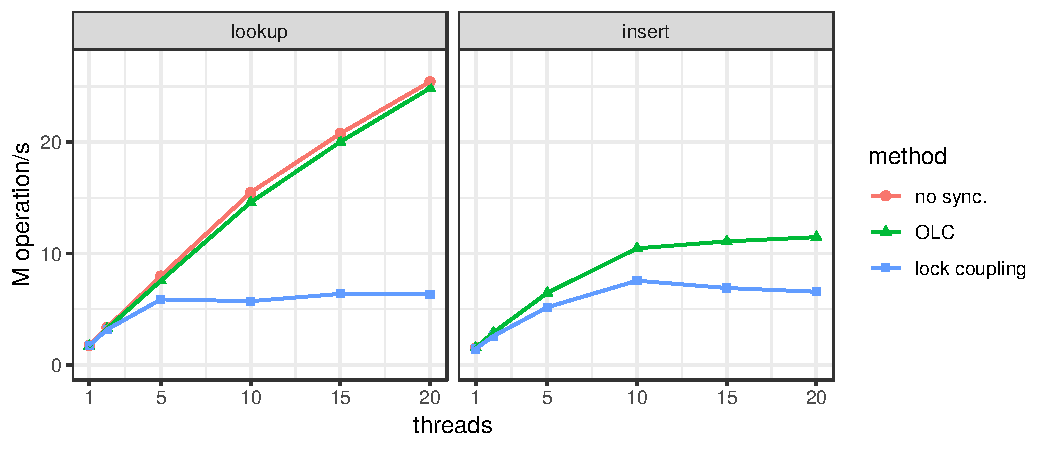
\includegraphics[width=\linewidth]{scale.pdf}
  \vspace{0.2cm}
  \caption{Scalability on 10-core system for B-tree operations (100M values).}
  \label{fig:scale}
\end{figure}

As Figure~\ref{fig:scale} shows, the results change dramatically once we use multiple threads.
For lookup, the scalability of OLC is near-linear up to 20 threads, even though the system has only 10 ``real cores''.
The OLC scalability for insert is also respectable (though not quite as linear because multi-threaded insertion approaches the memory bandwidth of our processor).
The figure also shows that the results of traditional lock coupling with read/write locks are significantly worse than OLC.
With 20 threads, lookup with OLC is 3.9$\times$ faster than traditional lock coupling.

\section{Summary}\label{sec:conc}

Optimistic Lock Coupling (OLC) is an effective synchronization method that combines the simplicity of traditional lock coupling with the superior scalability of lock-free approaches.
OLC is widely applicable and has already been successfully used to synchronize several data structures, including B-trees, binary search trees, and different trie variants.
These features make it highly attractive for modern database systems as well as performance-critical systems software in general.

\begin{thebibliography}{10}

\bibitem{DBLP:conf/spaa/BalmauGHZ16}
O.~Balmau, R.~Guerraoui, M.~Herlihy, and I.~Zablotchi.
\newblock Fast and robust memory reclamation for concurrent data structures.
\newblock In {\em SPAA}, 2016.

\bibitem{DBLP:journals/acta/BayerS77}
R.~Bayer and M.~Schkolnick.
\newblock Concurrency of operations on {B}-trees.
\newblock {\em Acta Informatica}, 9, 1977.

\bibitem{hot}
R.~Binna, E.~Zangerle, M.~Pichl, G.~Specht, and V.~Leis.
\newblock {HOT}: A height optimized trie index for main-memory database
  systems.
\newblock In {\em SIGMOD}, 2018.

\bibitem{DBLP:conf/ppopp/BronsonCCO10}
N.~G. Bronson, J.~Casper, H.~Chafi, and K.~Olukotun.
\newblock A practical concurrent binary search tree.
\newblock In {\em PPOPP}, 2010.

\bibitem{DBLP:conf/vldb/ChaHKK01}
S.~K. Cha, S.~Hwang, K.~Kim, and K.~Kwon.
\newblock Cache-conscious concurrency control of main-memory indexes on
  shared-memory multiprocessor systems.
\newblock In {\em VLDB}, 2001.

\bibitem{intel}
I.~Cutress.
\newblock {Intel} goes for 48-cores: {Cascade-AP} with multi-chip package
  coming soon.
\newblock
  \url{https://www.anandtech.com/show/13535/intel-goes-for-48cores-cascade-ap},
  2018 (accessed January, 2019).

\bibitem{DBLP:conf/cidr/FaleiroA17}
J.~M. Faleiro and D.~J. Abadi.
\newblock Latch-free synchronization in database systems: Silver bullet or
  fool's gold?
\newblock In {\em CIDR}, 2017.

\bibitem{DBLP:journals/ftdb/Graefe11}
G.~Graefe.
\newblock Modern {B}-tree techniques.
\newblock {\em Foundations and Trends in Databases}, 3(4), 2011.

\bibitem{DBLP:conf/hpca/KarnagelDRLLSL14}
T.~Karnagel, R.~Dementiev, R.~Rajwar, K.~Lai, T.~Legler, B.~Schlegel, and
  W.~Lehner.
\newblock Improving in-memory database index performance with
  {Intel}\({}^{\mbox{{\textregistered}}}\) transactional synchronization
  extensions.
\newblock In {\em HPCA}, 2014.

\bibitem{DBLP:journals/tods/LehmanY81}
P.~L. Lehman and S.~B. Yao.
\newblock Efficient locking for concurrent operations on {B}-trees.
\newblock {\em {ACM} Trans. Database Syst.}, 6(4), 1981.

\bibitem{leanstore}
V.~Leis, M.~Haubenschild, A.~Kemper, and T.~Neumann.
\newblock Leanstore: In-memory data management beyond main memory.
\newblock In {\em ICDE}, 2018.

\bibitem{art}
V.~Leis, A.~Kemper, and T.~Neumann.
\newblock The adaptive radix tree: {ARTful} indexing for main-memory databases.
\newblock In {\em ICDE}, 2013.

\bibitem{htmtkde}
V.~Leis, A.~Kemper, and T.~Neumann.
\newblock Scaling {HTM}-supported database transactions to many cores.
\newblock {\em {IEEE} Trans. Knowl. Data Eng.}, 28(2), 2016.

\bibitem{artsync}
V.~Leis, F.~Scheibner, A.~Kemper, and T.~Neumann.
\newblock The {ART} of practical synchronization.
\newblock In {\em DaMoN}, 2016.

\bibitem{DBLP:conf/icde/LevandoskiLS13a}
J.~J. Levandoski, D.~B. Lomet, and S.~Sengupta.
\newblock The {Bw}-tree: A {B}-tree for new hardware platforms.
\newblock In {\em ICDE}, 2013.

\bibitem{DBLP:journals/pvldb/MakreshanskiLS15}
D.~Makreshanski, J.~J. Levandoski, and R.~Stutsman.
\newblock To lock, swap, or elide: On the interplay of hardware transactional
  memory and lock-free indexing.
\newblock {\em {PVLDB}}, 8(11), 2015.

\bibitem{DBLP:dblp_conf/eurosys/MaoKM12}
Y.~Mao, E.~Kohler, and R.~T. Morris.
\newblock Cache craftiness for fast multicore key-value storage.
\newblock In {\em EuroSys}, 2012.

\bibitem{DBLP:journals/tpds/Michael04}
M.~M. Michael.
\newblock Hazard pointers: Safe memory reclamation for lock-free objects.
\newblock {\em {IEEE} Trans. Parallel Distrib. Syst.}, 15(6), 2004.

\bibitem{DBLP:journals/jacm/ShalevS06}
O.~Shalev and N.~Shavit.
\newblock Split-ordered lists: Lock-free extensible hash tables.
\newblock {\em J. {ACM}}, 53(3), 2006.

\bibitem{amd}
A.~Shilov.
\newblock {AMD} previews {EPYC} ‘{Rome}’ processor: Up to 64 {Zen} 2 cores.
\newblock
  \url{https://www.anandtech.com/show/13561/amd-previews-epyc-rome-processor-up-to-64-zen-2-cores},
  2018 (accessed January, 2019).

\bibitem{DBLP:conf/sosp/TuZKLM13}
S.~Tu, W.~Zheng, E.~Kohler, B.~Liskov, and S.~Madden.
\newblock Speedy transactions in multicore in-memory databases.
\newblock In {\em SOSP}, 2013.

\bibitem{buzzword}
Z.~Wang, A.~Pavlo, H.~Lim, V.~Leis, H.~Zhang, M.~Kaminsky, and D.~Andersen.
\newblock Building a {Bw}-tree takes more than just buzz words.
\newblock In {\em SIGMOD}, 2018.

\end{thebibliography}


%\bibliographystyle{abbrv}
%\bibliography{main}

\end{document}

%\end{article}
%
%\end{articlesection}

% put the news items below- there can be multiple news sections
% each with its own title
% news will usually have an author as well as a title, 
% e.g. TCDE elections
% news articles are in the same format as letters
% typically, news articles will be stored in a directory called "news"

%\begin{newssection}{News headline}

% insert news items here; news will typically have authors
% see the Sept. 2018 issue for an example

%\begin{news}{news item title}
%{author name}{author affiliation}
%\input{news/news-article.tex}
%\end{news}
%
%\newpage


%\end{newssection}



\begin{callsection}

%  This section will be empty for your version
%
%  Calls for papers section.  Use the callsection environment.
%  Each call for papers is contained in an call environment, where the single 
%  required options to \begin{call} is the name of the conference.
% typically calls are stored in a "calls" directory
%
%\begin{call}{name of conference}
%\centerline{\includegraphics[width=\textwidth, bb= 0 0 590 760]{calls/conference-name.pdf}}
%\end{call}
%\begin{call}{ICDE 2019 Conference}
%\centerline{
\includegraphics[width=\textwidth, bb= 0 0 610 790] {../Dec-2018/calls/icde19.pdf}} 
%\centerline{
\includegraphics[width=\textwidth, bb= 0 0 590 760] {calls/icde19.pdf}}
%\end{call}

\begin{call}{TCDE Membership Form}
%\centerline{\includegraphics[width=\textwidth, bb= 0 0 610 790]
\centerline{
\includegraphics[width=\textwidth, bb= 0 0 590 760] {calls/tcde.pdf}}
\end{call}

\end{callsection}

\end{bulletin}
\end{document}
